% =====================================================================
% SUPPLEMENT S4 : CE QUE LA REDUCTION RETIRE DU CORPS DE LA VERSION ENSAE (phase 4) :
% diagnostics secondaires et passages detailles dont le corps garde un resume.
% La mission envoie au supplement les diagnostics secondaires (tic T9). Chaque section reprend
% le texte retire, dans l'ordre de la reecriture des chapitres, avec sa provenance et ses
% scripts. Le texte complet d'origine reste dans chapitres/, que lit la version Institut.
% Contenu RETIRE de la version ENSAE : aucun fichier maitre ne le lit. Voir README.md.
% =====================================================================

\chapter{Compléments retirés du corps du rapport}
\label{supp:diagnostics}

\section{La fréquence seule et la forme fermée de la perte unique}
% Retire de la conclusion le 1er octobre 2026 (phase 4). Origine : chapitres/14_conclusion.tex,
% paragraphe « Le chiffre », ligne 28.
% SOURCES-SCRIPTS: 92 100

Seule, la fréquence porte le besoin de capital à $10\,377$~M\euro{}, facteur que la forme fermée de
la perte unique retrouve à moins de $1\,\%$.

% Origine : chapitres_sfe/01_contexte.tex, « Un risque de perte, de propagation et de dépendance », deplace le 2026-10-01 (phase 4). Le corps en garde un resume.
\section{Un risque de perte, de propagation et de dépendance}
% [etiquette sec:risque-cyber gardee dans le corps]

\subsection{Définition et périmètre du risque cyber}
% [etiquette subsec:definition-cyber gardee dans le corps]
% HARNAIS-HORS-SECTION: section de definitions, sans valeur chiffree issue d'un calcul du
% projet. Les seuls nombres sont des millesimes et des renvois d'articles.

Le risque cyber désigne les pertes liées à une défaillance des systèmes d'information, qu'elle
soit malveillante ou non. Cette formulation, volontairement large, recouvre l'atteinte à la
confidentialité des données, à leur intégrité et à la disponibilité des services qui en
dépendent. Elle englobe aussi bien le vol d'un fichier clients que l'arrêt d'une chaîne de
traitement, et aussi bien l'acte délibéré que l'erreur de manipulation.

Deux notions se confondent couramment et gagnent à être distinguées, car elles ne délimitent
pas le même périmètre assurable. L'\emph{incident} est tout événement, intentionnel ou non, qui
affecte la sécurité d'un système d'information : il inclut les erreurs humaines, les pannes
matérielles et les défauts de conception. La \emph{cyberattaque} en est un sous-ensemble,
caractérisé par trois conditions cumulatives, l'intention malveillante, un impact significatif
pour l'organisation et l'aboutissement effectif de l'action \citep{cesin2026}. Une tentative
neutralisée par les dispositifs de prévention n'est donc pas comptée comme une attaque, ce qui
explique qu'un même exercice puisse afficher des millions de tentatives bloquées et quelques
centaines d'attaques abouties.

Cette distinction commande le périmètre du présent travail. Le règlement DORA retient la notion
la plus large, celle de l'incident lié aux technologies de l'information et de la communication,
et non celle de la seule attaque. Une mise à jour défectueuse qui immobilise un système
d'information entre pleinement dans son champ, sans qu'aucun adversaire soit en cause. Le modèle
construit ici suit ce périmètre : il ne modélise pas une intention, il modélise une défaillance
et sa propagation.

\paragraph{Quatre familles d'incidents.} Du point de vue de leurs conséquences financières, la
diversité des modes opératoires se ramène à quatre familles.

\begin{itemize}[leftmargin=1.4em,itemsep=3pt]
\item Le \textbf{rançongiciel} chiffre les systèmes et conditionne leur restitution au versement
      d'une rançon. Son coût principal n'est en général pas la rançon mais l'interruption
      d'activité qu'il provoque et la reconstruction qu'il impose.
\item La \textbf{fuite ou le vol de données} porte atteinte à la confidentialité. Son coût se
      matérialise avec retard, par les obligations de notification, les actions de groupe et les
      sanctions du règlement général sur la protection des données.
\item Le \textbf{déni de service} rend un service indisponible sans compromettre les données. Il
      produit une perte d'exploitation nette, bornée dans le temps.
\item La \textbf{défaillance d'un prestataire ou d'un logiciel tiers} atteint simultanément tous
      ses clients. C'est la seule des quatre familles dont la perte n'est pas individualisable :
      elle produit, par construction, des sinistres corrélés.
\end{itemize}

\subsection{Des incidents individuels aux chocs de cause commune}
% [etiquette subsec:chocs-cause-commune gardee dans le corps]
% HARNAIS-HORS-SECTION: section conceptuelle, aucune valeur chiffree.

La quatrième famille change la nature du problème actuariel, et c'est elle qui justifie
l'existence de ce mémoire. Les trois premières produisent des sinistres que la mutualisation
absorbe : un portefeuille suffisamment large en lisse la charge, et la loi des grands nombres
fait son office. La quatrième produit une \emph{accumulation} que la mutualisation ne réduit
pas, puisqu'un même événement, la compromission d'un prestataire partagé, frappe simultanément
un grand nombre d'assurés qui n'ont d'autre lien entre eux que ce fournisseur.

Ce passage de l'incident individuel au choc de cause commune se joue aussi à l'intérieur d'une
seule entité, et c'est le niveau que le mémoire modélise. Les domaines de maîtrise d'une
organisation ne cèdent pas indépendamment : une gouvernance défaillante retarde la détection des
incidents ; une dépendance non maîtrisée à un prestataire ouvre une porte que les tests n'ont pas
explorée ; une détection tardive prive le partage d'informations de sa matière. La défaillance
ne reste pas dans son domaine, elle se propage.

\paragraph{Et la propagation a un sens, ce qui n'est pas un détail.} Une défaillance qui
\emph{entraîne} les autres n'appelle pas la même remédiation qu'une défaillance qui les
\emph{subit}, alors que les deux se ressemblent dans les statistiques disponibles, lesquelles
n'enregistrent qu'une co-occurrence. Distinguer ces deux situations est l'objet du mécanisme
construit au chapitre~\ref{chap:cascade}, et la difficulté de les distinguer est celle du
chapitre~\ref{ch:identifiabilite}.

\subsection{Études de cas de dépendance, de propagation et d'accumulation}
\label{subsec:cas-cyber}
% HARNAIS-HORS-SECTION: section descriptive, les seuls nombres sont des millesimes d'incidents
% publics et des ordres de grandeur de presse.

Quatre incidents publics suffisent à illustrer les trois mécanismes. Ils sont retenus non pour
leur ampleur mais parce que chacun met en défaut une hypothèse différente.

\paragraph{WannaCry, $2017$ : l'échelle de la propagation.} Un rançongiciel auto-propagable,
exploitant une faille du protocole de partage de fichiers Windows, s'est propagé en quelques
jours à des organisations de dizaines de pays, dont des hôpitaux du service de santé britannique
et des chaînes de production industrielles. Sur les onze mois qui suivent, un seul éditeur de
sécurité déclare avoir bloqué plus de $64$ millions de \emph{tentatives} en Russie et près de
$19$ millions en Ukraine comme en Inde \citep{avast2018wannacry}.

\textbf{Ces tentatives ne sont pas des sinistres, et la distinction posée à la
sous-section~\ref{subsec:definition-cyber} vaut ici pleinement.} Une tentative bloquée n'est ni
un incident ni une perte : ce que ces nombres mesurent est la \emph{persistance de l'exposition}
d'une même vulnérabilité, pas une sinistralité. Ils ne sont donc comparables à aucune grandeur du
modèle, et ils ne sont pas cités pour leur niveau. Ils établissent un seul point, qui est celui
de la sous-section~\ref{subsec:dependance-accumulation} : une vulnérabilité unique reste
sollicitée à cette échelle près d'un an après sa divulgation, si bien que l'exposition qu'elle
crée est commune à tous ceux qui la portent et n'est réduite par aucune mutualisation
(figure~\ref{fig:wannacry}).

\begin{figure}[bp]
\centering
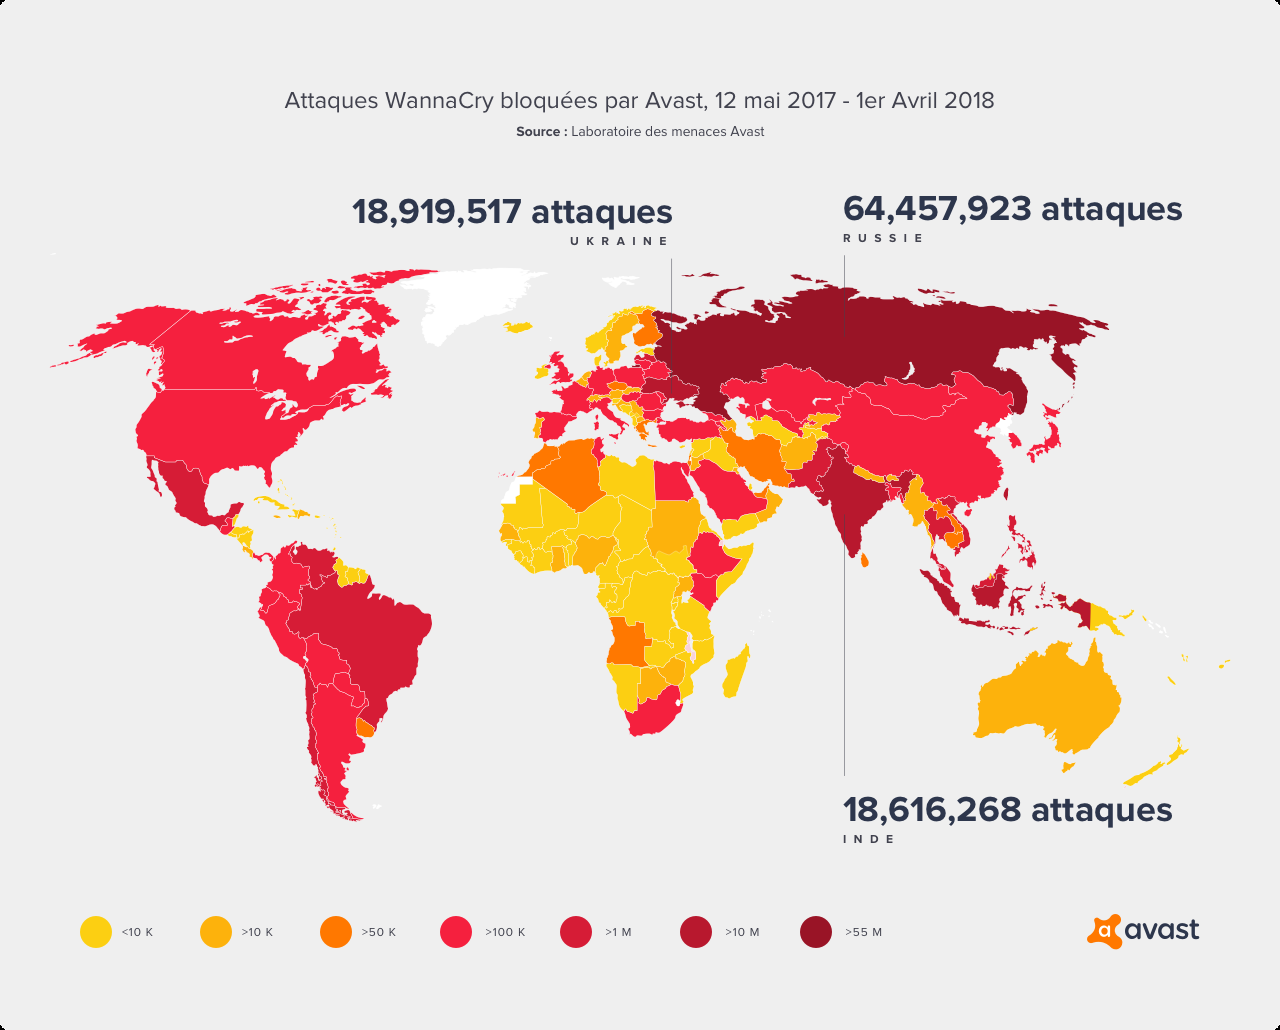
\includegraphics[width=0.85\textwidth]{figures_externes/avast_wannacry_2018_carte.png}
\caption{Tentatives d'attaque {WannaCry} bloquées par pays, $12$~mai $2017$ au $1$er~avril
$2018$. L'échelle logarithmique de la légende (de moins de $10\,000$ à plus de $55$~millions)
donne la mesure de la dispersion entre pays.
Source : laboratoire des menaces Avast \citep{avast2018wannacry}.}
\label{fig:wannacry}
\end{figure}

\paragraph{NotPetya, $2017$ : la propagation.} Un logiciel destructeur diffusé par la mise à jour
d'un logiciel comptable ukrainien s'est propagé aux réseaux de groupes internationaux et en a
paralysé l'activité pendant plusieurs semaines. L'incident naît chez un prestataire (P4), se
propage faute de cloisonnement et de gouvernance des accès (P1), et met à l'épreuve la gestion de
crise (P2). Son traitement assurantiel a en outre donné lieu à des contentieux sur l'exclusion de
guerre des contrats, ce qui rappelle qu'un sinistre cyber peut être avéré sans être couvert.

\paragraph{MOVEit, $2023$ : l'accumulation.} Une vulnérabilité d'un logiciel de transfert de
fichiers, exploitée par un groupe criminel, a permis de dérober des données chez des milliers
d'organisations, souvent atteintes à travers leurs propres prestataires. C'est un choc de cause
commune à l'état pur : une seule défaillance tierce produit de nombreux sinistres simultanés. Le
mémoire l'utilise comme expérience naturelle au chapitre~\ref{ch:identifiabilite}.

\paragraph{CrowdStrike, $2024$ : la dépendance sans adversaire.} Une mise à jour défectueuse d'un
logiciel de sécurité a bloqué des millions de postes de travail dans le transport aérien, la
banque et la santé. Aucune attaque n'est en cause : l'incident relève de la dépendance à un
prestataire (P4) et de l'absence de tests progressifs avant déploiement (P3). Il entre pleinement
dans le champ de DORA, et il montre qu'un périmètre restreint aux seules attaques manquerait une
part substantielle du risque que le règlement vise.

\medskip
\noindent Ces quatre cas ont une structure commune : un incident naît sur un domaine de contrôle
et en dégrade d'autres, dans un ordre. Aucune mesure de dépendance symétrique ne restitue cette
structure.

%======================================================================

% Origine : chapitres_sfe/01_contexte.tex, « Un risque difficile à assurer et à capitaliser », deplace le 2026-10-01 (phase 4). Le corps en garde un resume.
\section{Un risque difficile à assurer et à capitaliser}
% [etiquette sec:assurabilite-capital gardee dans le corps]

\subsection{Fréquence, sévérité et contrat d'assurance}
% [etiquette subsec:frequence-severite-contrat gardee dans le corps]
% HARNAIS-HORS-SECTION: section de cadrage actuariel, aucune valeur chiffree du projet.

La charge annuelle d'un risque se décompose classiquement en un nombre d'événements et un coût
par événement, la fréquence et la sévérité. Cette décomposition n'est pas une commodité de
présentation : elle sépare deux mécanismes que les mêmes mesures ne réduisent pas. Une
sensibilisation des collaborateurs agit sur la fréquence, une capacité de reprise agit sur la
sévérité, et un ratio agrégé qui mélange les deux ne dit pas laquelle est à l'\oe uvre. Le
mémoire applique cette discipline jusqu'au bout, en décomposant l'écart de capital entre états de
conformité plutôt qu'en l'annonçant en niveau global (chapitre~\ref{chap:resultats}).

Le contrat d'assurance introduit deux transformations qu'il faut avoir en tête avant toute
comparaison de montants. La \emph{franchise} laisse à la charge de l'assuré la première tranche
du sinistre ; la \emph{capacité} plafonne l'engagement de l'assureur. Ce que l'assureur verse
n'est donc ni la perte subie ni une fraction fixe de celle-ci, mais une perte subie transformée
par ces deux paramètres, qui varient d'un contrat à l'autre et d'un exercice à l'autre. Une
charge indemnisée et une perte brute ne se comparent ni en niveau ni en quantile.

\paragraph{Cette transformation crée une ambiguïté d'interprétation.} Sur des données agrégées,
une baisse de franchise et une aggravation réelle de la menace produisent le même signal, une
charge indemnisée qui monte. Deux mécanismes, une seule observable, et rien dans la donnée pour
les séparer. C'est, à l'échelle du marché, la situation exacte que le
chapitre~\ref{ch:identifiabilite} rencontre à l'échelle des domaines de contrôle, et le
traitement retenu y est le même : borner plutôt que poser.

\subsection{Dépendance, accumulation et risque systémique}
% [etiquette subsec:dependance-accumulation gardee dans le corps]
% HARNAIS-HORS-SECTION: section de cadrage, aucune valeur chiffree du projet.

L'assurabilité d'un risque suppose plusieurs conditions, et le cyber les met toutes en tension.
La \emph{mutualisation} suppose des sinistres suffisamment indépendants : la défaillance tierce
la met en défaut par construction. L'\emph{aléa} suppose une survenance non contrôlée par un
tiers intéressé : une attaque ciblée le contredit. La \emph{quantification} suppose un
historique suffisant, dont la sous-section suivante montre l'absence là où elle compte.
L'\emph{aléa moral} et l'\emph{anti-sélection} sont enfin renforcés par l'asymétrie
d'information entre l'assureur et l'assuré sur l'état réel du système d'information de ce
dernier.

Ce dernier point mérite d'être retenu, car c'est celui sur lequel la réglementation agit. DORA
réduit l'asymétrie : il impose un registre des accords avec les prestataires, une notification
des incidents majeurs et des tests de résilience, c'est-à-dire un ensemble d'informations
observables sur la maîtrise du risque. Une méthode qui traduit ce niveau de maîtrise en capital
utilise donc une information que le règlement rend disponible, et qui ne l'était pas avant lui.

\subsection{Rareté des données extrêmes et limite de l'historique français}
% [etiquette subsec:donnees-extremes gardee dans le corps]
% HARNAIS-HORS-SCRIPT: le niveau reglementaire 99,5 % est pose par la directive ; le recul
% de 20 % des sinistres et les millesimes 2020-2022 viennent d'analyses de sinistralite
% europeennes citees en bibliographie, que le depot ne detient pas et ne recalcule pas.

Le capital de solvabilité se mesure par un \emph{quantile} à $99{,}5\,\%$ de la charge annuelle,
c'est-à-dire par le montant qui n'est dépassé qu'une année sur deux cents. Il se joue donc
entièrement dans les sinistres les plus lourds, et non dans les sinistres courants. Or la donnée
française y est presque vide, ce que la section~\ref{sec:marche-cyber-francais} établit en
chiffres.

La conséquence est méthodologique et elle engage tout le mémoire. La méthode usuelle d'estimation
d'une queue de distribution, dite \emph{par dépassement de seuil}, ne retient que les pertes
au-dessus d'un montant élevé et ajuste une loi sur ces seules observations. Elle exige donc un
effectif suffisant au-dessus du seuil, et l'historique national n'en offre aucun : il s'arrête
avant le haut de la distribution, là précisément où se joue le quantile recherché. Une estimation
conduite sur cette base serait instable d'un exercice à l'autre et sous-estimerait le risque,
faute d'avoir observé les pertes qui le portent. C'est le motif, repris au
chapitre~\ref{chap:donnees}, de calibrer la sévérité sur une base internationale.

Cette rareté ne traduit pas une protection particulière du marché français : les analyses de
sinistres européennes relèvent un recul d'environ $20\,\%$ des sinistres cyber en $2024$ qui
laisse le niveau près d'un tiers au-dessus des exercices $2020$ à $2022$ \citep{marsh2025}, et le
marché britannique voisin est décrit comme plus développé et plus exposé aux sinistres sévères
\citep{dsit2025}.

%======================================================================

% Origine : chapitres_sfe/01_contexte.tex, « Diffusion de la couverture et fragilités techniques du marché français », deplace le 2026-10-01 (phase 4). Le corps en garde un resume.
\section{Diffusion de la couverture et fragilités techniques du marché français}
% [etiquette sec:marche-cyber-francais gardee dans le corps]

\subsection{Périmètre du portefeuille LUCY et précautions d'interprétation}
\label{subsec:lucy-perimetre}
% SOURCES-SCRIPTS: 63

L'étude LUCY de l'AMRAE, dont l'édition $2026$ porte sur l'exercice $2025$, observe le marché
français à partir de $20\,996$ polices et $1\,251$ sinistres déclarés, recueillis auprès de douze
courtiers et d'un assureur \citep{amraeLucy2026}. La série est engagée depuis $2019$, ce qui donne
sept exercices comparables et permet de distinguer un régime d'un accident d'exercice. L'auteur de
ce mémoire a co-écrit, avec son tuteur, l'analyse actuarielle de cette édition publiée par
Nexialog Consulting \citep{RapiorKaddouri2026}.

Cette source est employée sous un statut précis, celui de \emph{citation externe non
recalculable} : ses valeurs sont reprises telles qu'elle les publie, sans que le mémoire soit en
mesure de les recalculer depuis la donnée d'origine, qui ne lui appartient pas. Aucune n'entre
donc dans un calcul du modèle et aucune ne porte un montant de capital. Ce qui est vérifiable
l'est néanmoins : les valeurs sont recopiées dans un script du dépôt, qui contrôle que le rapport
des sinistres aux primes redonne bien la série des ratios publiée, que la somme des classes de
taille redonne la charge annuelle sur les sept exercices, et que chaque multiplicateur cité se
retrouve à partir des niveaux qui l'encadrent. Ces contrôles portent sur la fidélité de la
recopie, non sur la collecte ni sur le périmètre de l'étude citée, qui relèvent de celle-ci.

\begin{attention}
\textbf{Ces montants ne se comparent pas à ceux du mémoire.} La charge citée dans cette section
est une charge \emph{indemnisée}, donc nette de franchise et plafonnée par la capacité, au sens
de la sous-section~\ref{subsec:frequence-severite-contrat}. Elle vaut $83{,}2$~M\euro{} en $2025$
contre $54{,}5$ l'exercice précédent, soit une hausse de $53\,\%$. La sévérité que le présent
mémoire modélise est d'une tout autre nature : c'est la perte \emph{brute} subie par une entité
financière, avant toute assurance. Les rapprocher conduirait à lire un écart de définition comme
une contradiction.
\end{attention}

\subsection{Soft market, baisse des prix et dégradation de la sinistralité}
\label{subsec:lucy-soft-market}
% SOURCES-SCRIPTS: 63

Entre $2024$ et $2025$, le nombre d'entreprises assurées croît de $49\,\%$ quand les primes
souscrites reculent de $3\,\%$, et le ratio sinistres sur primes remonte pour le troisième
exercice, de $12\,\%$ en $2023$ à $27\,\%$ en $2025$, loin toutefois des $169\,\%$ de $2020$. Le
marché se diffuse donc par le volume et non par le budget : davantage d'entreprises sont
couvertes, pour une prime moyenne plus faible, au moment même où la sinistralité remonte
(figure~\ref{fig:lucy-ratio}).

\begin{figure}[bp]
\centering
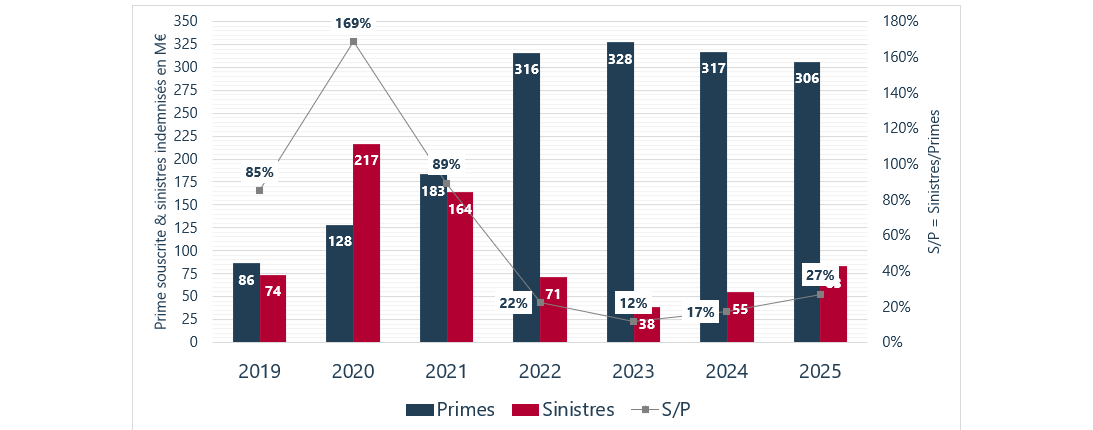
\includegraphics[width=0.85\textwidth]{figures_externes/lucy_primes_sinistres_ratio.png}
\caption{Primes souscrites, sinistres indemnisés et ratio sinistres sur primes, $2019$--$2025$.
La sinistralité remonte pour le troisième exercice consécutif alors que les primes reculent.
Source : rapport LUCY 2026, Nexialog Consulting \citep{RapiorKaddouri2026}.}
\label{fig:lucy-ratio}
\end{figure}

Cette configuration est instable par construction, et c'est ce qui donne un intérêt opérationnel
à une mesure du risque indépendante du cycle tarifaire. Le recul du taux de prime atteint
$33\,\%$ sur les grandes entreprises et $23\,\%$ sur les entreprises de taille intermédiaire :
l'assouplissement est réel, mais il ne repose sur aucune amélioration mesurée de la maîtrise du
risque.

\subsection{Un régime de sévérité en 2024, un régime de fréquence en 2025}
\label{subsec:lucy-freq-sev}
% SOURCES-SCRIPTS: 63

L'indicateur suivi par le marché est le ratio sinistres sur primes, c'est-à-dire la part de la
prime qui part en indemnisation. Il a monté deux exercices de suite, mais pour deux raisons
opposées, et seule sa décomposition le montre. La charge d'une année se met en effet sous la
forme d'un produit de deux termes, le \emph{nombre} de sinistres survenus et le \emph{sinistre
moyen}. Le tableau compare chaque terme à sa valeur de l'année précédente, sous la forme d'un
multiplicateur.

\begin{center}\small
\renewcommand{\arraystretch}{1.2}
\begin{tabular}{@{}l r r r l@{}}
\toprule
& \textbf{nombre} & \textbf{sinistre moyen} & \textbf{charge} & \textbf{régime} \\
\midrule
Marché, exercice $2024$ & $\times 0{,}73$ & $\times 1{,}96$ & $\times 1{,}43$ & sévérité \\
Marché, exercice $2025$ & $\times 2{,}79$ & $\times 0{,}55$ & $\times 1{,}53$ & fréquence \\
\midrule
\multicolumn{5}{@{}l}{\emph{Exercice $2025$, par bloc}} \\
grandes entreprises & $\times 1{,}24$ & $\times 0{,}82$ & $\times 1{,}02$ & absorbé \\
bloc intermédiaire & $\times 2{,}14$ & $\times 1{,}65$ & $\times 3{,}53$ & les deux \\
micro-entreprises & $\times 9{,}52$ & $\times 0{,}73$ & $\times 6{,}97$ & nombre seul \\
\bottomrule
\end{tabular}
\end{center}

\vspace{2pt}
\noindent En $2024$ le nombre de sinistres a baissé alors que leur coût moyen a doublé : la charge
a monté parce que les sinistres étaient plus lourds. En $2025$ c'est l'inverse, le coût moyen a
baissé de moitié alors que le nombre a presque triplé. Le ratio seul ne permet pas de distinguer
ces deux situations, qui n'appellent pourtant pas les mêmes mesures. Le bloc intermédiaire est le
seul segment où le nombre et le coût moyen augmentent en même temps, ce qui explique sa charge
multipliée par $3{,}53$.

\noindent Ces multiplicateurs portent sur le \emph{nombre} de sinistres, un total, et non sur la
\emph{fréquence}, qui le rapporte au nombre d'assurés : l'égalité charge $=$ nombre $\times$ coût
moyen n'est exacte qu'avec le nombre.

\subsection{Polarisation du marché et limites de la donnée assurantielle}
\label{subsec:lucy-polarisation}
% SOURCES-SCRIPTS: 63

La divergence entre le prix et le risque ne se répartit pas uniformément
(figure~\ref{fig:lucy-divergence}). Le segment dont la
sinistralité progresse le plus n'est pas celui dont le tarif se redresse, et les multiplicateurs
les plus spectaculaires portent sur les micro-entreprises, dont la part dans la charge totale
reste marginale. Un multiplicateur hiérarchise des dynamiques, jamais des enjeux.

\begin{figure}[bp]
\centering
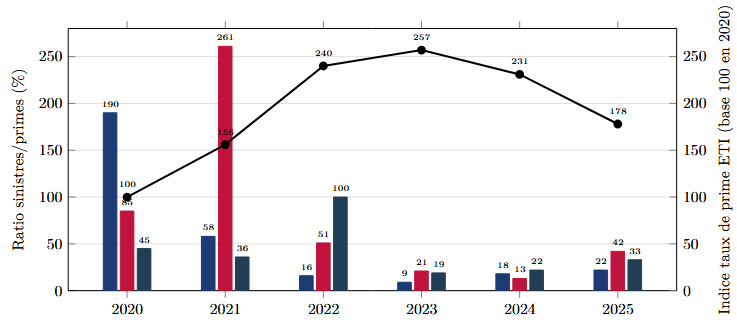
\includegraphics[width=0.85\textwidth]{figures_externes/lucy_divergence_prix_risque.png}
\caption{Divergence entre le prix et le risque par segment. Le segment dont la sinistralité
progresse le plus n'est pas celui dont le tarif se redresse.
Source : rapport LUCY 2026, Nexialog Consulting \citep{RapiorKaddouri2026}.}
\label{fig:lucy-divergence}
\end{figure}

\paragraph{La limite qui engage le mémoire est ailleurs, et elle est dans la queue.} Deux
exercices sur sept ne portent aucun sinistre de la classe de taille la plus haute ; un exercice
en porte $135$~M\euro{} et l'exercice sous revue $19$~M\euro, pour un seul sinistre dépassant
$10$~M\euro. Le maximum de la série vaut $7{,}11$ fois le montant de l'exercice sous revue, ce qui
donne la mesure de l'irrégularité (figure~\ref{fig:lucy-taille}).

% [environnement fig:lucy-taille garde dans le corps du rapport]

C'est la mesure annoncée à la sous-section~\ref{subsec:donnees-extremes}, et elle tranche le
choix de la base de calibration.

%======================================================================

% Origine : chapitres_sfe/01_contexte.tex, « Le règlement DORA, de la résilience opérationnelle à la maîtrise des dépendances », deplace le 2026-10-01 (phase 4). Le corps en garde un resume.
\section{Le règlement DORA, de la résilience opérationnelle à la maîtrise des dépendances}
% [etiquette sec:dora gardee dans le corps]
% HARNAIS-HORS-SECTION: section reglementaire. Les seuls nombres sont des millesimes, des
% numeros d'articles et des references de textes, aucun ne provient d'un calcul du projet.

\subsection{Le cadre réglementaire européen du cyber}
% [etiquette subsec:cadre-reglementaire-europeen gardee dans le corps]
% HARNAIS-HORS-SECTION: section reglementaire. Les nombres sont la date d'entree en
% application, des millesimes et des numeros officiels de textes (2022/2554, 2022/2555,
% 2022/2557, 2016/679, 2024/2847). Ce sont des donnees de droit, aucune ne vient d'un calcul.

Le cadre européen s'est construit par strates, et quatre textes en forment aujourd'hui l'ossature.
La directive sur la sécurité des réseaux et des systèmes d'information a posé des exigences
minimales de sécurité et de notification pour les opérateurs de services essentiels ; sa refonte,
dite NIS~2 \citep{NIS2Directive2022}, en a élargi le périmètre aux entités \emph{essentielles} et
\emph{importantes} et a rendu l'organe de direction responsable des mesures de gestion du risque.
Le règlement général sur la protection des données \citep{RGPD2016} fixe, en parallèle, un régime de
notification et de sanction propre aux données personnelles. La directive sur la résilience des
entités critiques \citep{REC2022} étend la même logique aux activités dont l'interruption affecte
des fonctions sociétales vitales, et vise la continuité physique autant que numérique. Le
règlement sur la cyberrésilience \citep{CRA2024}, enfin, déplace la contrainte vers l'amont : il
l'impose aux produits comportant des éléments numériques plutôt qu'à leurs utilisateurs.

Aucun de ces textes ne porte sur la continuité d'une activité financière. Les deux premiers visent
la sécurité et la confidentialité, le troisième la criticité sectorielle, le quatrième la conformité
du produit mis sur le marché. C'est ce que le règlement sur la résilience opérationnelle numérique
du secteur financier, dit DORA \citep{DORA2022}, vient combler. Entré en application le $17$ janvier $2025$, il s'adresse à une vingtaine de
catégories d'entités financières, dont les entreprises d'assurance, et il déplace l'objectif :
il ne s'agit plus seulement d'empêcher l'incident mais de garantir que l'entité \emph{résiste,
réagit et se rétablit} lorsqu'il survient. Cette bascule est celle qui rend le sujet actuariel,
car un objectif de continuité se mesure en pertes évitées et en durées d'indisponibilité, donc
en grandeurs que l'on peut chiffrer.

\paragraph{Ce que le mémoire retient de cet ensemble, et ce qu'il laisse de côté.} Seul DORA est
modélisé, et le motif est de mesure et non d'importance : il est le seul de ces textes à découper la
résilience en domaines de contrôle dont la défaillance se lit dans des données d'incidents, et le
seul dont la non-conformité s'adresse à l'entité qui porte le capital. Les autres interviennent comme
contexte. Le règlement sur la cyberrésilience, applicable à partir de décembre~$2027$, agit sur la
fréquence future des vulnérabilités logicielles, donc sur une grandeur que la calibration du
chapitre~\ref{chap:donnees} estime sur l'historique et ne projette pas. Les cadres applicables à
l'intelligence artificielle et à l'identité numérique ne sont pas traités : la cartographie de la
sous-section~\ref{subsec:france-assureurs-cesin} fait apparaître un risque lié à l'intelligence
artificielle, mais aucune source ne le rattache aujourd'hui à un domaine de contrôle de DORA, et
l'y rattacher par analogie serait poser ce que le mémoire prétend mesurer.

\subsection{Les cinq piliers de DORA}
% [etiquette subsec:cinq-piliers-dora gardee dans le corps]
% HARNAIS-HORS-SECTION: section reglementaire. Les nombres sont les etiquettes P1 a P5, les
% numeros d'articles du reglement (5 a 16, 17 a 23, 24 a 27, 26, 28 a 44, 30, 45) et les
% delais qu'il fixe. Ce sont des donnees de droit, aucune ne vient d'un calcul du projet.

Le règlement organise la résilience autour de cinq domaines, que le mémoire note P1 à P5 et
traite comme des domaines de \emph{contrôle} plutôt que comme des obligations à cocher.

\begin{itemize}[leftmargin=1.4em,itemsep=4pt]
\item \textbf{P1, gouvernance du risque lié aux technologies} (articles~$5$ à~$16$). L'organe de direction est
      explicitement responsable du dispositif, et cette responsabilité n'est pas délégable :
      stratégie de résilience, cartographie des actifs informationnels et des dépendances
      critiques, politique de sécurité documentée, et contrôle interne continu plutôt
      qu'audits ponctuels.
\item \textbf{P2, gestion, classification et notification des incidents} (articles~$17$ à~$23$). Détection,
      qualification selon des critères de matérialité, puis notification des incidents
      \emph{majeurs} selon un calendrier resserré : alerte sous quatre heures après
      classification et au plus tard vingt-quatre heures après détection, rapport
      intermédiaire sous soixante-douze heures, rapport final sous un mois.
\item \textbf{P3, tests de résilience opérationnelle numérique} (articles~$24$ à~$27$). Les procédures ne se
      documentent plus, elles s'éprouvent. Les entités identifiées comme significatives sont
      soumises à des tests de pénétration guidés par la menace (article~$26$), à mener au moins
      tous les trois ans en conditions proches du réel.
\item \textbf{P4, gestion du risque lié aux prestataires tiers} (articles~$28$ à~$44$). Recensement des contrats
      critiques dans un registre d'informations harmonisé, clauses contractuelles impératives
      de l'article~$30$,
      stratégie de sortie, et surveillance directe des prestataires tiers jugés critiques par
      les autorités européennes, jusqu'au troisième rang de la chaîne de sous-traitance.
\item \textbf{P5, partage d'informations sur les cybermenaces} (article~$45$). Échange, sur une base
      volontaire et encadrée, de renseignements entre entités financières. C'est le pilier le
      moins mobilisable dans un calibrage actuariel, et il rappelle que la résilience porte
      une dimension collective au-delà de l'entité.
\end{itemize}

\paragraph{La lecture que le mémoire en fait.} Ces cinq domaines ne sont pas indépendants, et
c'est l'hypothèse de travail de tout le document. La défaillance de l'un dégrade la capacité de
l'entité à tenir les autres, selon le mécanisme décrit à la
sous-section~\ref{subsec:chocs-cause-commune} et formalisé au chapitre~\ref{chap:cascade}. La
non-conformité ne reste pas dans son pilier.

\subsection{Prestataires TIC, concentration et propagation du risque}
% [etiquette subsec:risque-tiers-dora gardee dans le corps]
% SOURCES-SCRIPTS: 103

Le quatrième pilier est celui qui a motivé le règlement autant que les autres réunis. La chaîne
de sous-traitance informatique du secteur financier est concentrée sur un petit nombre de
fournisseurs d'infrastructure, de logiciels de gestion et de services de sécurité, si bien qu'une
défaillance chez l'un d'eux atteint simultanément de nombreuses entités sans qu'aucune n'ait
commis de faute. C'est la raison pour laquelle DORA ne se contente pas d'exiger des clauses
contractuelles : il instaure un cadre de surveillance directe des prestataires désignés comme
critiques, ce qui est une nouveauté dans l'architecture prudentielle européenne.

Cette concentration n'est pas une conjecture : la sous-section~\ref{subsec:france-assureurs-cesin}
la mesure, en montrant que l'attaque indirecte par un tiers est, parmi les vecteurs dont la part
s'élève avec la taille de l'entité, celui dont le \emph{niveau} est de loin le plus haut.

Le premier bilan des notifications la confirme du côté des victimes. En
2025, les sociétés de gestion ont adressé à l'Autorité des marchés financiers $47$
notifications initiales, dont $31$ ont été confirmées comme incidents majeurs ; $27$ d'entre
eux, soit $87\,\%$, trouvent leur origine chez un prestataire, par cyberattaque ($68\,\%$) ou
par défaillance accidentelle ($19\,\%$) \citep{amf2026incidents}. Un incident y est compté par
société déclarante, et la compromission d'un même prestataire en touche plusieurs : c'est
l'accumulation du quatrième pilier, observée sur une population entière. Cette part mesure une
origine, non une probabilité de transfert entre domaines de contrôle, et ne calibre aucun
paramètre du modèle. L'écart entre notifications et incidents confirmés annonce ce que
sera le registre : une collecte au-dessus d'un seuil de matérialité, non un recensement
exhaustif.

\paragraph{Le registre d'informations pèse plus que les autres exigences pour la modélisation.}
En imposant le recensement exhaustif des contrats TIC critiques et de leurs chaînes de
sous-traitance, le règlement produit une donnée exploitable pour modéliser le risque de
concentration technologique. Cette donnée faisait défaut à l'évaluation interne des risques
traditionnelle, qui décrivait la dépendance sans pouvoir la chiffrer. C'est le point de contact
le plus direct entre une obligation réglementaire et une entrée de modèle. La
section~\ref{ch:livrable} y revient pour dire précisément ce que ce registre donnera et ce
qu'il ne donnera pas : il porte sur les accords contractuels, donc sur la dépendance
\emph{déclarée}, et non sur l'ordre dans lequel les défaillances s'enchaînent.

\subsection{Les autorités françaises et la supervision de la résilience numérique}
\label{subsec:supervision-france}
% HARNAIS-HORS-SECTION: section institutionnelle, aucune valeur chiffree.

La supervision se répartit entre plusieurs autorités aux compétences distinctes. L'Autorité de
contrôle prudentiel et de résolution supervise les entreprises d'assurance et intègre le risque
informatique à sa démarche prudentielle ; l'Autorité des marchés financiers encadre les sociétés
de gestion ; l'Agence nationale de la sécurité des systèmes d'information porte la prévention et
la réponse aux incidents affectant les systèmes critiques ; et la Commission nationale de
l'informatique et des libertés veille au respect du régime des données personnelles. Au niveau
européen, les trois autorités de surveillance sectorielles coordonnent la désignation et la
surveillance des prestataires tiers critiques.

Cette répartition a une conséquence pour le mémoire : aucune de ces autorités ne publie de
probabilité de propagation entre domaines de contrôle. Elles publient des attentes prudentielles
et des échelles de maturité, ce qui n'est pas la même chose. C'est le motif pour lequel les
valeurs de propagation du modèle sont posées à dire d'expert puis bornées, et non présentées
comme calibrées sur une source officielle.

%======================================================================

% Origine : chapitres_sfe/01_contexte.tex, « Un risque prioritaire sans traduction prudentielle directe », deplace le 2026-10-01 (phase 4). Le corps en garde un resume.
\section{Un risque prioritaire sans traduction prudentielle directe}
% [etiquette sec:enjeu-prudentiel gardee dans le corps]

\subsection{La perception prospective selon France Assureurs et le CESIN}
% [etiquette subsec:france-assureurs-cesin gardee dans le corps]
% SOURCES-SCRIPTS: 103 63

Deux sources annuelles, de nature différente, situent le risque cyber. La cartographie
prospective de la profession classe les risques selon leur fréquence et leur gravité anticipées
\citep{franceassureurs2026} ; le baromètre mené auprès des responsables de la sécurité des
systèmes d'information recense les vecteurs et les conséquences \emph{déclarés}
\citep{cesin2026}. La première mesure une anticipation, la seconde un constat.

\paragraph{Le risque cyber sature au sommet de la cartographie.} Il occupe la première place pour
le huitième exercice consécutif, avec un score moyen de $4{,}1$ sur $5$, devant l'environnement
économique à $4{,}0$ et le dérèglement climatique à $3{,}9$. Mais son score ne monte plus : il
culmine à $4{,}48$ lors de l'édition $2022$ et redescend à $4{,}10$ en $2026$. Une préoccupation
installée au sommet d'un classement cesse d'être informative par son rang, et le renseignement
passe dans la manière dont elle se déforme (figure~\ref{fig:carto-retro}).

\begin{figure}[bp]
\centering
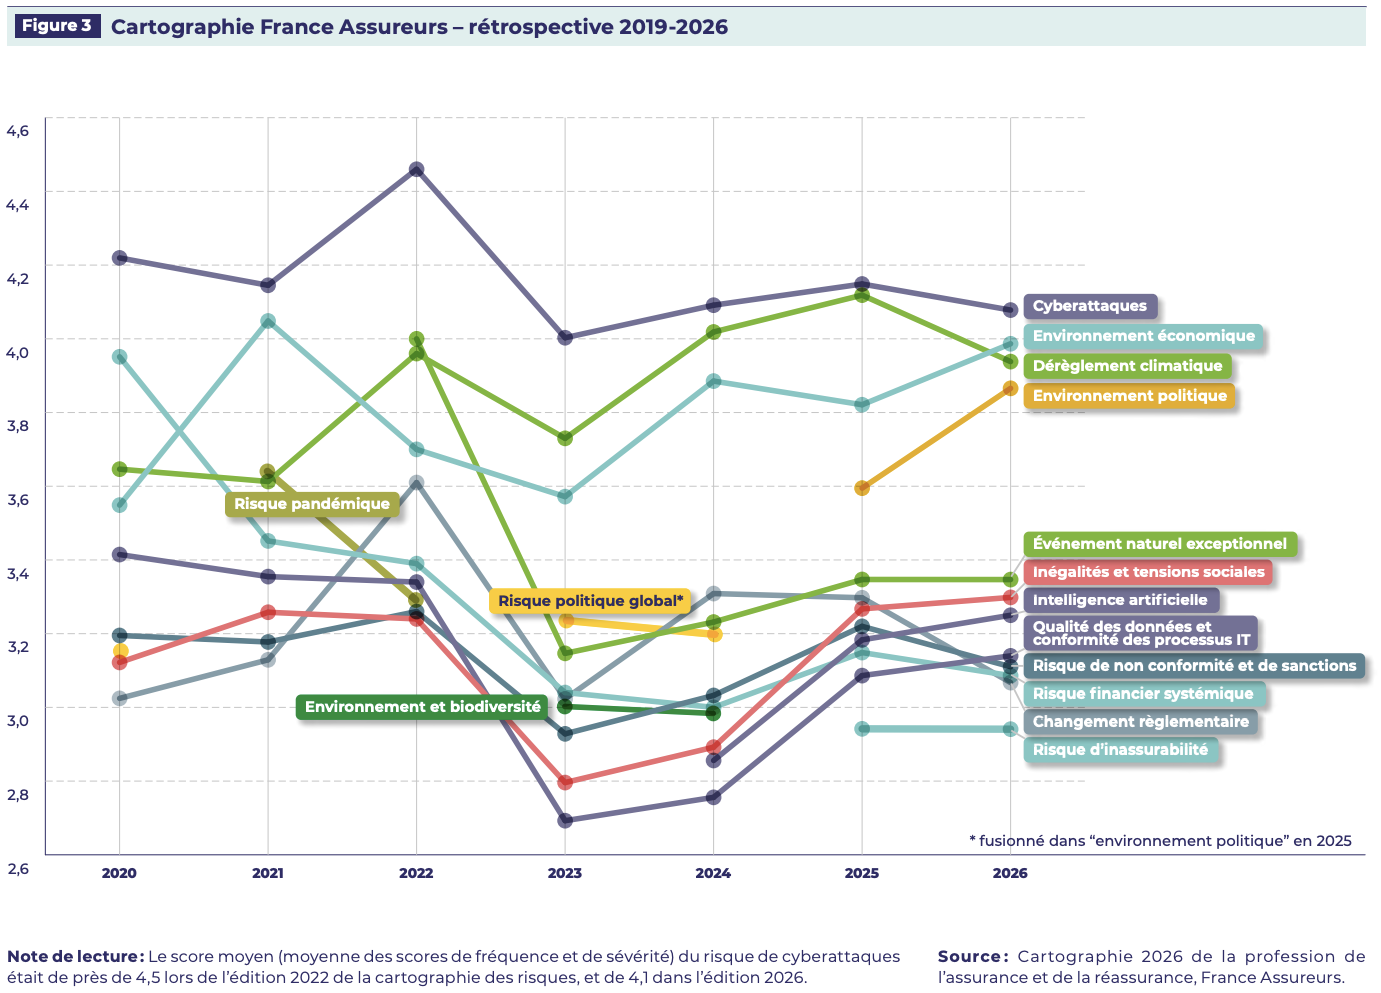
\includegraphics[width=0.92\textwidth]{figures_externes/carto_fa_2026_retrospective.png}
\caption{Trajectoire des scores de la cartographie prospective, $2020$--$2026$. Le risque de
cyberattaques reste au premier rang mais son score a cessé de monter depuis $2022$.
Source : cartographie prospective des risques, France Assureurs \citep{franceassureurs2026}.}
\label{fig:carto-retro}
\end{figure}

\paragraph{Et la déformation est un changement de régime.} Entre $2025$ et $2026$, le risque de
cyberattaques recule de $0{,}45$ point en fréquence anticipée et progresse de $0{,}25$ point en
sévérité : moins d'événements attendus, mais plus lourds.

\textbf{Et le cyber n'est pas seul dans ce régime.} Six risques de la cartographie se déplacent
nettement, et deux seulement gagnent en sévérité tout en reculant en fréquence : le cyber, à
$+0{,}25$ point de sévérité pour $-0{,}45$ de fréquence, et la qualité des données et la
conformité des processus informatiques, à $+0{,}30$ pour $-0{,}20$. C'est ce second qui progresse
le plus en sévérité des deux. Le déplacement le plus fort de l'édition en sévérité appartient en
revanche à l'environnement politique, à $+0{,}32$, mais il s'accompagne d'une hausse de fréquence
de $+0{,}30$ : ce n'est donc pas le même régime. La cartographie fait par ailleurs désormais
figurer un risque de non-conformité et de sanctions ainsi qu'un risque lié à l'intelligence
artificielle. La préoccupation de la profession se déplace de la menace vers sa
\emph{gouvernance}, ce qui est l'objet même de DORA.

\paragraph{Le baromètre confirme le recul de fréquence et nomme le vecteur qui compte.} Sur
l'exercice $2025$, $40\,\%$ des entreprises interrogées déclarent avoir subi au moins une
cyberattaque significative. Parmi les $159$ qui en ont constaté une, l'hameçonnage domine à
$55\,\%$, devant l'exploitation d'une faille à $41\,\%$. Chaque entreprise attaquée cite en
moyenne $3{,}3$ vecteurs, contre $4{,}0$ à la vague précédente : une attaque n'emprunte presque
jamais un chemin unique (figure~\ref{fig:cesin-vecteurs}).

Le troisième vecteur est celui que le mémoire modélise. L'attaque indirecte par un tiers pèse
$35\,\%$, et sa part monte à $43\,\%$ chez les grandes entreprises. Plus une entité est grande,
plus son exposition passe par ses prestataires : c'est le domaine P4, mesuré de l'extérieur par
une source sans lien avec ce travail.

\textbf{Mais c'est son niveau qui compte, non sa croissance.} Cinq vecteurs sont significativement
plus fréquents chez les grandes entreprises, et l'attaque par un tiers n'est ni celle qui progresse
le plus en points, la fuite par erreur de configuration gagnant neuf points contre huit, ni celle
qui progresse le plus en proportion, où elle arrive au contraire \emph{dernière} des cinq. Ce qui
la distingue est qu'elle part déjà du niveau le plus élevé et le reste : $43\,\%$ contre $36\,\%$
pour la deuxième. La dépendance aux tiers n'explose donc pas avec la taille, elle est dominante à
toutes les tailles.

Trois des quatre autres vecteurs concernés, la fuite par erreur de configuration à $36\,\%$,
l'activation d'un composant malveillant à $22\,\%$ et l'exfiltration par un accès légitime à
$21\,\%$, relèvent de la gouvernance des accès, c'est-à-dire du domaine P1. Le cinquième,
l'hypertrucage à $9\,\%$, relève de l'ingénierie sociale et n'entre dans aucun des deux. Les vecteurs qui montent avec la taille sont donc ceux qui
passent par un tiers ou par un accès autorisé, non ceux qui forcent un périmètre.

\paragraph{Les conséquences, et celle qu'il faut isoler.} Quatre entreprises attaquées sur cinq
déclarent un impact sur leur activité, soit $81\,\%$ contre $19\,\%$ sans impact. Les
conséquences dominantes sont la perturbation de la production à $28\,\%$ et la perte d'image à
$26\,\%$, devant la compromission de savoir-faire et la perte de chiffre d'affaires à $18\,\%$
chacune. La sanction d'une autorité ne concerne que $3\,\%$ des cas : le canal réglementaire est
réel mais minoritaire, et un modèle qui ferait de l'amende le principal coût de la non-conformité
se tromperait de mécanisme.

% [H] et non [bp] : en flottant, l'ajout du bilan AMF au 1.4.3 la faisait poser en bas de page
% au milieu du paragraphe sur la deconnexion par les tiers. Elle ouvre ici le paragraphe suivant.
\begin{figure}[H]
\centering
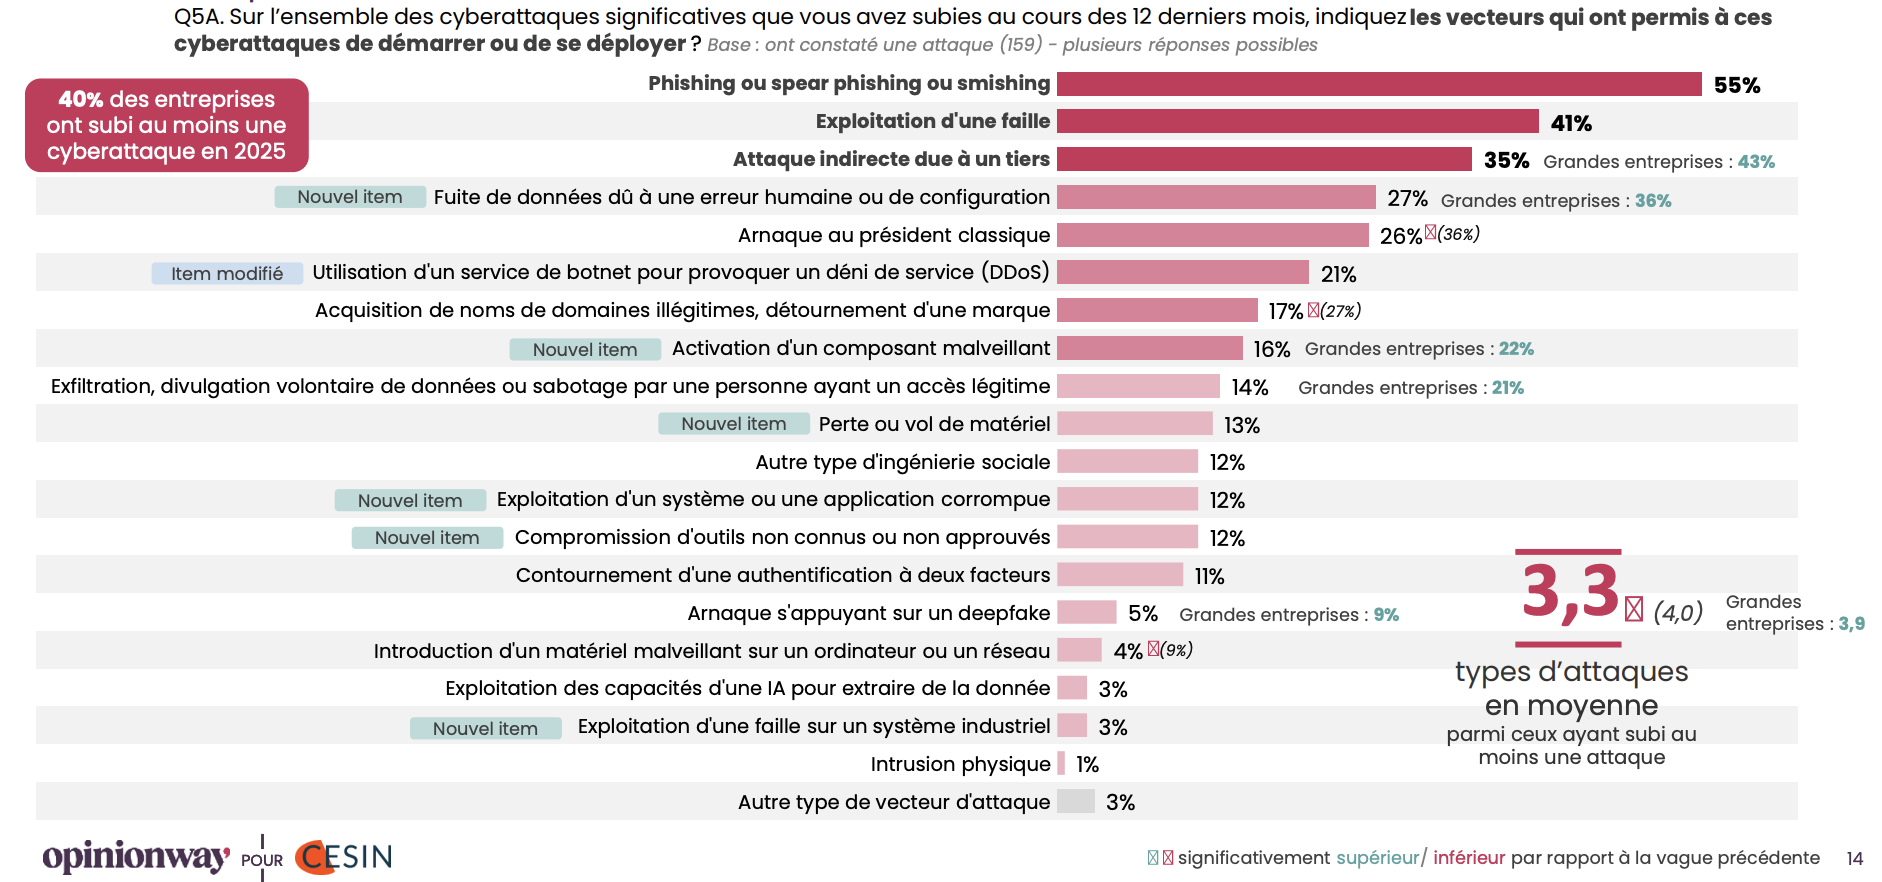
\includegraphics[width=0.80\textwidth]{figures_externes/cesin_2026_vecteurs.png}
\caption{Vecteurs ayant permis aux cyberattaques de démarrer ou de se déployer, exercice $2025$.
Les mentions de droite donnent la part chez les grandes entreprises là où elle diffère
significativement de la moyenne.
Source : baromètre de la cybersécurité des entreprises, OpinionWay pour le CESIN \citep{cesin2026}.}
\label{fig:cesin-vecteurs}
\end{figure}

Une conséquence mérite d'être isolée. La déconnexion par les tiers, c'est-à-dire la mise en
quarantaine de l'entité par ses propres partenaires, est citée dans $12\,\%$ des cas. Elle
renverse le constat précédent : une entité n'est pas seulement atteinte \emph{par} ses
partenaires, elle est aussi coupée \emph{par} eux lorsqu'elle est atteinte. La dépendance joue
dans les deux sens, et les deux sens n'ont ni le même coût ni la même prévention. Aucune mesure
de dépendance symétrique ne peut les distinguer.

\begin{attention}
\textbf{Deux sources qui semblent se contredire, et ne se contredisent pas.} Le baromètre et la
cartographie décrivent un recul de la fréquence, quand le marché assuré affiche un nombre de
sinistres presque triplé (sous-section~\ref{subsec:lucy-freq-sev}). Les deux constats sont
compatibles : le nombre de sinistres du marché est un \emph{total}, porté par une base d'assurés
élargie de $49\,\%$ sur le même exercice, alors que les deux autres sources mesurent une
exposition \emph{par entité}. Un marché peut enregistrer davantage de sinistres tout en assurant
des entités individuellement moins exposées. Confondre le total et la fréquence conduirait à lire
une aggravation là où il y a une extension de périmètre. Ces deux enquêtes sont par ailleurs
déclaratives : elles mesurent ce que les organisations constatent, non ce qui survient.
\end{attention}

\subsection{Les limites de Solvabilité II et de la Formule Standard}
% [etiquette subsec:limites-formule-standard gardee dans le corps]
% HARNAIS-HORS-SECTION: section de cadrage prudentiel, aucune valeur chiffree du projet.

Le risque cyber est donc au premier rang des préoccupations, mesuré par plusieurs sources
indépendantes, et encadré depuis $2025$ par un règlement qui en rend la maîtrise observable.
Aucun dispositif prudentiel ne traduit pourtant ce niveau de maîtrise en capital.

La Formule Standard de Solvabilité~II charge le risque opérationnel par un pourcentage de primes
ou de provisions techniques. Ce forfait est \emph{plat} en conformité : deux entités de bilan
identique et de maturité opposée sur les cinq domaines de DORA acquittent exactement la même
charge. Aucun sous-module cyber n'existe, et le risque couvert par les garanties affirmatives ne
correspond à aucun module standard, ce qui renvoie les assureurs à leurs modèles internes et à
leur évaluation interne des risques et de la solvabilité. L'articulation juridique complète entre
les deux textes est traitée à la section~\ref{chap:reglementaire}.

Les outils actuariels usuels ne comblent pas ce vide. Une copule capturerait la co-occurrence des
pertes entre domaines de contrôle, mais symétriquement : elle ne distingue pas une défaillance
qui \emph{entraîne} les autres d'une défaillance qui les \emph{subit}. Or c'est cette asymétrie
qui devrait commander la priorité de remédiation. Deux matrices de dépendance transposées l'une
de l'autre, que les statistiques usuelles ne permettent pas de distinguer, conduisent à un
capital et à une décision différents : le chapitre~\ref{chap:cascade} le démontre.

% Origine : chapitres_sfe/01_contexte.tex, « Le cadre prudentiel de capital et son articulation avec DORA », deplace le 2026-10-01 (phase 4). Le corps en garde un resume.
\section{Le cadre prudentiel de capital et son articulation avec DORA}
% [etiquette chap:reglementaire gardee dans le corps]

% HARNAIS-HORS-SCRIPT: cadre reglementaire : numeros d'articles, delais de notification et seuils cites des textes (DORA, Solvabilite II, Bale). Ce sont des donnees de droit, pas des resultats.

% MIGRÉ depuis memoire/main.tex (plages 349-617).
% Hiérarchie descendue d'un cran, labels préfixés "reg:".
% RELECTURE FAITE (août 2026). Un résidu de l'ancien modèle a été trouvé et
% corrigé : l'introduction annonçait la non-conformité « comme une variable
% latente », formulation de l'ancien modèle à briques, remplacée par l'état de
% conformité par pilier du ch. 11. Aucune autre phrase du chapitre n'annonce la
% copule ni la latente comme LE modèle.
%==============================================================

Le risque modélisé ici, risque opérationnel d'origine technologique et manquement aux
exigences de résilience numérique, se situe à l'intersection de trois cadres construits
successivement selon des philosophies distinctes : le dispositif bancaire de Bâle, la directive
Solvabilité~II propre à l'assurance, et le règlement transsectoriel DORA. Leur articulation
ouvre un \emph{pont quantitatif} entre exigence de capital et résilience opérationnelle, et
permet de poser la non-conformité comme un état par domaine de contrôle, gradué et évolutif,
dont le chapitre~\ref{chap:multietats} tire la dynamique et le chapitre~\ref{chap:resultats}
le coût en capital.

%--------------------------------------------------------------

%--------------------------------------------------------------

\paragraph{Le risque opérationnel : une définition partagée, des traitements divergents.}
Le risque opérationnel reçoit la même définition dans les secteurs bancaire et
assurantiel. Défini par le Comité de Bâle puis repris par la directive Solvabilité~II,
il désigne le risque de perte résultant de l'inadaptation ou de la défaillance de
procédures internes, de personnels et de systèmes, ou d'événements extérieurs. Cette
définition inclut le risque juridique mais exclut les risques stratégiques et de
réputation.

Si la définition est partagée, les modes de quantification ont divergé. Le secteur bancaire a
abandonné les modèles internes au profit d'une approche standardisée, tandis que l'assurance a
conservé une liberté méthodologique. Cette asymétrie commande le choix méthodologique du
mémoire : Solvabilité~II laisse subsister un espace de modélisation interne, où la
quantification du risque cyber par une distribution de pertes reste recevable.

\paragraph{Bâle III/IV.} Le secteur bancaire a retiré en $2022$ les modèles internes de mesure
avancée au profit d'une approche standardisée, sans invalider l'approche par distribution des
pertes comme outil de modélisation : le mémoire en reprend les deux marges, fréquence et
sévérité, et en remplace l'agrégation par une cascade dirigée. Le détail est déporté
\matcomp.

\paragraph{Solvabilité II : l'asymétrie réglementaire et le maintien du choix méthodologique.}
Contrairement au secteur bancaire, le secteur de l'assurance conserve sous Solvabilité~II
une liberté de choix pour la quantification du risque opérationnel : formule standard,
paramètres propres à l'entreprise (USP), ou modèle interne, partiel ou global, approuvé
par l'autorité de contrôle. Dans la formule standard, l'exigence pour risque opérationnel
($SCR_{Op}$) s'ajoute au capital de solvabilité requis de base
($BSCR$), ajusté de la capacité d'absorption des pertes :
% [environnement reg:eq:scrop garde dans le corps du rapport]
où $Op = \max(Op_{premiums}, Op_{provisions})$ est calculé à partir de coefficients
forfaitaires appliqués aux primes et provisions, vie et non-vie. La forme donnée ici est
simplifiée ; la formule complète de l'Article~204 du règlement délégué~2015/35
comporte en outre des termes de croissance, sous la forme
$\max\!\left(0;\, 0{,}04 \times \Delta\!\right)$, pénalisant les hausses de primes
supérieures à $20\,\%$ d'un exercice à l'autre.

Fondée sur les seuls indicateurs de volume, cette approche pose que deux assureurs gérant le
même volume de primes ont la même exposition au risque opérationnel, quelles que soient la
qualité de leur infrastructure informatique, l'automatisation de leurs processus ou leur
dépendance à des prestataires d'externalisation critiques. C'est cette dépendance
technologique que DORA encadre, et dont le mémoire mesure l'effet sur le capital.

\paragraph{Pilier 1 et Pilier 2.} Le $SCR_{Op}$ relève du Pilier~1, quantitatif et
forfaitaire. Mais Solvabilité~II comporte un second pilier, l'évaluation interne des
risques et de la solvabilité (\emph{Own Risk and Solvency Assessment}, ORSA), qui impose
à l'assureur une évaluation prospective de l'adéquation entre son profil de risque réel
et ses besoins de solvabilité. C'est dans le cadre de l'ORSA, et non du forfait de
Pilier~1 plafonné à $30\,\%$ du $BSCR$, que se situe la modélisation du
mémoire : l'ORSA admet, et encourage, les scénarios de stress stochastiques que la formule
standard ne sait pas produire.

L'additivité que l'équation ci-dessus donne à la charge opérationnelle n'est pas un détail
de présentation. Elle décide de ce que le capital total retient d'un besoin de nature
opérationnelle, et elle le fait dans un sens qui n'est pas neutre pour l'entité : le
\S\ref{sec:agregation-scr} le chiffre sur les quatre bilans réels, et montre que le plafond
lui-même borne ce qu'un forfait saurait exprimer.

\paragraph{DORA, rappelé en une ligne et non réexposé.} Le règlement sur la résilience
opérationnelle numérique du secteur financier, ses cinq domaines de maîtrise et son dispositif de
surveillance des prestataires tiers critiques sont présentés au \S\ref{sec:dora}. Ce chapitre ne
les redit pas : il traite de ce que le chapitre~\ref{chap:cadre-cyber-dora} laisse ouvert, à
savoir l'articulation du règlement avec les exigences de capital qui, elles, préexistent.

\paragraph{Position dans l'écosystème.} La progression Bâle~$\rightarrow$~Solvabilité~II
$\rightarrow$~DORA traduit un déplacement du centre de gravité prudentiel : de la
\emph{couverture financière} du risque (détenir assez de capital) vers la \emph{continuité
opérationnelle} (rester capable d'opérer). DORA ne remplace pas les exigences de capital ;
il en révèle l'angle mort, à savoir la dynamique propre des défaillances technologiques,
que ni le $SCR_{Op}$ forfaitaire ni l'ORSA qualitatif ne savaient capturer.

%--------------------------------------------------------------

%--------------------------------------------------------------

\paragraph{ORSA et DORA.} Les deux cadres partagent un objet, le risque opérationnel d'origine
technologique, et une exigence d'évaluation prospective, mais pas leur finalité : Solvabilité~II
vise la continuité financière, DORA la continuité opérationnelle. La contribution du mémoire se
loge dans leur recouvrement, en utilisant les artefacts produits par DORA pour quantifier dans
l'ORSA ce que celui-ci ne savait que décrire. Les limites de l'ORSA traditionnel, la table
comparative des deux cadres et leurs zones de divergence sont déportées \matcomp.

%--------------------------------------------------------------

% =====================================================================

% Origine : chapitres_sfe/03_donnees.tex, « Cartographie des sources et de leurs rôles », deplace le 2026-10-01 (phase 4). Le corps en garde un resume.
\section{Cartographie des sources et de leurs rôles}
% [etiquette sec:carto gardee dans le corps]
%--------------------------------------------------------------

Aucune base n'est utilisée seule : chaque source alimente une composante précise du modèle,
selon ce qu'elle sait porter.

\begin{center}
\renewcommand{\arraystretch}{1.3}
\begin{tabular}{>{\raggedright}p{3cm} >{\raggedright}p{5.5cm} >{\raggedright\arraybackslash}p{5.5cm}}
\toprule
\rowcolor{lightblue}
\textbf{Source} & \textbf{Rôle dans le modèle} & \textbf{Justification / limite} \\
\midrule
PRC 2025 & Sévérité alternative via conversion Jacobs ; fréquence de référence $\lambda_{ref}$, sans rôle de niveau &
Périmètre défini, mais sévérité dérivée d'un modèle log-log \\
\addlinespace
SAS OpRisk Global & Sévérité (montants réels) et fréquence d'entrée du moteur ($\lambda$) &
Montants observés, mais biais vers les grandes entités financières \\
\addlinespace
Hackmageddon & Parts par vecteur d'attaque (structure du risque) &
Ne fixe aucun niveau : pondère le multiplicateur qui fait passer $\lambda$ d'un état de conformité à l'autre \\
\bottomrule
\end{tabular}
\end{center}

Cette répartition écarte un écueil fréquent : traiter une base généraliste comme si elle
pouvait, seule, calibrer un modèle fréquence-sévérité. Chaque source est mobilisée là où elle
est la plus fiable, et ses limites sont déclarées.

%--------------------------------------------------------------

%--------------------------------------------------------------

L'usage d'un modèle interne, même partiel, est encadré par la directive Solvabilité~II.
L'Article~19 du Règlement Délégué (UE) 2015/35 impose que les données servant au calcul de la
distribution de probabilité prévisionnelle respectent trois critères cumulatifs : exactitude,
exhaustivité et pertinence.

Sur le risque cyber, aucune base publique ou commerciale ne satisfait ces trois critères.
L'actuaire doit donc documenter les biais des données historiques et justifier les
retraitements. La validité du capital calculé ne tient pas à la perfection de la donnée, qui
n'existe pas, mais à la déclaration des limites et à la robustesse du modèle face à ces
biais.

%--------------------------------------------------------------

%--------------------------------------------------------------

% SOURCES-SCRIPTS: 63

% Origine : chapitres_sfe/03_donnees.tex, « Trois biais statistiques à déclarer avant tout usage », deplace le 2026-10-01 (phase 4). Le corps en garde un resume.
\section{Trois biais statistiques à déclarer avant tout usage}
% [etiquette sec:trois-biais gardee dans le corps]

L'utilisation conjointe des bases \emph{Privacy Rights Clearinghouse} (PRC) et SAS OpRisk Global permet de croiser les perspectives, mais nécessite d'identifier trois biais statistiques majeurs qui altèrent l'estimation de l'indice de queue $\xi$.

\paragraph{1. Le biais de sélection (Selection Bias).}
Ce biais affecte particulièrement la base OpRisk Global, qui se nourrit principalement d'événements rendus publics dans la presse financière ou les rapports annuels. Par construction, un incident cyber n'atteint ce seuil de visibilité que s'il frappe une entité d'une certaine taille (généralement des institutions systémiques ou de grandes banques internationales) ou si son montant est exceptionnellement élevé.
Ce biais de taille sur-représente les événements extrêmes et sous-représente la sinistralité
d'attrition. Calibrer directement sur cette base un modèle destiné à une entité de taille
moyenne, une mutuelle régionale par exemple, surestime mécaniquement la probabilité de perte
extrême. C'est pourquoi la fréquence et la sévérité sont ramenées à la taille de l'entité par
deux élasticités estimées (\S\ref{sec:biais-chiffres} et chapitre~\ref{chap:resultats}).

\paragraph{2. Le biais de déclaration (Reporting Bias).}
La base PRC est soumise à un biais de déclaration lié aux asymétries réglementaires. Aux États-Unis, la notification des fuites de données personnelles (Data Breaches) est obligatoire dans la plupart des États, ce qui rend la base PRC très riche sur ce vecteur d'attaque. En revanche, un rançongiciel (Ransomware) qui paralyse les serveurs de l'entreprise mais n'exfiltre aucune donnée personnelle peut ne déclencher aucune obligation de notification légale (avant l'entrée en vigueur d'actes récents comme le CIRCIA).
Calibrer une fréquence globale sur la PRC sous-estime donc le risque d'interruption
d'activité au profit du seul risque de compromission de données. C'est pourquoi la fréquence
qui porte le capital n'est pas lue sur la PRC mais sur OpRisk, qui recense les pertes matérielles
quel que soit le vecteur, et pourquoi la répartition par vecteur, rançongiciels compris, est prise
dans la base Hackmageddon plutôt que dans la PRC.

\paragraph{3. Le biais de survie (Survivorship Bias).}
Dans les bases de pertes opérationnelles, la sévérité maximale observée est paradoxalement bornée par la capacité de survie de l'entité. Une cyberattaque ayant entraîné la faillite pure et simple de l'entreprise (ruine) disparaît souvent des bases de pertes opérationnelles classiques, car il n'y a plus d'entité survivante pour reporter la perte financière finale et les coûts de remédiation à long terme. Ce biais tronque artificiellement l'extrême queue de distribution. La théorie des valeurs
extrêmes ne le corrige pas : une loi de Pareto généralisée ajustée sur un échantillon tronqué
hérite de la troncature, et si elle permet d'extrapoler au-delà du maximum observé, elle le fait
à partir d'une queue allégée. Le biais de survie va donc dans le sens d'une sous-estimation de la
queue, et il s'ajoute aux écarts anti-conservateurs déclarés au chapitre~\ref{ch:robustesse}.

%--------------------------------------------------------------

%--------------------------------------------------------------

% Origine : chapitres_sfe/03_donnees.tex, « L'hétérogénéité temporelle et l'actualisation des sinistres », deplace le 2026-10-01 (phase 4). Le corps en garde un resume.
\section{L'hétérogénéité temporelle et l'actualisation des sinistres}

L'hétérogénéité temporelle des bases de données constitue une autre infraction potentielle au critère d'exactitude de Solvabilité II. La base OpRisk Global agrège des pertes de $2000$ à $2026$. Employer un montant de $2018$ tel
quel dans un modèle de capital de $2026$ fausse le résultat, l'inflation des sinistres
technologiques ne suivant pas l'indice des prix à la consommation.

Le coût d'un sinistre cyber est principalement tiré par trois facteurs :
\begin{itemize}
    \item \textbf{L'inflation salariale IT :} Le coût des experts en remédiation (forensic, restauration de systèmes) connaît une inflation nettement supérieure à l'indice des prix à la consommation, en raison de la pénurie de talents en cybersécurité.
    \item \textbf{L'inflation juridique et réglementaire :} L'entrée en vigueur du RGPD en 2018 a drastiquement modifié l'échelle des sanctions. Une fuite de données en 2015 coûtait infiniment moins cher en amendes administratives que la même fuite en 2025.
    \item \textbf{L'escalade des rançons :} La professionnalisation du cybercrime (Ransomware-as-a-Service) a transformé les demandes de rançons de quelques milliers de dollars en 2016 à plusieurs dizaines de millions d'euros en 2026.
\end{itemize}

Pour respecter les exigences de l'Article 19, les sinistres historiques doivent être actualisés en euros de l'année de modélisation (2026). Soit $L_t$ la perte observée l'année $t$, la perte actualisée $\tilde{L}_{2026}$ s'écrit :
\begin{equation}
\tilde{L}_{2026} = L_t \times \prod_{k=t}^{2025} (1 + i_k^{cyber})
\end{equation}
où $i_k^{cyber}$ est un taux d'inflation propre aux sinistres technologiques, que les indices
sectoriels situent entre $5$ et $10\,\%$ par an. La base OpRisk porte deux montants pour chaque
perte : le montant enregistré l'année de l'événement et sa valeur courante, corrigée de
l'inflation générale. La chaîne publiée lit le premier, donc des montants \emph{nominaux}. Le
rapport entre les deux colonnes vaut un pour les années récentes et $1{,}747$ en $2004$, ce qui
fixe l'inflation implicite à $2{,}19\,\%$ par an. Cette homogénéisation n'est pas appliquée à la
calibration gelée : elle minore les sinistres anciens ramenés en euros courants, donc la queue et
le capital, et son effet sur la dérive des pertes est mesuré au \S\ref{soc:sec:backtest}. Aucun
indice d'inflation spécifique au cyber ne fait aujourd'hui consensus, de sorte que la valeur
courante de la base, fondée sur l'indice général, reste elle-même un minorant de l'actualisation
que l'équation demande.
% SOURCES-SCRIPTS: 102

Par ailleurs, le traitement des données manquantes dans la PRC (qui recense parfois le nombre d'enregistrements compromis sans le montant financier) est géré par la conversion de \citet{jacobs2014}. Bien qu'utile comme \emph{proxy}, ce modèle de régression log-log lisse la variance et minore les extrêmes. C'est le motif de
ne pas plafonner la calibration issue directement d'OpRisk, où les montants sont observés de
bout en bout.

%--------------------------------------------------------------

%--------------------------------------------------------------

Les limites épistémiques et statistiques exposées ci-dessus contraignent aujourd'hui le calcul du SCR cyber à de larges intervalles d'incertitude. Cependant, cette situation est transitoire. L'apport fondamental du règlement DORA ne réside pas uniquement dans l'imposition de normes de sécurité (Chapitre II), mais dans la création d'un cadre de notification harmonisée des incidents majeurs liés aux TIC (Chapitre III, Article 19 de DORA).

DORA impose aux entités financières de reporter à leur autorité compétente (l'ACPR en France) les incidents majeurs selon une taxonomie standardisée (causes, vecteurs, temps de résolution, pertes financières directes et indirectes). À terme, le règlement prévoit la centralisation de ces rapports au sein d'un pôle de l'Union européenne (EU Hub).

Ce registre atténuerait les trois failles actuelles sans les faire disparaître :
\begin{itemize}
    \item \textbf{Biais de déclaration :} la notification étant obligatoire, la base couvrirait
      les incidents \emph{majeurs} au sens du règlement. Elle resterait donc tronquée au seuil
      de matérialité, et non exhaustive : le biais change de nature plutôt qu'il ne disparaît.
    \item \textbf{Biais de sélection :} le registre couvrirait toutes les strates du marché
      financier, courtiers, mutuelles et sociétés de gestion compris, ce qui donnerait la
      granularité nécessaire pour conditionner la sévérité par taille d'entité.
    \item \textbf{Visibilité sur les tiers :} le registre cartographierait l'implication des
      prestataires tiers TIC. C'est exactement la donnée qui manque pour identifier la direction
      de la contagion, et le chapitre~\ref{chap:partielle} chiffre en euros de capital ce que
      son obtention ferait gagner.
\end{itemize}

L'architecture retenue ici (approche par distribution des pertes, théorie des valeurs
extrêmes, facteur de Vasicek, allocation d'Euler) ne dépend pas de la source : le modèle et les
scripts sont agnostiques aux données d'entrée. Substituer une base d'incidents DORA harmonisée
aux bases PRC et OpRisk ne demanderait donc aucune réécriture. Le gain porterait sur la qualité
des entrées, non sur la structure du modèle, et il resterait borné par ce que le registre ne
couvrira pas : les incidents sous le seuil de matérialité, et la direction de la contagion tant
que le registre ne l'horodate pas.

\paragraph{Automatisation du reclassement par NLP.} En attendant ce registre harmonisé, une
partie du travail de fiabilisation peut déjà être outillée. Le reclassement manuel par grille
de mots-clés opéré plus haut sur la taxonomie Hackmageddon, nécessaire pour isoler le
ransomware qui n'existait pas comme catégorie en 2023, illustre une limite récurrente des
bases de sinistralité cyber : une taxonomie déclarative instable, dont la correction repose
sur un travail manuel documenté mais non reproductible à grande échelle.

Les travaux de recherche menés chez Nexialog Consulting sur le traitement automatique du
langage appliqué aux bases de sinistralité cyber (rapports d'incidents, bases de
vulnérabilités, publications techniques) ouvrent une voie pour systématiser ce reclassement.
Le gain serait double : une classification supervisée validée statistiquement remplacerait la
grille ad hoc, et la procédure deviendrait transposable à d'autres bases, OpRisk comme le
futur registre DORA. Faute de corpus annoté dans le périmètre de ce travail, cette piste n'a
pas été mise en \oe uvre ; elle constitue un prolongement direct.

%--------------------------------------------------------------

%--------------------------------------------------------------

La base \emph{Privacy Rights Clearinghouse} (PRC) fournit la fréquence de
référence $\lambda_{ref}$, qui compte des notifications sans seuil de
matérialité et ne porte donc aucun niveau de capital (\S suivante). Son intérêt
tient à son périmètre défini et à sa couverture longitudinale.

La PRC joue toutefois un second rôle, plus fragile : celui de source de
sévérité indirecte, via une conversion dite de Jacobs, qui traduit un nombre
d'enregistrements compromis en un montant de perte financière à partir d'un
modèle log-log. Ce mécanisme permet d'élargir le spectre de tailles
d'incidents disponibles, mais introduit un biais de modèle supplémentaire :
la sévérité qui en résulte n'est pas observée directement, elle est
\emph{dérivée}. La calibration en queue de distribution obtenue sur la PRC,
réalisée en propre sur les 15\,053 incidents 2019--2025 de la base brute,
via la conversion Jacobs $\ln(L) = 7{,}68 + 0{,}76\,\ln(X)$, donne un
paramètre de forme $\hat{\xi}_{\text{PRC}} = 1{,}03$ (IC90\%
$[0{,}97~;~1{,}09]$), caractéristique d'une queue extrêmement lourde, à
espérance infinie, résultat qui, pris seul, rendrait toute simulation
numériquement instable et qui doit donc être lu avec le plafond de sévérité
propre à cette source \matcomp.

La PRC reste utile malgré ces limites parce qu'elle est la seule source
alternative de sévérité : elle éprouve la calibration OpRisk sur un autre
périmètre, sans porter elle-même le niveau.

% SOURCES-SCRIPTS: 57 62 63

% Origine : chapitres_sfe/03_donnees.tex, « Trois fréquences et leur seuil de collecte », deplace le 2026-10-01 (phase 4). Le corps en garde un resume.
\section{Trois fréquences et leur seuil de collecte}

% SOURCES-SCRIPTS: 08b 60 62

\paragraph{Le seuil de collecte et la double lecture de $\lambda$.}
La fréquence est la seule brique du modèle dont la valeur dépende
explicitement du \emph{périmètre de comptage} de la source, et cette dépendance
doit être déclarée avant tout usage du niveau. Un contrôle mené sur le panel
firme-année du SAS OpRisk (sous-catégories TIC, 2005--2022, fenêtre
d'observation propre à chaque firme, de sorte qu'une année sans événement soit
un vrai zéro) donne $0{,}10$ événement par firme et par an toutes firmes
confondues, et $0{,}21$ pour les firmes à au moins dix événements. Ces deux
valeurs sont des \emph{seaux} et ne décrivent aucune entité en particulier : le
chapitre~\ref{chap:resultats} estime $\lambda$ comme une fonction de la taille de
firme et la lit à celle de l'entité visée, ce qui donne $0{,}092$. Toutes trois
sont sans commune mesure avec le taux posé dans le modèle. L'écart n'est pas une erreur de
calage : la base OpRisk ne retient que les pertes au-dessus d'un seuil
de collecte, si bien que le taux qu'on y lit est celui des événements TIC
\emph{matériels}, générateurs d'une perte enregistrée, et non celui de tous les
incidents au sens du reporting DORA. C'est la maille pertinente pour un modèle
de capital, mais elle n'est pas la maille réglementaire, et les deux ne doivent
jamais être comparées terme à terme.

Il en découle une règle de lecture qui vaut pour tout le mémoire. Le taux
$\lambda$ est une propriété d'entité, lisible sur un panel
firme-année ; la charge systémique commune, elle, ne se lit qu'au niveau
\emph{agrégé} et après retrait de tendance, car la surdispersion d'un panel
firme-année est dominée par l'hétérogénéité de taille des firmes, non par un
choc commun. Confondre les deux niveaux d'observation reviendrait à imputer au
risque systémique ce qui n'est qu'un effet de taille. Cette séparation
commande l'interprétation des niveaux de capital du
chapitre~\ref{chap:resultats} : selon l'échelle à laquelle $\lambda$ est lu,
le même modèle décrit un secteur ou une entité, et le
tableau~\ref{tab:echelle} en donne la traduction chiffrée.

\begin{attention}
\textbf{Trois nombres portent le nom de \og{}fréquence\fg{}, et il faut les distinguer une
fois pour toutes.} Le mémoire mobilise trois taux, à trois niveaux d'observation. Les
confondre serait une faute de lecture, et l'on prend donc soin de les nommer séparément.
\begin{center}\small
\renewcommand{\arraystretch}{1.3}
\begin{tabular}{@{}l l r p{5.1cm}@{}}
\toprule
\textbf{Symbole} & \textbf{Source} & \textbf{Valeur} & \textbf{Ce qu'il compte} \\
\midrule
$\lambda_{ref}$ & PRC & $341$/an & notifications de violation de données des
\emph{organisations financières} de la base PRC (code \texttt{BSF}), et non de la base
entière, qui en compte $2\,150$ par an. Sert à \emph{répartir} par vecteur d'attaque, pas à
fixer un niveau de capital. \\
$\lambda$ & OpRisk & $21{,}6$/an & incidents TIC \emph{matériels} du secteur
financier mondial. C'est l'entrée du moteur de cascade et le seul des trois qui
porte le capital. \\
$\lambda_{\text{entité}}$ & OpRisk & $0{,}092$/an & les mêmes incidents matériels, rapportés
à \emph{une} firme et lus \emph{à la taille} de l'entité visée, non dans un seau. C'est
l'échelle de lecture d'une entité soumise à DORA. \\
\bottomrule
\end{tabular}
\end{center}
\vspace{2pt}
Le facteur $3\,719$ entre les extrêmes n'est donc pas une incohérence : c'est l'écart entre
un comptage de notifications, un comptage de pertes matérielles sectorielles et un comptage
de pertes matérielles par entité. Il est recalculé à chaque exécution du pipeline, de sorte
qu'il ne peut plus se désynchroniser des trois fréquences dont il découle.
% SOURCES-SCRIPTS: 67
Seul $\lambda$ alimente le
moteur, et lui
seul doit être invoqué quand le mémoire parle de \og{}la fréquence du modèle\fg{}.
\end{attention}

% Origine : chapitres_sfe/03_donnees.tex, « Deux biais déclarés et leur effet chiffré sur le résultat », deplace le 2026-10-01 (phase 4). Le corps en garde un resume.
\section{Deux biais déclarés et leur effet chiffré sur le résultat}
% [etiquette sec:biais-chiffres gardee dans le corps]

Déclarer un biais ne coûte rien ; le mesurer engage. Les deux limites les plus souvent
opposées à une calibration sur OpRisk, le biais de taille et la troncature à droite, sont
ici chiffrées ; la figure est déportée \matcomp.
% SOURCES-SCRIPTS: 57

\paragraph{Les deux mesures.} Le biais de taille est réel mais faible : corrigée de la troncature
au seuil de collecte, l'élasticité de la sévérité à la taille vaut $b=0{,}087$, et la sévérité
transposée à l'entité notionnelle n'est multipliée que par $0{,}85$. La troncature à droite se
corrige par chain-ladder : les $97$ événements observés sur 2023--2025 deviennent $255$ à
l'ultime, et le risque TIC n'a pas baissé après 2022, il n'est pas encore remonté. Les
régressions, le triangle de développement et la figure sont déportés \matcomp.
% SOURCES-SCRIPTS: 67

\begin{cle}
\textbf{Le résultat qui compte, et qui n'était pas prévisible.} Les deux corrections vont en
sens opposés et se compensent presque exactement sur la perte moyenne :
$0{,}861\times1{,}147=0{,}987$, soit un effet net de $1{,}3\,\%$, inférieur à l'incertitude
d'estimation de chacune prise isolément. Elles ne se compensent pas sur le capital.
À queue lourde, la VaR $99{,}5\,\%$ obéit au principe du grand saut unique : elle répond à la
\emph{sévérité} bien plus qu'à la \emph{fréquence}. La correction de taille agit sur la
sévérité et se transmet donc au quantile ; celle de troncature agit sur la fréquence et s'y
transmet mal. Deux biais qui s'annulent sur l'espérance peuvent ainsi ne pas s'annuler sur le
quantile, et \emph{c'est le quantile qui fait le SCR}. Une compensation constatée en moyenne
n'autorise donc pas à ignorer les deux biais.
\end{cle}

%--------------------------------------------------------------

%--------------------------------------------------------------

% Origine : chapitres_sfe/03_donnees.tex, « Hackmageddon et la structure du risque », deplace le 2026-10-01 (phase 4). Le corps en garde un resume.
\section{Hackmageddon et la structure du risque}
% [etiquette sec:hackmageddon gardee dans le corps]

Cette source a déjà été présentée au \S\ref{sec:carto} comme celle qui porte la
\emph{structure} du risque et non son niveau. Reste à en donner le périmètre exact et les
deux limites qui bornent son usage.

\paragraph{Périmètre consolidé.} Le décompte retenu porte sur le semestre complet et contigu
janvier--juin 2026, soit 1\,041 incidents. La couverture pluriannuelle initialement
envisagée a été abandonnée : l'année 2024 est absente du jeu consulté, et 2025 n'est
disponible que partiellement. La base est donc exploitée pour la \emph{structure} du risque,
non pour son \emph{niveau} ou sa dynamique temporelle : elle ne fixe aucune fréquence, et ses
parts ne servent qu'à pondérer le multiplicateur de fréquence entre états
(\S\ref{sec:quatre-canaux}).

\begin{attention}
\textbf{Ces deux décomptes sont une citation, non un résultat du dispositif.} Contrairement
aux bases PRC et OpRisk, versionnées dans le dépôt du mémoire et rejouables par script, le
jeu Hackmageddon a été consulté puis non conservé. Les $1\,041$ incidents et les
$840$ à vecteur identifié ne sont donc reproductibles par aucun script, et le contrôle de
non-régression du dépôt les signale explicitement comme tels plutôt que de les compter parmi
les sorties vérifiées. Ils sont à lire comme un chiffre de rapport de place, avec sa date de
consultation, et non comme une sortie du modèle. Ces décomptes fixent les parts $\pi_v$ de
répartition par vecteur, qui ne portent aucun niveau mais pondèrent le multiplicateur de
fréquence entre états de conformité (\S\ref{sec:quatre-canaux}) : leur statut de citation
s'étend donc à ce multiplicateur, limite déclarée comme telle. Les faire porter un niveau de
capital serait en revanche indéfendable.

\medskip
\noindent Reste à savoir ce que cette limite coûte, et la réponse est mesurée plus loin dans ce
même chapitre : la catégorie d'un incident \emph{informe} la probabilité qu'il soit lourd, mais
trop faiblement pour porter une segmentation. Trois instruments indépendants le montrent, un $V$
de Cramér sous $0{,}20$, un $\varepsilon^2$ sous $0{,}08$ et des corrélations de rang sous
$0{,}16$ (\S\ref{sec:profilage-variables}). La source la moins traçable du dispositif est donc aussi
celle dont le modèle dépend le moins, et cette coïncidence n'en est pas une : c'est parce que
Hackmageddon ne pouvait pas porter davantage qu'il ne lui a été demandé que cela.
\end{attention}

% Pas de numero : cette section ne porte qu'UN apport, suivi de deux limites. Un
% << Apport 1 >> annoncerait un << Apport 2 >> qui n'existe pas.
\paragraph{Apport : structure du risque et mapping DORA.} Sur les 1\,041
incidents, 840 disposent d'un vecteur d'accès initial identifié (81~\%),
regroupés en familles et reliés directement aux articles DORA :

\begin{center}
\renewcommand{\arraystretch}{1.3}
\begin{tabular}{>{\raggedright}p{5cm} c >{\raggedright\arraybackslash}p{6cm}}
\toprule
\rowcolor{lightblue}
\textbf{Vecteur d'attaque} & \textbf{Part} & \textbf{Exigence DORA} \\
\midrule
Phishing / Ingénierie sociale & 38{,}8~\% & Art.~13, sensibilisation \& formation \\
Exploitation vuln.\ exposée & 33{,}8~\% & Art.~26, tests TLPT ; Art.~8--10 \\
Chaîne d'approvisionnement / tiers TIC & 15{,}8~\% & Art.~28--44, gestion du risque tiers \\
Identifiants compromis & 6{,}3~\% & Art.~9, contrôle d'accès \& MFA \\
\bottomrule
\end{tabular}
\end{center}

Deux chiffres sont structurants pour la construction des scénarios du
chapitre~\ref{chap:multietats} : 15{,}8~\% des attaques empruntent le vecteur tiers/supply
chain, coeur des articles~28--44 ; et 49{,}6~\% relèvent de vecteurs
qu'un test TLPT (art.~26) est censé détecter en amont (exploitation et
tiers cumulés).

\paragraph{Limite 1 : biais de visibilité.} Hackmageddon recense des
incidents rendus publics, majoritairement médiatiques ou déclarés, ce qui
sur-représente structurellement les événements les plus visibles au détriment
des incidents ordinaires, moins commentés. La base ne peut donc servir à
estimer un niveau absolu de fréquence, seulement une répartition relative
entre vecteurs d'attaque.

\paragraph{Limite 2 : taxonomie instable.} Une comparaison de structure entre
2023 (3\,019 incidents, Q3 manquant) et 2026 a mis en évidence un artefact de
taxonomie. La catégorie \og Ransomware\fg{} n'existait pas en 2023, les incidents
correspondants étant alors classés sous \og Malware\fg{}. Une lecture naïve
suggérait une hausse du ransomware de +11 points ; après reclassement par
grille de mots-clés commune, le ransomware \emph{recule} en réalité de
23 points.

\begin{center}
\renewcommand{\arraystretch}{1.3}
\begin{tabular}{>{\raggedright}p{4.5cm} c c c}
\toprule
\rowcolor{lightblue}
\textbf{Dimension} & \textbf{2023} & \textbf{2026} & \textbf{$\Delta$} \\
\midrule
Cybercriminalité (motivation) & 81{,}1~\% & 73{,}9~\% & $-7{,}2$ \\
Cyberespionnage (motivation) & 9{,}6~\% & 20{,}6~\% & $+11{,}0$ \\
Ransomware (reclassé) & 35{,}8~\% & 12{,}7~\% & $-23{,}1$ \\
\bottomrule
\end{tabular}
\end{center}

Seules les motivations (taxonomie stable de haut niveau) sont donc
comparables directement dans le temps ; les types d'attaque ne le
sont qu'après un travail de reclassement documenté. Le signal robuste qui
demeure est la bascule du cybercrime de masse vers l'espionnage ciblé, une
information pertinente pour la discussion du risque systémique au chapitre~\ref{chap:resultats},
mais qui illustre aussi la fragilité méthodologique de toute lecture brute
d'une base de ce type.

% SOURCES-SCRIPTS: 63

%--------------------------------------------------------------

%--------------------------------------------------------------

% Origine : chapitres_sfe/03_donnees.tex, « OpRisk Global et la sévérité en euros », deplace le 2026-10-01 (phase 4). Le corps en garde un resume.
\section{OpRisk Global et la sévérité en euros}
% [etiquette sec:oprisk gardee dans le corps]

% SOURCES-SCRIPTS: 07 47 63

\paragraph{Nature et périmètre.} OpRisk Global est la base de référence
historique du risque opérationnel au sens de Bâle~2/3, comptant
41\,975 incidents après nettoyage d'une aberration de saisie. Le
risque cyber n'y constitue pas une catégorie native : il est reconstruit à
partir des catégories \og Systems Security\fg{} et \og Business Disruption and
System Failures\fg{}. Le périmètre cyber $\times$ finance retenu compte
582 incidents sur la période 2000--2026. La même base porte l'étude des coûts cyber de
\citet{elingwirfs2019}, qui en extraient de même les pertes d'origine informatique.

\paragraph{Lien avec l'approche AMA.} Cette base est historiquement celle
qui alimentait les modèles internes de type \emph{Advanced Measurement
Approach} évoqués à la section~\ref{chap:reglementaire}, avant leur retrait au profit de la SMA sous
Bâle~III/IV. Son usage ici renoue donc, à des fins de modélisation interne et
non de calcul réglementaire de Pilier~1, avec la logique originelle de la LDA
bancaire : calibrer une sévérité extrême à partir de pertes réellement
observées plutôt qu'à partir d'un indicateur de volume forfaitaire.

\paragraph{Statistiques de sévérité.} Elles portent sur la population de la fréquence et de la
descente d'échelle : secteur financier, catégories TIC, fenêtre $2005$--$2022$, soit
$1\,476$ observations. La loi de Pareto généralisée, elle, est ajustée sur le périmètre cyber
$\times$ finance du paragraphe précédent, $582$ pertes sur $2000$--$2026$. Les deux populations
ne coïncident pas, et la table ci-dessous décrit la première.

\begin{center}
\renewcommand{\arraystretch}{1.3}
\begin{tabular}{l r l r}
\toprule
\rowcolor{lightblue}
\textbf{Indicateur} & \textbf{Valeur} & \textbf{Indicateur} & \textbf{Valeur} \\
\midrule
Médiane & 1{,}20 M\$ & P99 & 419{,}3 M\$ \\
Moyenne & 33{,}8 M\$ & Maximum & 10\,970{,}8 M\$ \\
P90 & 25{,}3 M\$ & Total cumulé & 49{,}8 Md\$ \\
\bottomrule
\end{tabular}
\end{center}

La concentration extrême de la sévérité constitue une signature de queue lourde qui justifie
directement le recours à la théorie des valeurs extrêmes développée au
chapitre~\ref{chap:socle} : le décile supérieur porte $92{,}3\,\%$ de la perte totale, et le
seul centile supérieur en porte $65{,}1\,\%$.

% SOURCES-SCRIPTS: 67

\paragraph{Choix du seuil POT.} Le choix du seuil $u$ au-dessus duquel la loi
de Pareto généralisée est calibrée résulte d'un compromis classique
biais-variance, arbitré graphiquement. Le \emph{mean excess plot}
(figure~\ref{don:fig:mep}) présente une pente positive et globalement linéaire
au-delà de $u = 20$~M\euro, signature attendue d'un régime GPD à queue lourde
($\xi > 0$) ; c'est ce seuil, correspondant au percentile~85 de la
distribution des montants, qui est retenu pour la suite.

% [H] et non [htbp] : cette figure derivait jusqu'a la page suivante et coupait en deux le
% paragraphe "La comparaison avec la PRC", qui la suit de deux paragraphes dans le source.
% [H] la fixe a son point d'appel, juste apres le paragraphe qui la commente.
\begin{figure}[H]
\centering
\includegraphics[width=0.70\textwidth]{figures/mean_excess_oprisk.png}
\caption{Mean excess plot sur le périmètre cyber$\times$finance d'OpRisk
Global. La linéarité de $e(u)$ au-delà du seuil retenu $u = 20$~M\euro{}
(pointillés) confirme le régime de queue lourde justifiant l'ajustement GPD.}
\label{don:fig:mep}
\end{figure}

\paragraph{Calibration GPD et validation croisée.} Au seuil du percentile~85
($u = 20{,}0$~M\euro, 91 excès), la calibration GPD donne :
\[
\hat{\xi} = 0{,}595 \quad (\text{IC}_{90\%}=[0{,}30\,;\,0{,}83]), \qquad
\hat{\sigma} = 58{,}0~\text{M\euro}, \qquad
\qsev_{99{,}5\%}(X) = 663~\text{M\euro}.
\]
Le dernier terme est le quantile de la sévérité d'un sinistre, pas un capital : le
besoin de capital est le quantile de la charge \emph{annuelle agrégée}, obtenu plus loin par
composition avec la fréquence. L'intervalle de confiance bootstrap qui entoure ce quantile est
$[411\,;\,1037]$~M\euro, soit un facteur~2{,}5 entre les bornes, une ampleur qui, à elle seule,
illustre que le SCR ne peut être présenté comme un point.

La comparaison avec la PRC ($\hat{\xi}_{\text{PRC}} = 1{,}03$ contre
$\hat{\xi}_{\text{OpRisk}} = 0{,}595$) ne se lit pas comme une différence de
risque, car les deux indices ne portent pas sur le même objet. La sévérité PRC
n'est pas observée : elle est une puissance du nombre d'enregistrements, de
pente $0{,}76$ en logarithme, et une puissance multiplie l'indice de queue par
son exposant, si bien que $\hat{\xi}_{\text{PRC}}$ décrit la queue des
enregistrements transportée en euros. Le biais de taille d'OpRisk, mesuré faible
au \S\ref{sec:biais-chiffres}, n'en rend pas compte. Les deux sources confirment néanmoins le même régime
qualitatif de queue lourde ($\xi > 0$). Il n'existe donc pas de hiérarchie
\og source primaire\fg{} en sévérité : OpRisk fournit des montants réels, la PRC
un spectre de tailles plus large via la conversion Jacobs : deux
estimations indépendantes et complémentaires, dont l'écart constitue
lui-même une information sur l'incertitude du modèle.

La décomposition par sous-catégorie révèle en outre deux profils de risque
distincts : les pannes (\og Business Disruption\fg{}) sont moins fréquentes
(19~\% des incidents) mais nettement plus coûteuses, avec une médiane cinq
fois supérieure à celle des intrusions (\og Systems Security\fg{}), suggérant que
les multiplicateurs DORA pourraient à terme être différenciés non seulement
en fréquence mais aussi en sévérité, sous réserve de la taille réduite de
l'échantillon \og pannes\fg{} (28 excès), qui rend cette calibration indicative.

%--------------------------------------------------------------

%--------------------------------------------------------------


%--------------------------------------------------------------

% Origine : chapitres_sfe/03_donnees.tex, « Analyse exploratoire, tests statistiques et profilage des variables », deplace le 2026-10-01 (phase 4). Le corps en garde un resume.
\section{Analyse exploratoire, tests statistiques et profilage des variables}
% [etiquette sec:profilage-variables gardee dans le corps]
%--------------------------------------------------------------
% SOURCES-SCRIPTS: 104

Les deux sources viennent d'être décrites par leur périmètre et par leurs biais. Elles ne
l'ont pas été par leurs \emph{variables} : ni le type de chacune, ni son taux de renseignement,
ni la moindre mesure d'association entre elles. Cette section comble ce manque, et elle le fait
dans l'ordre où la question se pose à un lecteur prudentiel. Quelle information chaque base
porte-t-elle réellement ? Sur quelle part de ses lignes ? Et cette information segmente-t-elle
la perte assez nettement pour qu'un modèle ait intérêt à en tenir compte ?

La réponse à la troisième question commande un choix de modélisation qui engage tout le
document, celui d'ajuster une queue \emph{commune} plutôt qu'une queue par catégorie
d'organisation ou par type d'incident.

\subsection{Les variables retenues et leur taux de renseignement}
\label{subsec:table-variables}
% SOURCES-SCRIPTS: 104

\paragraph{Un piège de complétude, et il fausse la lecture dans le bon sens pour qui ne le voit
pas.} Dans l'export de la chronologie PRC, un champ non renseigné ne vaut pas vide : il vaut la
chaîne \texttt{UNKN}. Un contrôle de complétude ordinaire, qui teste l'absence de valeur, rend
donc $100\,\%$ de présence sur les trente-sept colonnes, y compris sur celles qui ne sont
documentées que dans un cas sur quatre. Les taux ci-dessous comptent \texttt{UNKN} comme un
manquant, ce qui est le seul comptage défendable, et le script imprime les deux mesures côte à
côte pour que l'écart soit visible plutôt que supposé.

\begin{center}\small
\renewcommand{\arraystretch}{1.15}
\begin{tabular}{@{}l l p{4.6cm} l r@{}}
\toprule
\textbf{Variable} & \textbf{Type} & \textbf{Rôle dans le modèle} & \textbf{Base} &
\textbf{Renseignée} \\
\midrule
\texttt{total\_affected}      & quantitative & volume d'enregistrements touchés, seule mesure
                                               d'impact de la base & PRC & $41{,}77\,\%$ \\
\texttt{residents\_affected}  & quantitative & sous-ensemble territorialisé du précédent
                                             & PRC & $79{,}88\,\%$ \\
\texttt{breach\_date}         & temporelle   & date de survenance, support de la fréquence annuelle
                                             & PRC & $54{,}82\,\%$ \\
\texttt{reported\_date}       & temporelle   & date de notification, support du délai de détection
                                             & PRC & $99{,}54\,\%$ \\
\texttt{end\_breach\_date}    & temporelle   & fin d'exposition, support de la durée d'incident
                                             & PRC & $28{,}18\,\%$ \\
\texttt{organization\_type}   & qualitative  & classe d'organisation, huit modalités
                                             & PRC & $89{,}29\,\%$ \\
\texttt{breach\_type}         & qualitative  & vecteur de la brèche, huit modalités
                                             & PRC & $47{,}31\,\%$ \\
\midrule
\texttt{Loss Amount}          & quantitative & montant de perte avérée, source de la sévérité
                                             & SAS & $100\,\%$ \\
\texttt{Event Risk Category}  & qualitative  & catégorie bâloise de niveau 1, sept modalités
                                             & SAS & $100\,\%$ \\
\texttt{Sub Risk Category}    & qualitative  & sous-catégorie, définit le périmètre TIC
                                             & SAS & $100\,\%$ \\
\texttt{Basel Business Line}  & qualitative  & ligne métier, dix modalités
                                             & SAS & $100\,\%$ \\
\texttt{Industry Sector Name} & qualitative  & secteur, définit le périmètre financier
                                             & SAS & $100\,\%$ \\
\texttt{Revenue}              & quantitative & chiffre d'affaires, mesure de taille
                                             & SAS & $87{,}82\,\%$ \\
\texttt{Assets}               & quantitative & actif total, mesure de taille prudentielle
                                             & SAS & $83{,}51\,\%$ \\
\bottomrule
\end{tabular}
\end{center}

\vspace{2pt}
\noindent\textbf{Lecture.} La chronologie PRC porte $74\,783$ incidents, dont $31\,217$ seulement
documentent un volume touché strictement positif. Après restriction à la période retenue,
$15\,053$ incidents subsistent, effectif que ce recomptage indépendant retrouve à l'unité près
sur les sorties déjà versionnées du projet. La base SAS porte $41\,976$ lignes, dont $41\,975$
pertes exploitables ; le périmètre TIC en compte $1\,099$ et son intersection avec le secteur
financier $582$.

% SOURCES-SCRIPTS: 104

\begin{attention}
\textbf{La variable d'impact est la moins bien renseignée des deux bases, sans que ce soit un
hasard de collecte.} Les champs qu'une obligation de notification impose, la date de déclaration
et la nature de l'organisation, sont documentés ; ceux qui demandent une investigation, le volume
touché et la date réelle de survenance, ne le sont pas. Le manquant n'est donc pas aléatoire : il
est corrélé à la difficulté de l'enquête, donc plausiblement à la gravité.

\textbf{Ce mécanisme n'est aucun des trois biais de la section~\ref{sec:trois-biais}, et il se
distingue du deuxième.} Le biais de déclaration porte sur les incidents qui \emph{entrent} dans la
base, selon que la loi impose ou non de les notifier ; celui-ci porte sur les champs
\emph{renseignés} au sein des incidents déjà entrés. Les deux vont dans le même sens et
s'ajoutent, mais ils opèrent à deux niveaux distincts, et seul le second se mesure sur les
variables au lieu de s'argumenter.
\end{attention}

\begin{figure}[htbp]
\centering
\begin{subfigure}{0.49\textwidth}
  \centering
  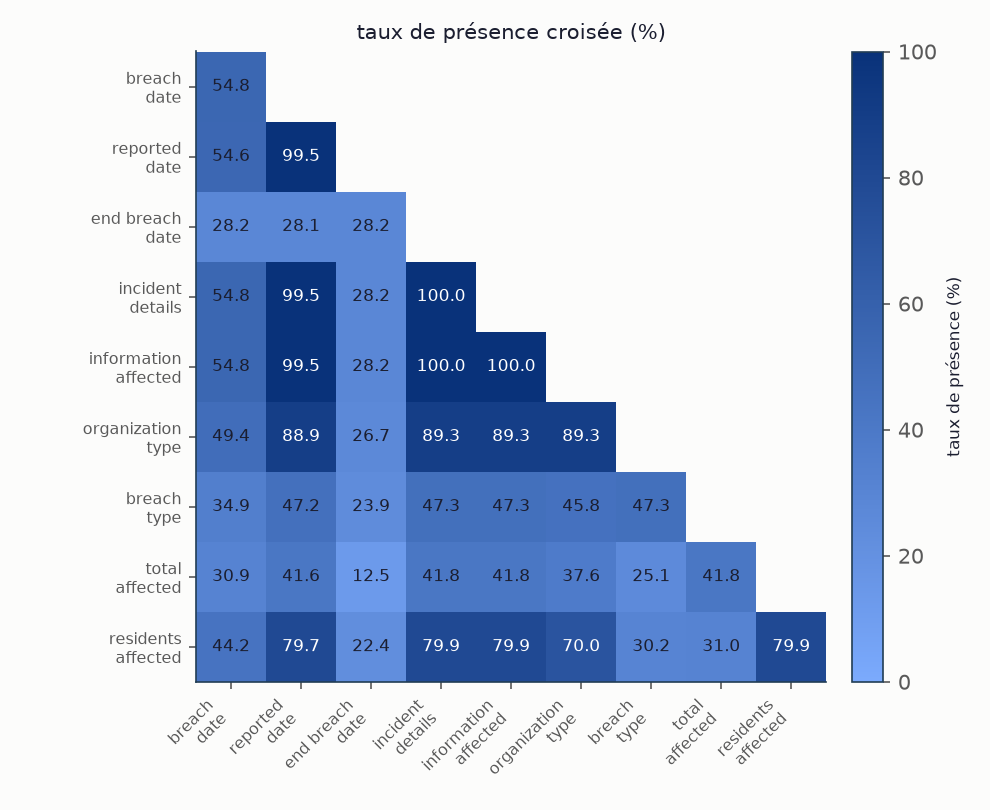
\includegraphics[width=\linewidth]{../recherche/vasicek_lab/figures/D1a_presence_taux.png}
  \caption{}\label{fig:presence-taux}
\end{subfigure}\hfill
\begin{subfigure}{0.49\textwidth}
  \centering
  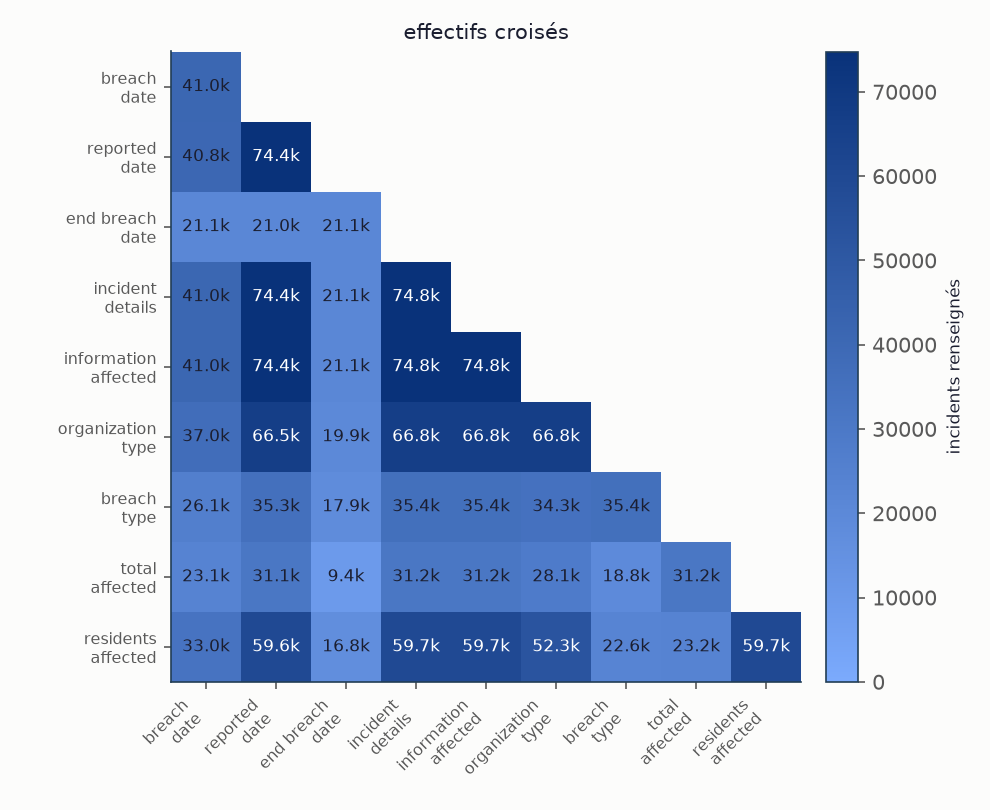
\includegraphics[width=\linewidth]{../recherche/vasicek_lab/figures/D1b_presence_effectifs.png}
  \caption{}\label{fig:presence-effectifs}
\end{subfigure}
\caption{Présence croisée des variables de la chronologie PRC, en taux (a) et en effectifs (b).
La lecture utile est la ligne du bas du panneau (a) : le volume touché n'est simultanément
renseigné avec le type de brèche que dans $25{,}1\,\%$ des cas, et avec la date de fin
d'exposition dans $12{,}5\,\%$. Le panneau (b) donne l'effectif derrière chaque taux.}
\label{fig:presence-croisee}
\end{figure}

Les deux panneaux de la figure~\ref{fig:presence-croisee} ne disent pas la même chose et il faut
les lire ensemble : un taux ne dit pas sur quel effectif il porte. Les $12{,}5\,\%$ du croisement le plus pauvre représentent encore
plus de neuf mille incidents, ce qui n'a pas la même portée qu'un taux identique sur une base de
quelques centaines. La matrice dit surtout ce qu'une colonne de taux isolés ne dit pas : les
lacunes se \emph{cumulent}. Une analyse qui croiserait le volume touché, le type de brèche et la durée
d'exposition ne disposerait plus que de $10{,}9\,\%$ de la base, et cette fraction n'aurait aucune
raison d'en être représentative, les trois manques ayant la même origine. C'est le motif pour lequel le modèle ne conditionne la sévérité
sur aucune de ces variables.

\subsection{Description des variables d'impact}
\label{subsec:describe-impact}
% SOURCES-SCRIPTS: 104

Le mémoire publie des quantiles de sévérité dans plusieurs chapitres sans les avoir jamais
rassemblés : un lecteur qui veut juger la queue avant de lire l'ajustement devait les
reconstituer de proche en proche. La table ci-dessous les réunit sur les quatre variables
d'impact du dispositif.

\begin{center}\small
\renewcommand{\arraystretch}{1.1}
\begin{tabular}{@{}l r r r r@{}}
\toprule
& \multicolumn{2}{c}{\textbf{PRC}} & \multicolumn{2}{c}{\textbf{SAS OpRisk}} \\
\cmidrule(lr){2-3}\cmidrule(lr){4-5}
& \textbf{enregistrements} & \textbf{sévérité dérivée} & \textbf{toutes catég.} &
\textbf{cyber $\times$ finance} \\
& (nombre) & (M\euro) & (M\euro) & (M\euro) \\
\midrule
$n$              & $15\,053$     & $15\,053$   & $41\,975$  & $582$ \\
moyenne          & $102\,646$    & $6{,}07$    & $69{,}98$  & $24{,}32$ \\
écart-type       & $1\,235\,098$ & $41{,}59$   & $647{,}26$ & $97{,}71$ \\
minimum          & $1$           & $0{,}0020$  & $0{,}0920$ & $0{,}0920$ \\
\midrule
$q_{25}$         & $69$          & $0{,}0497$  & $1{,}012$  & $0{,}352$ \\
médiane          & $1\,104$      & $0{,}409$   & $3{,}763$  & $1{,}380$ \\
$q_{75}$         & $8\,330$      & $1{,}901$   & $18{,}40$  & $8{,}625$ \\
$q_{85}$         & $23\,467$     & $4{,}176$   & $45{,}40$  & $22{,}03$ \\
$q_{90}$         & $49\,000$     & $7{,}307$   & $82{,}90$  & $47{,}42$ \\
$q_{95}$         & $164\,673$    & $18{,}36$   & $202{,}4$  & $105{,}4$ \\
$q_{99}$         & $1\,719\,753$ & $109{,}2$   & $1\,012$   & $369{,}7$ \\
maximum          & $60\,000\,000$& $1\,624$    & $53\,360$  & $1\,380$ \\
\midrule
$q_{99}/$médiane & $1\,558$      & $267$       & $269$      & $268$ \\
maximum$/q_{99}$ & $34{,}9$      & $14{,}9$    & $52{,}7$   & $3{,}7$ \\
coef. de variation & $12{,}03$   & $6{,}85$    & $9{,}25$   & $4{,}02$ \\
\bottomrule
\end{tabular}
\end{center}

\vspace{2pt}
\noindent\textbf{Lecture.} Les deux premières colonnes comptent des enregistrements, les deux
dernières des euros : elles ne se comparent ni en niveau ni en quantile. La quatrième est celle
qui porte la calibration publiée. Trois traits s'y lisent d'un coup.

\begin{itemize}[leftmargin=1.4em,itemsep=3pt]
\item \textbf{La moyenne dépasse le troisième quartile sur les quatre colonnes.} Une
      distribution dont la moyenne tombe au-dessus du $q_{75}$ n'est pas décrite par sa moyenne :
      son niveau est porté par une minorité d'observations.
\item \textbf{Le rapport du $q_{99}$ à la médiane} vaut près de $270$ sur les trois colonnes
      monétaires et monte à $1\,558$ sur les enregistrements. Ce n'est pas une queue qui se
      prolonge, c'est une queue qui change d'échelle.
\item \textbf{Le coefficient de variation} vaut $4{,}02$ sur le périmètre calibré et jusqu'à
      $12{,}03$ sur les enregistrements. Une loi exponentielle le vaut exactement un.
\end{itemize}

% SOURCES-SCRIPTS: 104

\begin{attention}
\textbf{Une asymétrie entre les deux dernières colonnes, à ne pas lire de travers.} Le rapport
du maximum au $q_{99}$ vaut $3{,}7$ sur le périmètre cyber $\times$ finance contre $52{,}7$ sur
la base entière. Le périmètre retenu est donc le \emph{moins} extrême des deux en ce sens, et non
le plus : le sinistre le plus lourd du fichier ne relève pas du risque informatique. La queue
calibrée n'est pas celle de l'événement le plus spectaculaire de la base, ce qui écarte le
soupçon d'un ajustement tiré par un cas isolé.
\end{attention}

\paragraph{Un repère de seuil, et le contrôle qu'il permet.} Le $q_{85}$ du périmètre calibré
vaut $22{,}03$~M\euro{} sur la donnée courante, quand le seuil publié et gelé vaut
$20{,}03$~M\euro, soit le percentile $84{,}4$. L'écart est attendu et il est la trace du gel : il
avait fait diverger trois scripts de validation tant qu'ils redérivaient leur propre seuil au
lieu de le lire dans la configuration. Le contrôle qui vaut porte donc sur le \emph{nombre
d'excès} au-dessus du seuil publié, et il en compte $91$, exactement l'effectif que la
calibration déclare.

\subsection{Les plus gros incidents}
\label{subsec:top-incidents}
% SOURCES-SCRIPTS: 104

Une queue lourde reste une abstraction tant qu'on ne voit pas les événements qui la forment.
La table ci-dessous montre les plus gros incidents de la chronologie PRC, comptés en
enregistrements : elle illustre la forme d'une telle queue, non le quantile publié, calibré en
euros sur OpRisk.

\begin{center}\footnotesize
\renewcommand{\arraystretch}{1.08}
\begin{tabular}{@{}l l l r@{}}
\toprule
\textbf{Organisation} & \textbf{Secteur} & \textbf{Survenance} &
\textbf{Enregistrements} \\
\midrule
Progress Software, Ipswitch, Inc.     & services & 2023-05-27 & $60\,000\,000$ \\
T-Mobile USA, Inc.                    & services & 2021-08-13 & $53\,700\,000$ \\
AT\&T Inc.                            & services & 2024-03-26 & $51\,226\,382$ \\
Logan Health Medical Center           & santé    & 2021-11-22 & $40\,000\,000$ \\
T-Mobile                              & services & 2022-11-25 & $37\,000\,000$ \\
Comcast Cable Communications LLC      & services & 2023-10-16 & $35\,879\,455$ \\
Zoosk, Inc.                           & services & 2020-01-12 & $24\,200\,000$ \\
CafePress, Inc.                       & détail   & 2019-02-19 & $23\,000\,000$ \\
Texas Dow Employees Credit Union      & finance  & 2023-05-29 & $20\,000\,000$ \\
Evite, Inc.                           & services & 2019-02-22 & $18\,571\,486$ \\
loanDepot.com, LLC                    & finance  & 2024-01-03 & $16\,924\,071$ \\
ClearVoiceResearch.com, LLC           & services & 2021-04-16 & $15\,700\,000$ \\
\bottomrule
\end{tabular}
\end{center}

\vspace{2pt}
\noindent\textbf{Lecture.} Le premier incident est la compromission du logiciel de transfert de
fichiers évoquée au chapitre~\ref{chap:cadre-cyber-dora} comme choc de cause commune : il figure
ici sous le nom de l'éditeur du logiciel, et non sous ceux des milliers d'organisations atteintes
à travers lui. Deux entrées distinctes portent le même opérateur de télécommunications à deux
années d'intervalle. Les deux incidents financiers, un établissement de crédit et un prêteur
hypothécaire, dépassent chacun quinze millions d'enregistrements.

% SOURCES-SCRIPTS: 104

\paragraph{La concentration, mesurée : l'argument de queue rendu concret.} La moitié du
volume de sept années tient dans $31$ incidents sur $13\,410$, soit $0{,}23\,\%$ de la
base. Quatre-vingts pour cent tiennent dans $209$ incidents et quatre-vingt-dix pour cent dans
$491$. Un modèle qui décrirait cette distribution par son centre manquerait donc son objet : le
niveau n'est pas produit par le régime courant, il est produit par une poignée d'événements.
C'est ce que l'ajustement par dépassement de seuil formalise, et c'est aussi pourquoi le
quantile qui porte le besoin de capital est porté par un sinistre unique plutôt que par une
accumulation.

\begin{attention}
\textbf{Un défaut de la base, trouvé en regardant cette table et non en relisant une
documentation.} La chronologie PRC n'agrège pas les notifications : un même incident déclaré à
plusieurs autorités y figure autant de fois, avec le même volume. La table brute affichait ainsi
un même établissement de crédit \emph{quatre} fois. Une déduplication sur le triplet
organisation, volume et date de survenance retire $1\,643$ lignes, soit $10{,}9\,\%$ de la
période retenue.

Ce chiffre est une \emph{borne basse} : la déduplication exige une égalité exacte, donc elle ne
rapproche ni deux graphies d'une même raison sociale, ni deux notifications décalées d'un jour.
Des doublons résiduels subsistent et restent visibles ci-dessus. Les traiter demanderait un
appariement approximatif dont le taux d'erreur serait lui-même à estimer.

\textbf{Le mémoire n'est pas affecté}, et le motif est précis : il n'additionne jamais ces
volumes pour produire un montant. Il les utilise comme un échantillon de sévérité, où chaque
ligne est une observation. La réserve vaut pour qui reprendrait la base à d'autres fins, et elle
est déclarée ici plutôt que laissée à découvrir.
\end{attention}

\paragraph{La profondeur de collecte, montrée plutôt que déclarée.} Le mémoire borne sa fenêtre
d'observation au motif que la base ne couvre pas les années anciennes. L'affirmation était
écrite, elle n'était pas visible. Elle l'est ici : avant $2015$, la chronologie ne porte que
$2\,152$ incidents, soit $6{,}5\,\%$ de la période $2005$--$2025$. Le maximum est atteint en
$2023$ avec $5\,866$ incidents, et l'exercice $2025$ n'en compte que $174$, soit $3{,}0\,\%$ du
pic, faute de notifications déjà enregistrées (figure~\ref{fig:composition-temporelle}).

\begin{figure}[htbp]
\centering
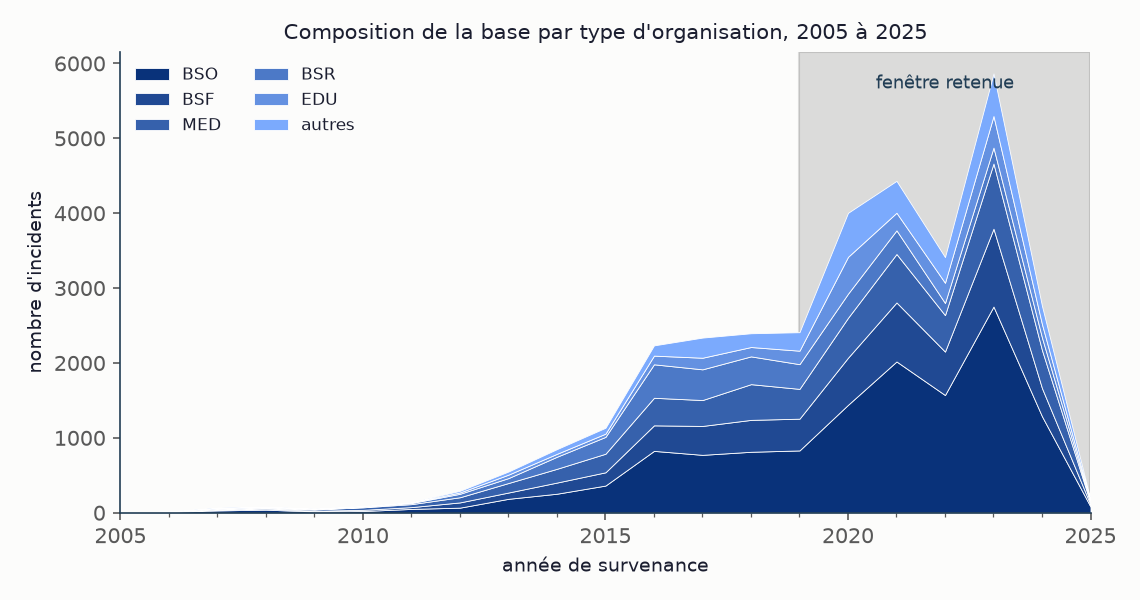
\includegraphics[width=0.92\textwidth]{../recherche/vasicek_lab/figures/D4_composition_temporelle.png}
\caption{Composition de la chronologie PRC par type d'organisation et par année. La zone grisée
est la fenêtre retenue. La montée d'avant $2019$ est une montée de la \emph{collecte}, pas du
risque ; la chute de $2025$ est un défaut de recul, pas une accalmie.}
\label{fig:composition-temporelle}
\end{figure}

Ces deux déformations vont en sens contraire et aucune n'est un signal de risque. Une fenêtre
plus large fabriquerait un régime calme au début et un effondrement à la fin, et un modèle de
tendance ajusté dessus mesurerait la maturation d'une base de données. C'est le motif, déjà
retenu pour la validation hors échantillon, de s'en tenir à la fenêtre grisée.

\paragraph{Compter et sommer ne classent pas les mêmes catégories.} La
figure~\ref{fig:organisation-double-axe} met en regard le nombre d'incidents et le volume touché
par type d'organisation. Les deux ordres divergent sur quatre types sur sept : le
commerce de détail est sixième en nombre et quatrième en volume, l'enseignement quatrième en
nombre et cinquième en volume.

\begin{figure}[htbp]
\centering
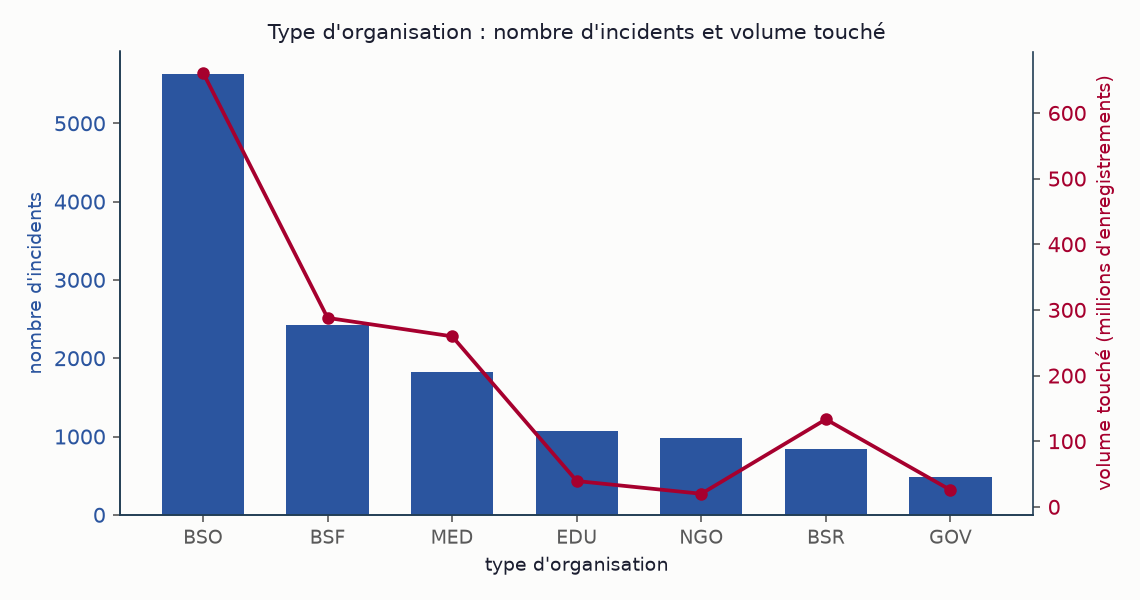
\includegraphics[width=0.92\textwidth]{../recherche/vasicek_lab/figures/D5_organisation_double_axe.png}
\caption{Nombre d'incidents en barres et volume touché en courbe, par type d'organisation. Les
deux classements ne coïncident pas.}
\label{fig:organisation-double-axe}
\end{figure}

C'est la traduction visuelle du résultat de la sous-section~\ref{subsec:tests-qualitatifs} : la
classe d'organisation informe la sévérité sans la déterminer. Un indicateur qui mêlerait
fréquence et volume classerait donc les catégories dans un ordre qu'aucune des deux mesures ne
soutient seule.

\subsection{Association des variables qualitatives au dépassement du seuil}
\label{subsec:tests-qualitatifs}
% SOURCES-SCRIPTS: 104

La question posée est celle d'un actuaire qui envisage de segmenter : le type d'incident ou la
classe d'organisation prédisent-ils qu'une perte dépasse un seuil élevé ? On binarise donc
l'impact au troisième quartile de chaque base, $8\,330$ enregistrements pour la PRC et
$20{,}00$~M\$ pour SAS, puis l'on teste l'indépendance par un $\chi^2$ et l'on mesure la force du
lien par un $V$ de Cramér à correction de Bergsma.

\begin{center}\small
\renewcommand{\arraystretch}{1.15}
\begin{tabular}{@{}l l r r r@{}}
\toprule
\textbf{Base} & \textbf{Variable croisée au dépassement} & \textbf{$\chi^2$} & \textbf{ddl} &
\textbf{$V$ de Cramér} \\
\midrule
PRC & type de brèche              & $43{,}1$     & $6$  & $0{,}068$ \\
PRC & type d'organisation         & $296{,}4$    & $6$  & $0{,}148$ \\
\midrule
SAS & catégorie bâloise           & $1\,301{,}9$ & $6$  & $0{,}176$ \\
SAS & ligne métier bâloise        & $1\,238{,}5$ & $9$  & $0{,}171$ \\
SAS & secteur d'activité          & $711{,}9$    & $20$ & $0{,}128$ \\
\bottomrule
\end{tabular}
\end{center}

\vspace{2pt}
\noindent\textbf{Lecture.} Les cinq tests rejettent l'indépendance, et ce rejet n'apprend rien.
À quinze mille et quarante mille observations, le $\chi^2$ détecte des écarts sans portée
pratique : sa p-valeur mesure l'effectif autant que l'association. Le renseignement est dans le
$V$, qui est une taille d'effet bornée par un et ne croît pas avec $n$. Aucune des cinq
associations n'atteint $0{,}20$, quand $0{,}30$ marque conventionnellement le seuil d'une
association moyenne. La plus forte, la catégorie bâloise dans SAS, vaut $0{,}176$.

% SOURCES-SCRIPTS: 104

\begin{cle}
\textbf{Ce que ces cinq nombres autorisent, et ce qu'ils interdisent.} Ils autorisent à dire que
la catégorie d'un incident \emph{informe} la probabilité qu'il soit lourd. Ils interdisent d'en
faire une variable de segmentation : une association de $0{,}18$ ne porte pas un ajustement de queue par
modalité : segmenter par la catégorie bâloise, qui compte sept modalités, ramènerait les $91$
excès de la calibration à une douzaine par modalité, effectif sur lequel aucune loi de queue ne
s'ajuste. C'est le premier des deux arguments qui fondent le choix d'une queue commune.
\end{cle}

\subsection{Forme, dépendance de rang et hétérogénéité des variables quantitatives}
\label{subsec:tests-quantitatifs}
% SOURCES-SCRIPTS: 104

\paragraph{La normalité, chiffrée plutôt qu'écartée d'un mot.} Le test de Shapiro-Wilk est
appliqué à l'échelle brute puis à l'échelle logarithmique, sur un tirage plafonné à $5\,000$
observations, graine fixée, la statistique n'étant pas fiable au-delà. À l'échelle brute, la
statistique $W$ vaut $0{,}037$ sur la PRC et $0{,}071$ sur SAS, pour une valeur de référence de
un : le rejet est total. Les moments le confirment, avec une asymétrie de $29{,}4$ et un
aplatissement de $1\,083$ sur la PRC, contre trois pour une loi normale.

Le passage au logarithme améliore nettement la statistique sans la sauver, $W$ montant à
$0{,}970$ et $0{,}986$. C'est exactement le diagnostic attendu : la perte n'est ni normale ni
tout à fait log-normale, sa queue restant plus lourde qu'une log-normale ne l'admet. Cette
mesure justifie le recours à une loi de Pareto généralisée \emph{au-delà d'un seuil} plutôt
qu'à un ajustement paramétrique global, choix que la section de calibration met en \oe uvre.

\paragraph{La perte suit mal la taille : un second chemin le mesure.} Les
corrélations de rang de Spearman entre le montant de perte et les trois mesures de taille
disponibles valent $0{,}159$ pour le chiffre d'affaires, $0{,}139$ pour l'effectif et $0{,}068$
pour l'actif total, sur $33\,769$ pertes à profil financier complet. Une perte proportionnelle à
la taille donnerait un coefficient proche de un.

\begin{attention}
\textbf{La mesure de taille la moins liée à la perte est celle qui sert à l'échelle
prudentielle.} L'actif total arrive dernier des trois prédicteurs, derrière le chiffre d'affaires
et derrière l'effectif. Or c'est le bilan qui porte la mise à l'échelle du besoin de capital. Ce
constat, obtenu sans hypothèse de forme et sur un effectif dix fois supérieur à celui de la
descente d'échelle, va dans le même sens que l'élasticité de $0{,}087$ mesurée par ailleurs : il
ne la confirme pas au sens statistique, les deux grandeurs n'étant pas la même, mais il rend
cette faible élasticité moins surprenante. Elle corrobore par un chemin indépendant la limite
\emph{sévérité non plafonnée à l'échelle d'entité}, inscrite au registre des limites du
chapitre~\ref{ch:robustesse}, et c'est cette limite qui fait lire le besoin de capital de
l'entité notionnelle comme une borne supérieure d'ordre de grandeur plutôt que comme une mesure.
\end{attention}

\paragraph{L'hétérogénéité entre classes existe, mais elle est petite.} Le test de Kruskal-Wallis,
non paramétrique donc insensible à la non-normalité qui vient d'être établie, rejette l'égalité
des distributions de sévérité entre classes dans les quatre configurations testées. La taille
d'effet $\varepsilon^2$ dit de combien : $0{,}0100$ pour le type d'organisation et $0{,}0123$ pour
le type de brèche dans la PRC, $0{,}0720$ pour la catégorie bâloise et $0{,}0785$ pour la ligne
métier dans SAS. La classe explique donc entre un et huit pour cent de la dispersion des
sévérités.

% SOURCES-SCRIPTS: 104

% [H] : en [htbp] cette figure derivait en tete de la page suivante et s'inserait entre les deux
% moitiees du mot << contre-disent >> du paragraphe ci-dessous. Fixee ici, elle ouvre la page et
% le paragraphe la suit entier.
\begin{figure}[H]
\centering
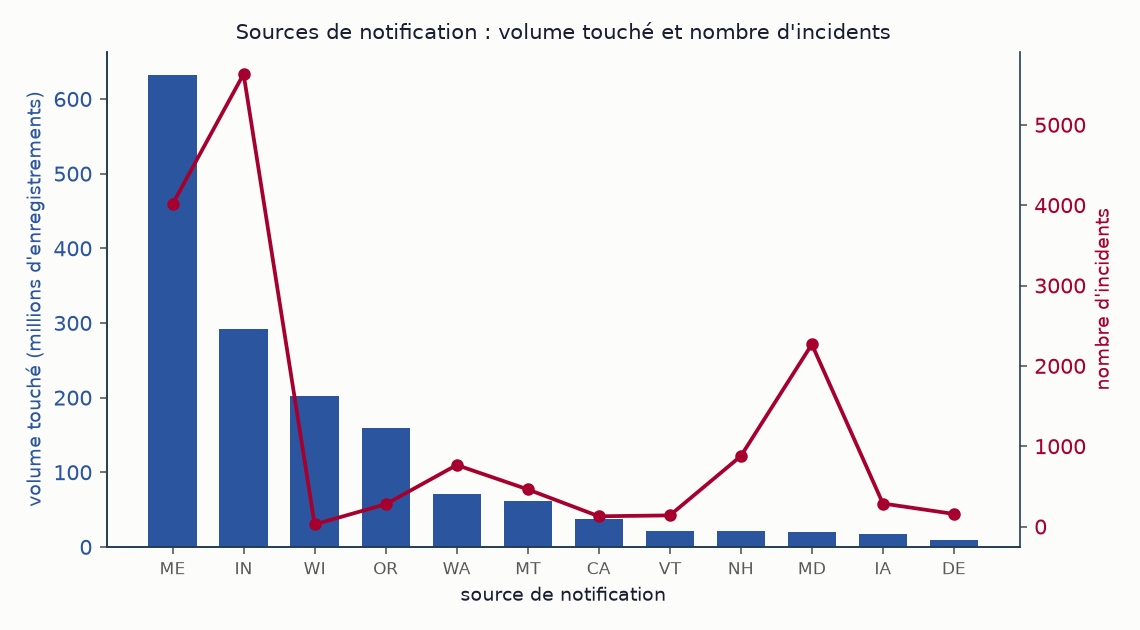
\includegraphics[width=0.90\textwidth]{../recherche/vasicek_lab/figures/D2_sources_notification.png}
\caption{Sources de notification de la chronologie PRC : volume touché en barres, nombre
d'incidents en courbe. Les deux ordres ne coïncident pas.}
\label{fig:sources-notification}
\end{figure}

La figure~\ref{fig:sources-notification} porte un avertissement de méthode plus qu'un résultat.
Les deux axes se contredisent : la source la plus prolixe en nombre d'incidents n'est pas celle
qui porte le plus gros volume, et une source ne déclarant que vingt-sept incidents en concentre
plus de deux cents millions d'enregistrements. Compter les incidents et sommer les volumes
répondent donc à deux questions différentes, et un indicateur agrégé qui mêlerait les deux
serait dominé par le régime déclaratif de quelques juridictions.

\begin{figure}[htbp]
\centering
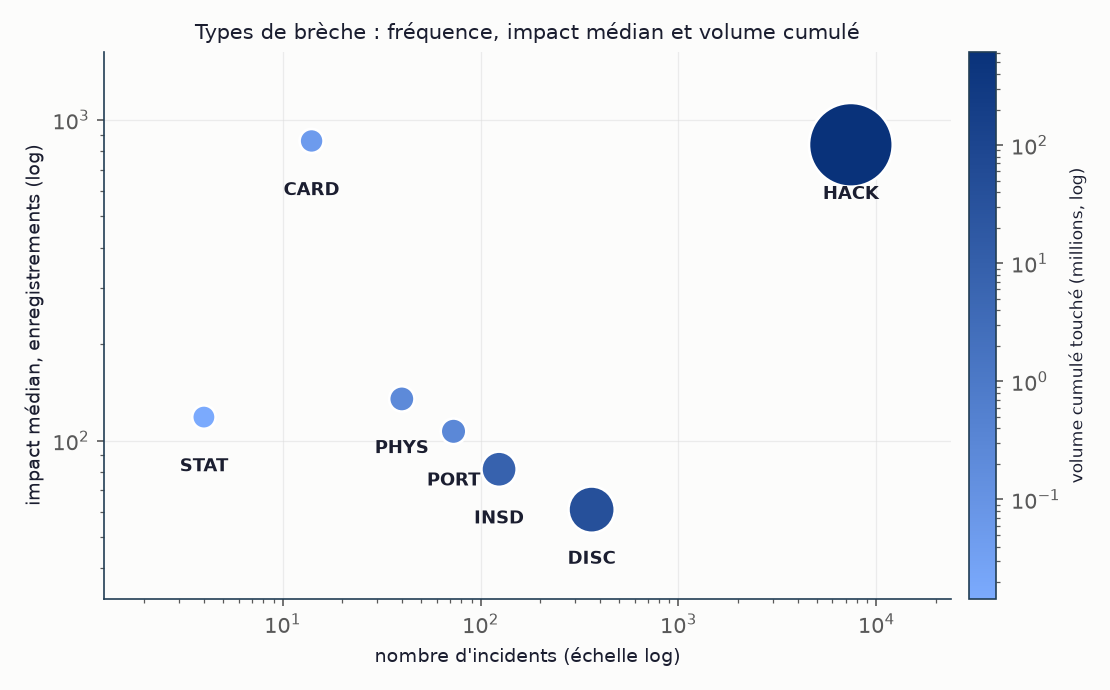
\includegraphics[width=0.90\textwidth]{../recherche/vasicek_lab/figures/D3_bulles_breche.png}
\caption{Types de brèche dans le plan fréquence contre impact médian, la taille et la teinte des
disques portant le volume cumulé. Les deux axes sont logarithmiques.}
\label{fig:bulles-breche}
\end{figure}

La figure~\ref{fig:bulles-breche} sépare ce que le seul comptage confond. Le piratage domine les
deux dimensions à la fois, avec $7\,430$ incidents et un impact médian de $836$ enregistrements,
ce qui en fait le seul type simultanément fréquent et lourd. La divulgation involontaire est le
deuxième en fréquence mais le plus léger en médiane, à $61$ enregistrements. À l'opposé, la
fraude à la carte ne compte que quatorze incidents pour une médiane de $860$, la plus haute de la
table : un type rare peut porter une sévérité unitaire élevée sans peser sur la charge, et
l'inverse est vrai.

\begin{cle}
\textbf{Ce que cette section change au modèle.} Trois mesures convergent vers la même
conclusion, obtenues par trois instruments indépendants : le $V$ de Cramér sous $0{,}20$, le
$\varepsilon^2$ sous $0{,}08$ et les corrélations de rang sous $0{,}16$. La catégorie d'un
incident et la taille de l'entité qui le subit informent faiblement sa sévérité. Segmenter la
queue sur l'une ou l'autre coûterait des degrés de liberté sans acheter de pouvoir explicatif.
Le mémoire ajuste donc une queue commune, et cette décision est ici une \emph{mesure} plutôt
qu'une commodité : elle est adossée à des tailles d'effet publiées, pas à une hypothèse de
simplicité.
\end{cle}

%--------------------------------------------------------------

% Origine : chapitres_sfe/03_donnees.tex, « Portée et limites du dispositif de données », deplace le 2026-10-01 (phase 4). Le corps en garde un resume.
\section{Portée et limites du dispositif de données}
% [etiquette sec:portee-donnees gardee dans le corps]

La discipline méthodologique retenue dans ce mémoire consiste à ne jamais
prétendre inférer davantage que ce que les données permettent réellement, ce
qui impose d'expliciter aussi bien les capacités que les limites du dispositif.

\paragraph{Ce que l'on sait faire.} On sait lire une fréquence d'incidents
matériels sur des pertes observées (OpRisk Global), et la moduler entre états de
conformité selon une structure d'attaque citée (Hackmageddon).
On sait calibrer une sévérité de queue lourde par la théorie des valeurs
extrêmes à partir de pertes réellement observées (OpRisk Global), et
confronter cette calibration à une source indépendante pour objectiver
l'incertitude. On sait enfin traiter l'écart entre sources non comme un bruit
à éliminer, mais comme une dimension d'incertitude à part entière, qui
s'ajoute à l'incertitude de paramètre estimée par bootstrap.

\paragraph{Ce que l'on ne sait pas faire.} On ne sait pas mesurer directement
le niveau de conformité DORA d'une entité donnée ; c'est précisément la
raison d'être de l'état de conformité par pilier introduit au
chapitre~\ref{chap:multietats}. On ne sait pas
disposer d'une base d'incidents harmonisée à l'échelle européenne, exhaustive
et non biaisée par la visibilité médiatique. On ne sait pas non plus estimer
avec précision la corrélation entre les différentes briques de perte,
faute d'historique suffisant sur les événements joints ; cette incertitude
est traitée au chapitre~\ref{chap:cascade} par une structure de dépendance explicite plutôt que
par une hypothèse d'indépendance non fondée.

Deux règles du moteur de simulation, le plafond de sévérité propre à la source PRC et la
sévérité nulle sous le seuil, ainsi que la suffisance des trois sources pour un exercice
d'ORSA, sont précisées \matcomp.

% SOURCES-SCRIPTS: 05 63

% Origine : chapitres_sfe/03_donnees.tex, « Le choix d'un nombre restreint de sources », deplace le 2026-10-01 (phase 4). Le corps en garde un resume.
\section{Le choix d'un nombre restreint de sources}

Des bases
supplémentaires existent (bases commerciales de sinistres cyber assurantiels,
enquêtes sectorielles européennes) et pourraient, en principe, enrichir le
dispositif. Mais chacune porterait ses propres biais de sélection et de
représentativité, sans lever la limite structurelle identifiée plus haut :
l'absence, à ce jour, d'un registre harmonisé et exhaustif à
l'échelle du marché. Multiplier les sources déplacerait la difficulté sans la
résoudre, et complexifierait un dispositif dont les rôles sont aujourd'hui distincts (trois
sources, trois rôles, aucune hiérarchie de \og source primaire\fg{}). L'analyse de sensibilité menée
au chapitre~\ref{chap:resultats} confirme d'ailleurs, \emph{a posteriori}, la pertinence de ce choix :
c'est l'incertitude sur l'indice de queue $\xi$ de la sévérité, estimé sur
les sources déjà mobilisées, qui domine très largement toute autre source
de variation du modèle, multipliers de fréquence et paramètres de dépendance
compris. Approfondir l'exploitation des trois sources retenues (bootstrap,
validation croisée, diagnostics de stabilité) réduit donc l'incertitude du
capital de façon bien plus significative que l'ajout d'une quatrième base de
sinistralité.

%--------------------------------------------------------------

%--------------------------------------------------------------

La structure tirée de Hackmageddon est confrontée au rapport \emph{ENISA Threat Landscape 2025}
\citep{enisa2025}, de méthodologie de collecte distincte, qui confirme la même hiérarchie des
vecteurs d'attaque par leur taux de conversion en intrusion \matcomp.

%==============================================================

\begin{cle}
\textbf{Ce que ces données permettent, et ce qu'elles interdisent.} Elles fixent la queue de
sévérité ($\hat\xi = 0{,}595$ sur OpRisk), la fréquence d'entrée et l'accumulation par cause
commune. Elles ne fixent \emph{pas} la direction de la contagion : le
chapitre~\ref{ch:identifiabilite} le montre sur trois sources qui échouent pour des raisons
distinctes, et le
chapitre~\ref{chap:partielle} en tire les conséquences en bornes de capital. Cette frontière
est un résultat produit par le dispositif de données, non une lacune de celui-ci.
\end{cle}

% =====================================================================

% SOURCES-SCRIPTS: 05 62 63

% Origine : chapitres_sfe/10_robustesse.tex, « Limites du domaine et limites de ce travail », deplace le 2026-10-01 (phase 4). Le corps en garde un resume.
\section{Limites du domaine et limites de ce travail}
% [etiquette sec:deux-natures-limites gardee dans le corps]

% SOURCES-SCRIPTS: 110

Les trois dernières lignes de la table, et le registre de la section~\ref{ch:livrable}, mêlent
deux natures de limites que rien ne distingue à la lecture. Les unes tiennent à ce qu'aucune
source disponible aujourd'hui ne permet de calibrer, à quiconque et non au seul présent travail.
Les autres tiennent à ce que ce travail a choisi de ne pas faire. Les confondre fait lire les
premières comme des insuffisances, alors qu'elles sont le fait qui commande la méthode.

\paragraph{Ce que la donnée cyber interdit aujourd'hui.} La direction de la contagion entre
domaines de contrôle n'est enregistrée par aucune source, et ce constat est mesuré plutôt
qu'affirmé : le schéma VERIS porte le champ qui l'identifierait, renseigné dans $0{,}12\,\%$ des
incidents de sa base publique, et la chronologie qui porterait l'antériorité dans $1{,}19\,\%$ ;
leur intersection compte un incident, aucun en secteur financier
(section~\ref{ch:livrable}). La non-identifiabilité n'est donc pas une propriété des sources
retenues ici, c'est une propriété du reporting d'incidents tel qu'il existe. Le coût d'un
sinistre touchant plusieurs piliers n'est davantage observé par aucune source, et la sévérité
d'une perte cyber en euros n'est disponible à cette profondeur que sur des bases de risque
opérationnel bancaire, ce qui fixe le périmètre de calibration du chapitre~\ref{chap:socle} et
la borne inférieure de validité du chapitre~\ref{chap:resultats}.

\paragraph{Ce que le mémoire en fait.} Devant une grandeur que la donnée ne détermine pas, deux
conduites sont possibles : en poser une valeur et la présenter comme une estimation, ou établir
la non-identifiabilité, énumérer l'ensemble admissible et publier des bornes. La seconde est
retenue partout, et elle s'accompagne d'une exigence : vérifier que la conclusion survit à
l'ensemble entier et non à un point choisi, ce que portent le lemme de monotonie en $g$ et
l'invariance de l'ordre de remédiation. Il en résulte une lecture qui vaut pour tout le
mémoire : l'\emph{amplitude} du surcoût est un scénario, son \emph{signe} et son \emph{ordre}
sont des résultats. Un paramètre posé n'est alors pas une faiblesse, c'est un périmètre déclaré.

\paragraph{Ce qui relève de ce travail.} Le reste du registre est d'une autre nature et
s'arbitre. L'élicitation structurée a été préparée et diffusée, et elle est restée sans réponse
(annexe~\ref{ch:elicitation}) ; la calibration est gelée, et les
corrections d'erreur seules y restent admises ; une source de structure est citée sans être
recalculable, sous un statut déclaré ; deux écarts d'estimation involontaires sont publiés avec
leur sens plutôt que corrigés. Ces décisions appartiennent à l'auteur et auraient pu être prises
autrement : c'est ce qui les sépare des précédentes. Une limite du domaine ne se corrige pas en
travaillant davantage sur ce mémoire, mais par le registre d'incidents spécifié à la
section~\ref{ch:livrable} ; une limite de ce travail se corrigerait en y revenant.

% Origine : chapitres_sfe/10_robustesse.tex, « Les trois étages de l'incertitude du SCR », deplace le 2026-10-01 (phase 4). Le corps en garde un resume.
\section{Les trois étages de l'incertitude du SCR}
% [etiquette sec:trois-etages gardee dans le corps]

L'incertitude sur le SCR ne se réduit pas au paramètre. Elle se répartit sur trois étages, qu'il
faut nommer plutôt que confondre (figure~\ref{fig:bande-modele}). Le premier est l'incertitude
de paramètre : l'intervalle de confiance de $\xi$ à lui seul dilate la VaR d'un facteur
$2{,}5$ sur la calibration figée, valeur que le bootstrap retrouve à la précision près.
% SOURCES-SCRIPTS: 63 46
Le deuxième est l'incertitude d'identification :
la direction de $W$ n'étant pas identifiable, la contagion se lit en bande
(chapitre~\ref{chap:partielle}). Le troisième, le plus souvent passé sous silence, est
l'incertitude de modèle : le choix de la \emph{famille} elle-même.

On la chiffre en recalculant le SCR sous des familles concurrentes. Sur l'axe de la
\emph{dépendance}, à marges par pilier fixées, le SCR va de $5\,322$ M\euro{} (indépendance) à
$9\,806$ M\euro{} (comonotone, borne de Fréchet), soit un facteur $1{,}8$, la formule standard
Solvabilité~II et les copules gaussienne et de Gumbel se plaçant entre les deux ; la cascade
dirigée ($8\,318$ M\euro) tombe dans cette bande, entre une dépendance gaussienne et une
dépendance de Gumbel. Sur l'axe de la famille de queue, l'écart est bien plus large :
d'une lognormale ($4\,330$ M\euro) à une GPD à queue lourde ($\xi=0{,}90$ ; $24\,016$ M\euro),
un facteur $5{,}5$. C'est le choix de la loi de queue qui domine, de loin, l'incertitude de
modèle, et c'est précisément pourquoi le plafond de réassurance ($40$ M\euro) est un levier
distinct, qui ramène la famille lourde à $495$ M\euro : une réponse au risque de queue, non le
risque lui-même.

\begin{figure}[htbp]\centering
\figover{J4_bande_modele.png}
\caption{La bande de modèle, troisième étage d'incertitude. (a)~axe dépendance, à
marges fixées : la cascade se place entre les copules gaussienne et de Gumbel, dans une bande
$[5{,}3\,;9{,}8]$ Md\euro. (b)~axe famille de queue : la queue lourde domine
l'incertitude ($\times 5{,}5$). (c)~les trois étages (paramètre, identification,
modèle) tels que le script les cumule ; la bande \emph{reportée} par le mémoire n'en retient que
les deux premiers, le troisième étant publié comme axe de sensibilité
(\S\ref{sec:etage-modele-hors-bande}).}
% SOURCES-SCRIPTS: 48
\label{fig:bande-modele}
\end{figure}

\subsection{Deux étages dans la bande reportée, le troisième hors bande}
% [etiquette sec:etage-modele-hors-bande gardee dans le corps]

Les trois étages ne peuvent pas tous entrer dans un intervalle unique. La bande reportée par ce mémoire ne cumule que les deux premiers,
paramètre et identification. L'étage de modèle est publié, mais comme axe de
sensibilité déclaré et non comme composante de la bande.

\paragraph{Les trois étages, mis sur une seule échelle avant toute comparaison.} Comparer les
étages exige de les lire sur la \emph{même} grandeur, première chose à faire ici :
l'étage de paramètre est publié sur le quantile d'\emph{un sinistre} (facteur $2{,}5$) tandis que
les deux autres vivent sur la \emph{charge annuelle agrégée}. Les rapprocher tels quels
comparerait deux échelles, ce qui est précisément l'erreur que ce mémoire s'interdit ailleurs.
Porté sur l'agrégat, l'intervalle bootstrap de $\xi$ donne $[3\,042\,;\,27\,152]$~M\euro, soit un
facteur $8{,}93$ : le quantile annuel amplifie l'incertitude de paramètre, et le facteur
$2{,}5$ ne mesure donc pas ce que le paramètre fait au \emph{capital}.
% SOURCES-SCRIPTS: 71

\begin{center}\footnotesize
\renewcommand{\arraystretch}{1.25}
\begin{tabular}{@{}l l r@{}}
\toprule
\textbf{Étage, lu sur la charge annuelle} & \textbf{Bande} & \textbf{Facteur} \\
\midrule
Paramètre ($\xi$ sur son IC$_{90}$) & $[3\,042\,;\,27\,152]$ & $8{,}93$ \\
Identification (direction de $W$) & $[6\,858\,;\,8\,697]$ & $1{,}27$ \\
Modèle, axe dépendance & $[5\,322\,;\,9\,806]$ & $1{,}84$ \\
Modèle, axe famille de queue & $[4\,330\,;\,39\,901]$ & $9{,}21$ \\
\bottomrule
\end{tabular}
\end{center}

\vspace{4pt}
\noindent En M\euro. La hiérarchie ainsi rétablie n'est pas celle qu'on annonce d'ordinaire :
\textbf{l'étage de modèle n'écrase pas les autres}, il est du même ordre que l'étage de paramètre,
et les deux dominent largement l'identification. Le retirer ne peut donc pas se justifier par sa
taille, et l'argument qui suit est d'une autre nature. Réserve à garder : ces largeurs de
paramètre font varier $\xi$ seul, $\sigma$ restant à sa valeur publiée, alors que le bootstrap
estime le couple conjointement ; ce sont donc des \emph{majorants}.

\paragraph{Pourquoi l'étage de modèle sort de la bande.} Les deux étages retenus sont
statistiques, portables par un intervalle ; le troisième est épistémique, un choix de famille ne
se moyennant pas. Sur l'axe de la famille de queue, il pousse l'indice de queue à une valeur
posée hors de l'intervalle bootstrap, et le cumuler mettrait un scénario et une borne de
confiance dans le même objet. Il reste publié deux fois, comme pire cas de modèle dans l'échelle
des postures et comme bande de dépendance ci-dessus, et l'ordre d'amorce des piliers ne bouge
pas \matcomp.

\paragraph{Sur l'auto-excitation : une équivalence observationnelle.} Une cascade sans aucune
auto-excitation, simulée puis ajustée comme une chronologie réelle, donne au jour un ratio de
branchement de $0{,}480$, à comparer au $0{,}551$ mesuré. Le processus de Hawkes n'est donc pas
distinguable de la cascade à la résolution disponible, et la cascade est retenue par parcimonie
interprétative, puisqu'elle porte en outre la structure entre piliers. Dégrader la résolution
fait monter le ratio estimé, et le préprint de cascade climatique converge sur ce choix sans le
tester. Le détail est déporté \matcomp.
% SOURCES-SCRIPTS: 85

\begin{cle}
\textbf{Oui, chaque brique a des alternatives.} Fréquence (Poisson, Hawkes, Cox), sévérité
(lognormale, splicing, EVT bayésienne), dépendance (copules, réseaux, Hawkes multivarié),
mesure (TVaR, spectrale, robuste), agrégation (formule standard, Panjer) : on ne prétend pas
détenir \emph{la} méthode. La discipline est ailleurs : on a testé les concurrents les plus
sérieux, on borne l'effet du choix, et surtout le niveau bouge dans la bande mais
l'ordre d'amorce des piliers ne bouge pas ($P1>P4>P2>P3>P5$, invariant à la famille).
Le niveau est illustratif, l'ordre résiste : c'est, chiffrée sur un troisième axe, la thèse du
mémoire, et la réponse à qui demanderait \og et si vous aviez pris une autre méthode~?\fg.
\end{cle}

% Origine : chapitres_sfe/10_robustesse.tex, « Contrôle du moteur d'agrégation par trois chemins indépendants », deplace le 2026-10-01 (phase 4). Le corps en garde un resume.
\section{Contrôle du moteur d'agrégation par trois chemins indépendants}
% [etiquette sec:triangulation-agregation gardee dans le corps]

Tout ce que les sections précédentes valident, elles le valident \emph{contre la donnée} :
adéquation, balayage de seuil, bootstrap, transformation intégrale de probabilité, test hors
échantillon. Aucun de ces contrôles ne regarde le moteur qui transforme une loi de fréquence et
une loi de sévérité en un quantile annuel. Un diagnostic de convergence de Monte-Carlo n'y
supplée pas : il établit que l'estimateur est \emph{stable}, jamais qu'il est \emph{juste}, et un
biais systématique de l'agrégation lui resterait invisible. La charge annuelle du modèle étant
exactement une somme composée, $S=X_1+\dots+X_K$ avec $X_i = u + \mathrm{GPD}(\xi,\sigma)$, elle
se calcule aussi sans simuler, ce que fait cette section.

Le nombre $K$ de pertes non nulles d'une année se construit en trois étages tous exacts : les
amorces suivent la binomiale négative, chaque amorce touche un ensemble de piliers dont les
tables de cascade énumèrent la loi, et chaque pilier touché ne produit une perte qu'avec la
probabilité de dépassement du seuil. Sa fonction génératrice s'écrit donc en forme fermée, ce qui
ouvre deux voies étrangères au Monte-Carlo. L'inversion par transformée de Fourier donne
la loi agrégée sans aucun aléa : c'est la réalisation numériquement stable de la récursion de
\citet{panjer1981} \citep{embrechtsfrei2009}, laquelle est inexploitable telle quelle à l'indice de
queue publié, où elle demanderait une grille de plusieurs millions de points parcourue de proche en
proche. L'\emph{approximation par perte unique} \citep{bockerkluppelberg2005} exploite la sous-exponentialité de la sévérité, sous laquelle la survie de la somme vaut
asymptotiquement $\mathbb{E}[K]$ fois celle d'une perte isolée : elle donne une forme fermée,
raffinée au second ordre par une correction de moyenne.

\begin{center}\footnotesize
\renewcommand{\arraystretch}{1.25}
\begin{tabular}{@{}l l r r@{}}
\toprule
\textbf{Méthode} & \textbf{Nature} & \textbf{Conforme} & \textbf{Non conforme} \\
\midrule
Monte-Carlo (moteur publié) & stochastique & $6\,049$ & $20\,188$ \\
Inversion par Fourier & numérique exacte & $5\,945$ & $19\,890$ \\
Perte unique, second ordre & analytique & $5\,448$ & $18\,632$ \\
Perte unique, premier ordre & analytique & $4\,989$ & $14\,933$ \\
\bottomrule
\end{tabular}
\end{center}

\vspace{4pt}
\noindent En M\euro, $\VaR$ à $99{,}5\,\%$ de la charge annuelle. Écarts à la référence
Monte-Carlo : $-1{,}7$ et $-1{,}5\,\%$ pour l'inversion, $-9{,}9$ et $-7{,}7\,\%$ au second ordre
analytique, $-17{,}5$ et $-26{,}0\,\%$ au premier.

\textbf{Lecture, et elle ne se fait pas contre zéro.} La référence est elle-même une grandeur
simulée : sa moyenne sur quatre graines porte une erreur type de $139$ et $500$~M\euro{} selon
l'état. L'écart de l'inversion vaut $0{,}75$ et $0{,}59$ erreur type, donc il n'est pas
résolu. Deux chemins qui ne partagent ni code ni aléa, l'un tirant des années et l'autre
composant des transformées, ne se séparent pas à la résolution disponible : c'est le meilleur
résultat que ce contrôle pouvait rendre ; c'est aussi la raison de ne pas citer le $-1{,}7\,\%$
seul, qui se lirait comme un désaccord. L'approximation analytique, qui n'utilise ni simulation
ni inversion, reste à moins de dix pour cent au second ordre contre plus du double au premier :
la correction de moyenne rattrape l'essentiel, comportement que la théorie annonce pour une
approximation asymptotique lue à un niveau fini.

Deux garde-fous numériques sont mesurés plutôt que supposés, parce qu'ils décideraient du
résultat. La transformée discrète étant circulaire, la masse qui dépasse la grille revient dans
les petits montants et gonfle le quantile : elle vaut ici $1{,}65\cdot 10^{-8}$, soit quatre ordres
de grandeur sous le niveau de dépassement. Et la sévérité est discrétisée par les masses et non
par la densité, ce qui laisse un écart de $0{,}063\,\%$ sur sa moyenne.

\begin{cle}
\textbf{Ce que ce contrôle établit, et ce qu'il n'établit pas.} Les quatre chemins partagent la
loi de fréquence, la loi de sévérité et les tables de cascade : ils contrôlent
l'\emph{agrégation}, jamais la vérité du modèle. C'est un contrôle d'instrument, du même genre
que celui qui impose au test de l'additivité des coûts de redonner les deux capitaux publiés à
exposant neutre, et il ne remplace aucun test contre la donnée. Sa portée est précise : le
quantile publié n'est pas un artefact du moteur de simulation.
\end{cle}

% SOURCES-SCRIPTS: 96

% Origine : chapitres_sfe/10_robustesse.tex, « VaR prédictive et VaR robuste », deplace le 2026-10-01 (phase 4). Le corps en garde un resume.
\section{VaR prédictive et VaR robuste}
% [etiquette sec:predictive-robuste gardee dans le corps]

Quantifier l'incertitude (les trois étages) ne dit pas encore \emph{quel} nombre reporter.
Prendre le quantile $99{,}5\,\%$ d'une loi estimée en un point (\emph{plug-in}) est fragile,
car les données sont incertaines : \og{}le quantile d'un objet incertain est mauvais\fg{}
(C.~Hillairet). Deux réponses complémentaires, selon la posture (figure~\ref{fig:robuste}),
le détail étant déporté \matcomp.

\textbf{La VaR prédictive} intègre l'incertitude de paramètre \emph{avant} de prendre le
quantile : on prend le quantile de la loi \emph{prédictive}, mélange des GPD sur la distribution
bootstrap de $(\xi,\sigma)$. Le résultat est instructif : à $99{,}5\,\%$ elle est \emph{quasi
égale} au \emph{plug-in} ($645$ contre $657$~M\euro, pour un bruit de simulation de $7$~M\euro,
donc un écart qui n'excède pas deux fois ce bruit) : le risque d'estimation n'est pas un
biais de point à ce niveau, il ne le devient qu'en profondeur ($+4\,\%$ à $99{,}9\,\%$). La
fragilité est dans la largeur de la bande, pas dans le point.

\textbf{La VaR robuste} prend au contraire la borne haute de la VaR sur l'ensemble
d'ambiguïté (paramètre, puis modèle) : la VaR robuste à $95\,\%$ vaut $1\,037$~M\euro{}
($1{,}6\times$ le \emph{plug-in}), le pire-cas de famille lourde $1\,331$~M\euro. C'est la
posture prudente, où le niveau de robustesse est un choix prudentiel explicite.

\paragraph{Les six postures, et ce que chacune intègre.} La figure~\ref{fig:robuste} en affiche
six, et les nommer ne suffit pas : une échelle dont les crans ne sont pas définis n'est pas une
échelle, c'est une suite de nombres. La table les définit donc une fois, avec la précision que
chacune supporte.

\begin{center}\footnotesize
\renewcommand{\arraystretch}{1.25}
\begin{tabular}{@{}l p{6.6cm} r r@{}}
\toprule
\textbf{Posture} & \textbf{Ce qu'elle intègre} & \textbf{VaR} & \textbf{bruit} \\
\midrule
Point (\emph{plug-in}) & rien : le quantile d'un ajustement ponctuel $(\hat\xi,\hat\sigma)$ & $657$ & --- \\
Prédictive & l'incertitude de paramètre, \emph{avant} le quantile, par mélange sur le bootstrap & $645$ & $\pm\,7$ \\
Robuste $\beta=90\,\%$ & la borne haute de la VaR sur l'ambiguïté de \emph{paramètre} : le quantile $\beta$ de la loi bootstrap de la VaR & $939$ & $\pm\,13$ \\
Robuste $\beta=95\,\%$ & idem, à un niveau de prudence plus élevé & $1\,037$ & $\pm\,9$ \\
Robuste $\beta=99\,\%$ & idem, la plus bruitée des six & $1\,247$ & $\pm\,24$ \\
Pire-cas de modèle & on ajoute l'ambiguïté de \emph{famille}, en poussant la queue à $\xi=0{,}90$ & $1\,331$ & --- \\
\bottomrule
\end{tabular}
\end{center}

\vspace{4pt}
\noindent En M\euro. Le bruit est l'écart-type de simulation sur quatre rééchantillonnages
indépendants, à $3\,000$ tirages bootstrap chacun. Deux lectures s'imposent, et la seconde
n'était pas attendue.

Les deux extrémités de l'échelle sont exactes et tout le bruit est au milieu ; la posture la
plus prudente est la moins précise. Les deux valeurs de la VaR prédictive, $648$ et $645$~M\euro,
sont un seul nombre à la précision du bruit. Le détail est déporté \matcomp.
% SOURCES-SCRIPTS: 46

\paragraph{Quelle posture le mémoire reporte-t-il.} La question mérite une réponse explicite,
puisque six valeurs vont de $657$ à $1\,331$~M\euro. Tous les capitaux publiés dans ce mémoire
sont bâtis sur la calibration figée, donc sur le \emph{plug-in}, et ils sont cités avec
leur bande d'identification partielle. L'échelle des postures n'est pas une alternative à ce
choix : c'est l'axe de sensibilité qui en donne le coût, et le passage du point au robuste
$95\,\%$ multiplierait le capital par $1{,}6$. Le choix d'une posture reportée relève de la
politique prudentielle de l'entité, non du modèle : le mémoire en retient une pour ses propres
chiffres, avec ses motifs (\S\ref{sec:posture-retenue}), et fournit la grille qui permet à une
entité d'en retenir une autre.

\begin{figure}[htbp]\centering
\figover{J7_scr_robuste.png}
\caption{VaR robuste. (a)~la VaR est elle-même incertaine ; le robuste en prend la
borne haute. (b)~l'échelle des postures, du point ($657$) au pire-cas de modèle
($1\,331$~M\euro), chacune avec son écart-type de simulation. Les deux extrémités n'en
portent aucun, étant déterministes ; la barre la plus longue est celle de $\beta=99\,\%$, la
posture la plus prudente et la moins précise.}
% SOURCES-SCRIPTS: 51
\label{fig:robuste}
\end{figure}

\begin{cle}
\textbf{Deux points qui intègrent l'incertitude.} La VaR prédictive est le point
\emph{central} (il embarque l'incertitude d'estimation) ; la VaR robuste est le point
\emph{prudent} (la borne haute sur l'ambiguïté). Le choix entre les deux relève de la politique
prudentielle, non du calcul. L'essentiel est de ne jamais reporter le seul \emph{plug-in} : le
SCR se cite avec sa bande, ou par un point qui assume l'incertitude, jamais nu.
\end{cle}

\subsection*{La posture retenue et ses motifs}
% [etiquette sec:posture-retenue gardee dans le corps]

% SOURCES-SCRIPTS: 46 51 63

\paragraph{Un fait qui rend le choix moins tranché qu'il n'y paraît : la robuste à
$\beta=95\,\%$ \emph{est} la borne haute de l'intervalle déjà publié.} La robuste au niveau
$\beta$ est le quantile $\beta$ de la loi bootstrap de la VaR ; l'intervalle publié à $90\,\%$ est
délimité par les quantiles $5$ et $95$ de cette même loi. Les deux valent donc $1\,037$~M\euro{},
et ce n'est pas une coïncidence numérique mais la même quantité sous deux noms. Reporter le
\emph{plug-in} avec sa bande publie donc déjà le chiffre robuste, comme une \emph{borne} et non
comme un point. Le désaccord entre les deux postures ne porte pas sur l'information mise à
disposition du lecteur, il porte sur ce qu'on appelle \og le \fg{} capital. La question se tranche
pour cela par la définition réglementaire plutôt que par la prudence.

Le paragraphe qui précède donne la grille ; il faut maintenant trancher, sans quoi le mémoire
laisserait son résultat central sans convention de report. La posture retenue est le
\emph{plug-in} accompagné de sa bande, la robuste restant publiée comme axe prudentiel déclaré.
Trois raisons convergent, et elles ne sont pas de même nature.

\textbf{La première est réglementaire, et elle vient en premier.} Le régime applicable définit le
capital de solvabilité requis comme une valeur en risque à $99{,}5\,\%$ de la variation des fonds
propres à un an. Une borne haute prise sur un ensemble d'ambiguïté n'est pas un quantile de la loi
de perte : c'est un supremum sur une famille de lois. La substituer répondrait à une autre question
que celle posée. Le risque d'estimation se traite dans le régime par la validation du modèle et par
le récit de l'ORSA, non en gonflant le quantile, et pour une raison de cohérence d'ensemble :
appliquée à chaque module, la même logique empilerait des marges dont le niveau de confiance global
ne serait plus énonçable.

\textbf{La deuxième est une mesure, celle qui rend le choix confortable.} La prédictive,
qui est la réponse théoriquement préférable puisqu'elle intègre l'incertitude \emph{avant} le
quantile, vaut $645$~M\euro{} contre $657$ pour le \emph{plug-in}, soit un écart de deux fois le
bruit de simulation. La bonne réponse ne déplace donc pas le point. Reporter la
prédictive remplacerait un nombre publié partout par un nombre indiscernable, au prix de la piste
d'audit et contre le gel de la calibration : le gain serait nul et le coût réel. Cette
coïncidence n'est pas générale et cesse en profondeur, l'écart passant à $+4\,\%$ à
$99{,}9\,\%$ : c'est en profondeur de queue, non au niveau réglementaire, que le choix de posture
commencerait à compter.

\textbf{La troisième est une question de précision, et elle va contre l'intuition.} Les postures
robustes sont les moins reproductibles des six, avec des écarts-types de simulation de $13$, $9$
et $24$~M\euro{} quand les deux extrémités de l'échelle n'en portent aucun. Reporter comme chiffre
de tête la valeur la moins précise contredirait la convention que ce mémoire s'impose par ailleurs,
à savoir que toute grandeur simulée se publie avec son bruit.

\begin{attention}
\textbf{Ce que cette décision ne dit pas.} La robuste n'est pas écartée : elle reste publiée, et
elle est le bon nombre pour un \emph{autre} usage. Dimensionner une couverture ou fixer une limite
de rétention est une décision sous ambiguïté, où l'on veut précisément la borne haute et non le
quantile central ; le \S\ref{sec:detenir-transferer} en est l'exemple. Une même grandeur peut donc
être reportée sous une convention et utilisée sous une autre, à condition de dire laquelle et
pourquoi, ce qui est fait ici.

\textbf{Et ce qui ferait rouvrir la décision}, énoncé d'avance pour qu'elle ne dépende pas d'une
préférence : un écart prédictive contre \emph{plug-in} qui dépasserait durablement quelques unités
de bruit au niveau réglementaire, ou un déplacement de l'objet du travail, du capital
\emph{reporté} vers une décision sous ambiguïté. Aucun des deux n'est le cas aujourd'hui.
\end{attention}

% Origine : chapitres_sfe/10_robustesse.tex, « Un défaut de calibration chiffré », deplace le 2026-10-01 (phase 4). Le corps en garde un resume.
\section{Un défaut de calibration chiffré}
% [etiquette sec:pu-coherence gardee dans le corps]

Un inventaire qui ne porterait que les hypothèses choisies serait incomplet : il doit aussi
porter les défauts connus. Il en reste un, de nature différente des précédents, car ce n'est
pas une hypothèse discutable mais une incohérence arithmétique.

La formule des dépassements de seuil prend trois entrées, le seuil $u$, le taux de dépassement
$p_u$ et le couple $(\xi,\sigma)$, pour deux degrés de liberté seulement : le seuil et
l'échantillon une fois fixés, $p_u$ se \emph{compte}, il ne se choisit pas. Or la calibration
figée publie $u=20{,}03$~M\euro{} et $p_u=0{,}1509$, quand ce seuil laisse $91$ excès sur $582$
pertes, soit $0{,}1564$. Le $0{,}1509$ vaut $88/583$, le taux du percentile $85$ d'un filtrage
antérieur resté dans la configuration après que le seuil eut bougé. Aucun état du monde ne rend
les deux valeurs vraies ensemble, et un lecteur qui pose la division le voit en trente secondes.

L'effet se chiffre exactement. Au taux cohérent, le quantile de sévérité à $99{,}5\,\%$ passerait
de $662{,}78$ à $678{,}60$~M\euro, soit $+2{,}4\,\%$, ou $15{,}8$~M\euro. Deux lectures de ce signe
doivent être distinguées, parce qu'on les confond volontiers. Du côté de la solvabilité, l'écart
est anti-conservateur : il sous-estime le besoin de capital, et une sous-estimation ne s'excuse
pas par la prudence, elle se déclare. Du côté de la thèse, il va dans l'autre sens, puisque le
chiffre avancé n'est pas gonflé par ce défaut mais minoré. Les deux sont vrais, ils ne portent
pas sur la même chose, et seul le premier engage.

La valeur est néanmoins gelée et l'écart inscrit au registre des limites : rejouer le pipeline
déplacerait des centaines de nombres publiés sans qu'aucun déplacement soit attribuable à la
correction \matcomp.

\paragraph{Le sens des écarts, en deux colonnes.} Un défaut isolé se pardonne ; une série de
défauts qui vont tous du même côté est un biais. Il vaut donc mieux mettre les deux colonnes
en regard une fois pour toutes, plutôt que de laisser le lecteur les rassembler lui-même.

\begin{center}\footnotesize
\renewcommand{\arraystretch}{1.3}
\begin{tabular}{@{}p{5.6cm} p{2.9cm} p{5.6cm}@{}}
\toprule
\textbf{Écart} & \textbf{Sens} & \textbf{Taille} \\
\midrule
\multicolumn{3}{@{}l}{\emph{Défauts d'estimation, tous trois anti-conservateurs}} \\
Taux de dépassement gelé ($p_u$) & sous-estime & $+2{,}4\,\%$ de VaR manquante \\
Couverture réelle de l'IC$_{90}$ de $\xi$ & sous-estime & $86\,\%$ au lieu de $90\,\%$ ; demi-largeur à élargir d'environ $10\,\%$ \\
Échelle de sévérité non stationnaire & sous-estime & dérive de $4{,}00\,\%$ par an dans la queue ($p=0{,}0386$), dont la moitié d'inflation monétaire ; au moins $+24{,}7\,\%$ sur le quantile, borne basse (\S\ref{soc:sec:backtest}) \\
\midrule
\multicolumn{3}{@{}l}{\emph{Choix posés, tous deux prudents}} \\
Charge systémique $a$ & majore & $0{,}60$ posé, au-delà de la borne haute empirique $0{,}22$ \\
Sur-dispersion du moteur $\varphi$ & majore & $9{,}20$ posé contre $2{,}24$ mesuré \\
\midrule
\multicolumn{3}{@{}l}{\emph{Limites de périmètre et de transposition, de sens opposés}} \\
Attritionnel absent de la donnée & sous-estime & non chiffrable : la base est tronquée à son seuil de collecte, les petits sinistres n'y figurent pas \\
Sévérité non plafonnée à l'échelle d'entité & majore & élasticité sévérité/taille $0{,}087$ $[0{,}026\,;0{,}148]$, presque nulle ; affecte le \emph{niveau} d'entité, et peut modifier les écarts entre états \\
\midrule
\multicolumn{3}{@{}l}{\emph{Hypothèse dont le sens n'est pas déterminable}} \\
Additivité des coûts au sein d'un sinistre multi-piliers & \textbf{indéterminé} & élasticité de l'écart $1{,}20$ ; $[9\,706\,;20\,487]$~M\euro{} pour $\theta\in[0{,}70\,;1{,}30]$, soit $76\,\%$ de l'écart publié (\S\ref{sec:additivite-couts}) \\
\bottomrule
\end{tabular}
\end{center}

\vspace{4pt}
\noindent La lecture est nette sur les cinq premières lignes. Les trois écarts
\emph{involontaires} d'estimation sous-estiment tous le capital ; les deux choix
\emph{délibérés} le majorent. La prudence du capital publié vient donc de choix déclarés, non de ses écarts d'estimation.
L'indice de queue n'est
pas de ces choix : le chiffre de tête repose sur la valeur estimée, et la valeur posée
plus lourde n'intervient que comme pire cas de modèle dans l'échelle des postures
(\S\ref{sec:predictive-robuste}), hors du capital reporté.

\vspace{2pt}
\noindent La troisième ligne pèse un quart quand les deux premières pèsent quelques
pour cent. Son effet sur l'écart entre états est mesuré, $-1{,}9\,\%$ et non résolu, et la moitié
de la dérive de queue est monétaire. Les deux lignes de périmètre bornent le niveau en sens
contraire : l'attritionnel absent de la donnée pèse peu au quantile d'entité, et le plafond de
sévérité qui amputerait le besoin de moitié ne va que de $53$ à $74$~M\euro{} sur des entités
dont la taille varie d'un facteur $134$. La dernière ligne, l'additivité des coûts, est la seule
dont le sens ne se déclare pas (\S\ref{sec:additivite-couts}). Le motif du gel, la lecture de
chaque ligne et le plafond chiffré sont déportés \matcomp.

\vspace{2pt}
% SOURCES-SCRIPTS: 08b 47 57 60 63 65 74 78 89 90 91

% Origine : chapitres_sfe/10_robustesse.tex, « Défaillances simultanées et additivité des coûts », deplace le 2026-10-01 (phase 4). Le corps en garde un resume.
\section{Défaillances simultanées et additivité des coûts}
% [etiquette sec:additivite-couts gardee dans le corps]

La cascade produit, pour chaque sinistre, un \emph{ensemble} de piliers touchés, si bien que la
défaillance simultanée n'est pas un cas particulier resté de côté mais la sortie même du modèle. La
loi exacte de ce nombre est donnée \matcomp : à l'état non conforme, la
défaillance multiple est majoritaire, $62{,}31\,\%$ des sinistres touchant plus d'un
pilier contre $31{,}15\,\%$ à l'état conforme. Reste la question de l'agrégation
des coûts, et elle demande de distinguer trois énoncés que le seul mot d'additivité recouvre.

\begin{enumerate}[leftmargin=*,itemsep=2pt]
\item \textbf{Au sein d'un sinistre}, les coûts des piliers touchés \emph{s'additionnent} : c'est
une hypothèse de construction, non testée, seul des trois que la question met en cause.
\item \textbf{En fonction des piliers non conformes}, le capital est \emph{presque additif},
$R^2=0{,}9945$ sur les $32$ configurations : c'est une mesure, et elle explique qu'une structure de
dépendance entre états ne déplace pas le capital espéré \matcomp.
\item \textbf{En fonction des quatre canaux}, il est \emph{franchement super-additif} en euros,
$+5\,001$~M\euro{} d'interaction sur $14\,139$, soit $+35\,\%$ (chapitre~\ref{chap:resultats}) :
c'est également une mesure, et elle traduit une composition quasi \emph{multiplicative} des
canaux, le logarithme du capital étant, lui, presque additif (\S\ref{sec:inverse}).
\end{enumerate}

\noindent Répondre \og~le modèle est super-additif~\fg{} serait donc faux : il l'est sur les canaux
et en euros, parce que leurs effets se multiplient, pas sur les piliers, et l'hypothèse sur les
coûts d'un incident est un troisième objet.

\paragraph{Sensibilité à l'additivité des coûts.} On fait varier cette hypothèse par un exposant, la
perte d'un sinistre touchant $k$ piliers valant $\bigl(\sum_j X_j\bigr)k^{\,\theta-1}$, de sorte que
$\theta=1$ redonne exactement le modèle publié et que les sinistres mono-pilier restent intouchés.
Pour $\theta$ parcourant $[0{,}70\,;1{,}30]$, l'écart entre états parcourt
$[9\,706\,;20\,487]$~M\euro, soit $76\,\%$ de l'écart publié et $15$~fois l'écart-type de
$734$~M\euro{} entre quatre graines. Cette sensibilité dépasse le bruit de simulation et fait de l'additivité des coûts
l'hypothèse structurelle non testée la plus influente sur l'\emph{écart}.

La queue de sévérité domine,
elle, l'incertitude sur le \emph{niveau} (\S\ref{sec:trois-etages}). L'additivité est une hypothèse de structure et non un choix
de prudence, les trois choix posés du \S\ref{sec:pu-coherence} déplaçant davantage mais dans une
direction connue.

\paragraph{Elle n'est pas neutre entre les deux états, ce qui n'était pas attendu.} Les élasticités
valent $0{,}95$ à l'état non conforme contre $0{,}39$ à l'état conforme, un facteur $2{,}42$, parce
que l'exposant ne mord que sur les sinistres multi-piliers, majoritaires au seul état non conforme.
L'hypothèse interagit donc avec le canal de propagation au lieu de s'ajouter à côté de lui,
et atteint de ce fait la grandeur centrale du mémoire et non un simple niveau. Ce qui tient malgré
tout : sur toute l'amplitude examinée l'écart garde son signe et son ordre de grandeur, jamais
proche de zéro, si bien que la thèse ne dépend pas de l'hypothèse d'additivité et que seule son
amplitude en dépend. C'est la structure d'argument déjà employée pour les valeurs de $g$.

Le \emph{sens} de la non-additivité, lui, n'est pas déterminable : mutualisation de la remédiation
et saturation de la capacité de réponse tirent en sens contraire, et aucune source ne les sépare. Le
détail, la loi du nombre de piliers, la table complète des exposants et la raison pour laquelle
l'amplitude est posée plutôt qu'estimée sont déportés \matcomp.

\paragraph{Croisée avec le plafond de sévérité, elle s'efface là où il mord.} La limite de
périmètre du \S\ref{sec:pu-coherence} tire en sens inverse : un plafond de sévérité adossé à
l'exposition $E$ de l'entité, à une fraction $\kappa$ de celle-ci, abaisserait le besoin quand un
exposant $\theta > 1$ le relève. Les deux réserves sont mesurées ensemble sur l'entité notionnelle,
la perte d'un sinistre valant $\min\bigl(\kappa E,\,(\sum_j X_j)\,k^{\,\theta-1}\bigr)$
(figure~\ref{fig:plafond-saturation-corps}). Elles ne se compensent pas : le terme d'interaction est
positif sous $\theta = 1$ et négatif au-delà, le plafond atténuant la saturation dans les deux sens,
jusqu'à l'effacer à $\kappa = 0{,}5\,\%$, où le besoin vaut $96{,}2$~M\euro{} pour les cinq
exposants. Aucun couple où le plafond mord ne ramène le besoin à sa valeur libre, $179{,}1$~M\euro{}
dans ce moteur simulé au niveau du sinistre, du même ordre que les $169$ publiés. Les deux réserves sont donc hiérarchisées et non confondues, et la bande
conjointe, $177{,}8$~M\euro{}, reste sous la somme des deux bandes marginales, $203{,}7$ : les
additionner surestimerait l'incertitude.

\begin{figure}[H]\centering
\figover{S34_plafond_saturation_3d.png}
\caption{La saturation et le plafond croisés sur l'entité notionnelle. (a)~le besoin de capital,
avec la ligne plate à $\kappa = 0{,}5\,\%$ où la sensibilité à $\theta$ est nulle. (b)~le terme
d'interaction, nul à $\theta = 1$, positif en deçà et négatif au-delà : le plafond est un
amortisseur et non un contrepoids. L'axe des plafonds est ordinal, son dernier cran étant l'absence
de plafond.}
\label{fig:plafond-saturation-corps}
\end{figure}

\vspace{2pt}
% SOURCES-SCRIPTS: 74 68 69 86 109


\begin{cle}
\textbf{La double lecture.} \og Insensible aux choix innocents, sensible aux leviers réels \fg :
le modèle n'est ni sur-ajusté ni fragile, il est piloté par ce qui doit le piloter.
Et la seule grande incertitude, la queue, est nommée et bornée, pas cachée. C'est ce qui
sépare un modèle dont tout n'est pas calibré d'un modèle dont on ignore de quoi il dépend :
ici, la dépendance du capital est établie levier par levier, et son absence aussi.
\end{cle}

% =====================================================================

% Origine : chapitres_sfe/10_robustesse.tex, « Recommandations sur la donnée manquante », deplace le 2026-10-01 (phase 4). Le corps en garde un resume.
\section{Recommandations sur la donnée manquante}
% [etiquette ch:livrable gardee dans le corps]

\begin{cle}
\textbf{Idée directrice.} Le chapitre~\ref{ch:identifiabilite} a montré que la direction de la
contagion n'est pas identifiable sur les sources agrégées. Cette limite n'est pas un point final :
elle se retourne en spécification de reporting, et cette spécification se chiffre
puis se hiérarchise. C'est la contribution réglementaire du travail, et elle ne dépend
d'aucun prior.
\end{cle}

\subsection{Contenu d'un registre d'incidents}

Puisque les trois sources agrégées échouent pour des raisons \emph{distinctes} (la première
manque de taxonomie et de volume informatif, la deuxième de résolution temporelle, la troisième
possède les bons champs mais ne les renseigne pas), la donnée qui identifierait $W$ se déduit
par complémentarité, et la proposition~\ref{prop:nonid} y ajoute une exigence. Un registre
d'incidents TIC l'identifiant devrait :
\begin{enumerate}[itemsep=2pt]
\item horodater la survenance (et non la seule déclaration) au mois ou à la
      semaine, afin de porter une antériorité que le pas annuel efface ;
\item catégoriser par domaine de contrôle (les piliers DORA), et non par vecteur
      d'attaque, afin qu'une transition soit interprétable comme un lien $k \to j$ ;
\item consolider une cause commune comme \emph{un} événement à $N$ victimes, pour ne pas
      confondre un lot de déclaration avec une contagion séquentielle ;
\item consigner, pour chaque incident, l'ensemble des piliers qui ont cédé, y compris ceux qui
      n'ont rien entraîné. Même sans horodatage, la loi jointe des piliers touchés distingue une
      matrice de sa transposée : sur la matrice publiée, la part des sinistres touchant plus d'un
      pilier vaut $62{,}31\,\%$ sous $W$ et $50{,}77\,\%$ sous $W^\top$.
\end{enumerate}

Ces exigences ne sont pas hors d'atteinte, mais elles ne relèvent pas du même instrument. Le
registre d'information du règlement d'exécution \citep{eu2024_2956} porte sur les accords
contractuels avec les prestataires : il identifie les prestataires, la chaîne de sous-traitance et
la criticité des fonctions, ce qui sert la troisième exigence en permettant de rattacher des
incidents à un même prestataire. Les trois autres relèvent de la notification des incidents
majeurs, dont il s'agit de fixer le \emph{format} de l'horodatage et le \emph{choix de la
taxonomie} plutôt que d'organiser une collecte nouvelle.

\begin{cle}
\textbf{La spécification n'est même pas à écrire : elle existe et n'est pas remplie.} Les deux
premières exigences ci-dessus sont déjà des champs du schéma VERIS, standard ouvert de
description d'incidents et support du \emph{Data Breach Investigations Report} : le champ
\texttt{control\_failure} porte le domaine de contrôle défaillant, et une chronologie en quatre
étapes (compromission, exfiltration, découverte, confinement) porte l'antériorité. Sur les
$10\,591$ incidents de la base publique associée, le premier est renseigné dans $0{,}12\,\%$ des
cas et la seconde, sur au moins deux étapes, dans $1{,}19\,\%$ ; leur intersection ne
compte qu'un seul incident, et aucun en secteur financier
(chapitre~\ref{ch:identifiabilite}). La recommandation change alors de nature. Elle ne demande
pas d'inventer une taxonomie, ce qui serait long et contestable, mais de rendre
obligatoires deux champs déjà normalisés dans un dispositif, la notification
d'incident majeur sous DORA, qui a précisément le pouvoir de l'imposer là où une base
déclarative volontaire ne l'a pas. C'est un coût de conception nul et un gain d'identification
chiffré à la section suivante.
\end{cle}

% SOURCES-SCRIPTS: 28 52 08b 98 110

% SOURCES-SCRIPTS: 52 08b


\subsection{Valeur en capital de l'information}

Une recommandation de reporting reste un v\oe u tant qu'elle n'est pas chiffrée. On la chiffre en
restreignant l'ensemble admissible du chapitre~\ref{chap:partielle} aux configurations compatibles
avec l'information acquise, puis en mesurant le rétrécissement de la bande de capital.

\begin{definition}[Valeur d'information d'une contrainte]% [etiquette def:voi gardee dans le corps]
Soit $\mathcal{W}$ l'ensemble admissible et $\mathrm{SCR}:\mathcal{W}\to\R_+$ la fonctionnelle de
capital. La largeur de bande associée à un sous-ensemble $\mathcal{V}\subseteq\mathcal{W}$ est
\begin{equation}
  L(\mathcal{V}) \;=\; \sup_{W\in\mathcal{V}}\mathrm{SCR}(W)\;-\;\inf_{W\in\mathcal{V}}\mathrm{SCR}(W).
  % [etiquette eq:largeur-bande gardee dans le corps]
\end{equation}
Une information $\mathcal{I}$ qui restreint l'ensemble à $\mathcal{W}_{\mathcal{I}}\subseteq
\mathcal{W}$ a pour valeur le rétrécissement relatif qu'elle produit :
\begin{equation}
  V(\mathcal{I}) \;=\; 1-\frac{L(\mathcal{W}_{\mathcal{I}})}{L(\mathcal{W})} \;\in\;[0,1].
  % [etiquette eq:voi gardee dans le corps]
\end{equation}
\end{definition}

Cette définition a deux propriétés utiles. Elle est monotone : si
$\mathcal{I}'$ implique $\mathcal{I}$, alors $\mathcal{W}_{\mathcal{I}'}\subseteq
\mathcal{W}_{\mathcal{I}}$ et donc $V(\mathcal{I}')\ge V(\mathcal{I})$, une information plus
riche ne pouvant pas valoir moins. Et elle est sans dimension, donc indépendante du
niveau de capital, ce qui la rend comparable d'une source de sévérité à l'autre alors même que
ce niveau, lui, varie d'un facteur quarante.

Les sept premiers rapports post-incident du corpus du chapitre~\ref{ch:identifiabilite} documentent le
\emph{sens} de six des dix dépendances entre piliers, sens que le \S\ref{sec:bayes} ne revendique
paire par paire que sur deux d'entre elles. Retenu sur les six, il ferait tomber la largeur de la
bande de $66\,\%$. Ce chiffre est donc la valeur, en capital, d'une information de sens de cette
étendue, non un acquis du mémoire, et il donne l'ordre de grandeur de ce qu'un registre
correctement spécifié apporterait.

\begin{attention}
\textbf{Ce qu'aucune information de sens ne donnera.} Même les dix directions établies, une bande
subsisterait, imputable à la seule amplitude des coefficients : connaître le sens d'un
lien ne donne pas sa force. L'identification partielle n'est donc pas un état provisoire que la
donnée finirait par lever, elle est structurelle. C'est une raison de plus de lire le
capital en bande, et de ne pas promettre à un superviseur davantage que ce qu'un registre peut
tenir.
\end{attention}

% SOURCES-SCRIPTS: 66 55


\subsection{Priorités de documentation des dépendances}

L'apport le plus actionnable est ailleurs que dans le total. En fixant le sens d'\emph{une seule}
dépendance à la fois, on obtient un classement des données manquantes par valeur
d'information (figure~\ref{fig:voi}). Le classement est très inégal : documenter la seule dépendance
entre gouvernance et gestion des incidents lèverait $28{,}9\,\%$ de
l'ambiguïté de capital, tandis que documenter le lien entre tests et tiers n'en lèverait
\emph{rien}.

% [H] APRES LE PARAGRAPHE QUI L'APPELLE (phase 3) : en [htbp] sous le titre, la figure se posait
% en tete de page au milieu de la phrase « gouvernance et | gestion des incidents ».
% [environnement fig:voi garde dans le corps du rapport]

Deux conséquences pratiques. D'abord, un superviseur qui ne pourrait exiger qu'une seule
dépendance sait désormais laquelle demander, et une entité qui ne pourrait instrumenter qu'un seul
lien sait lequel instrumenter. Ensuite, un fait qui oriente la recommandation : la
dépendance la plus précieuse est précisément celle que le corpus documentaire ne couvre pas. La
lecture de rapports publics a livré ce qu'elle pouvait livrer ; le reste exige la donnée d'entité.

% SOURCES-SCRIPTS: 55

\begin{cle}
\textbf{La limite devenue contribution.} Un mémoire qui se contenterait de constater qu'il ne
peut pas calibrer $W$ laisserait le lecteur sans suite. En spécifiant la donnée qui manque, en
chiffrant ce qu'elle vaut et en la hiérarchisant, on transforme une frontière d'identification en
\emph{recommandation opposable}, adressée au cadre de reporting que DORA met précisément en
place. C'est le seul endroit du mémoire où une limite produit un livrable.
\end{cle}

% =====================================================================

% Origine : chapitres_sfe/09_resultats.tex, « SCR par état de conformité », deplace le 2026-10-01 (phase 4). Le corps en garde un resume.
\section{SCR par état de conformité}

Le SCR croît de façon monotone de l'état conforme à l'état non conforme
(figure~\ref{fig:multietats}). Le tableau~\ref{tab:scretat} donne les trois lectures emboîtées :
la lecture~A porte sur la fréquence seule ; la lecture~B ajoute la
propagation de la cascade ; la lecture~C ajoute le canal détection.

\begin{table}[htbp]\centering\small
\renewcommand{\arraystretch}{1.25}
\begin{tabular}{@{}l ccc c ccc@{}}
\toprule
& \multicolumn{3}{c}{\textbf{OpRisk} (M\euro)} & & \multicolumn{3}{c}{\textbf{PRC} (M\euro)} \\
\cmidrule(lr){2-4}\cmidrule(lr){6-8}
État & A & B & C & & A & B & C \\
\midrule
Conforme               & 8301  & 6664  & 5932  & & 2589 & 1903 & 1642 \\
Partiellement conforme & 11059 & 9625  & 9625  & & 3653 & 3118 & 3118 \\
Non conforme           & 15074 & 15074 & 16595 & & 5520 & 5520 & 6577 \\
\bottomrule
\end{tabular}
\caption{SCR par état, trois lectures (A~: fréquence ; B~: $+$~propagation ; C~:
$+$~détection). Le canal détection ne joue qu'aux extrêmes (il
% SOURCES-SCRIPTS: 16
abaisse l'état conforme et relève le non conforme), l'état partiel n'étant pas modulé.}
% [etiquette tab:scretat gardee dans le corps]
\end{table}

\subsection*{Quatre lectures emboîtées de l'écart et lecture publiée}
% [etiquette sec:chiffre-de-tete gardee dans le corps]

Le tableau qui précède n'est pas le seul protocole du mémoire à chiffrer \og l'écart entre l'état
conforme et l'état non conforme \fg{}. Quatre le font, et ils donnent quatre résultats. Aucun
n'est faux : ils ne relâchent pas le même nombre de canaux entre les deux états, et rien
d'autre ne les sépare. Les publier sans le dire reviendrait à laisser le lecteur trancher sans les éléments.

\begin{center}\footnotesize
\renewcommand{\arraystretch}{1.25}
\begin{tabular}{@{}l c r r r@{}}
\toprule
\textbf{Lecture} & \textbf{canaux} & \textbf{conforme} & \textbf{non conf.} & \textbf{facteur} \\
\midrule
Score de conformité seul, $g$ figé au niveau NC & 1 & 7987 & 16\,847 & $2{,}11$ \\
Fréquence $+$ propagation (lecture~B) & 2 & 6664 & 15\,074 & $2{,}26$ \\
$+$ détection (lecture~C) & 3 & 5932 & 16\,595 & $2{,}80$ \\
\textbf{$+$ accumulation P4 (les quatre canaux)} & \textbf{4} & \textbf{6049} & \textbf{20\,188}
& $\mathbf{3{,}34}$ \\
\bottomrule
\end{tabular}
\end{center}

\vspace{4pt}
\noindent En M\euro, périmètre OpRisk. Les niveaux sont ceux des sorties versionnées ; les
\emph{rapports}, eux, sont recalculés à chaque exécution plutôt que
calculés à la lecture, faute de quoi un niveau amont pourrait bouger sans que le facteur suive.
% SOURCES-SCRIPTS: 25 16 43 67

\begin{cle}
\textbf{Le mémoire publie la lecture à quatre canaux : $6\,049 \to 20\,188$~M\euro, soit un
facteur $3{,}34$ et un écart de $14\,139$~M\euro.} Le motif n'est pas qu'elle donne le chiffre
le plus grand, c'est qu'elle est la seule où l'état conforme est conforme sur tous les
canaux que le modèle possède. Dans la première lecture, l'entité dite conforme propage encore
comme une entité défaillante ; dans les deux suivantes, sa détection ou son accumulation tiers
restent au niveau non conforme. Une entité conforme sur un canal et non conforme sur trois autres
n'est pas un état conforme, c'est une \emph{remédiation partielle}, et la nommer conforme
sous-estime l'écart par construction.

\textbf{Le canal de détection y est inclus parce que son effet est résolu} : il pèse
$2\,928 \pm 343$~M\euro{} en valeur de Shapley et
$4\,562 \pm 819$ en marginal de fermeture, signe résolu sur seize graines.
% SOURCES-SCRIPTS: 68

\textbf{Les trois autres lectures ne sont pas retirées}, délibérément : ce sont des
remédiations \emph{partielles}, ce qui est un objet utile en soi, et leur emboîtement chiffre ce
que coûte de ne fermer qu'une partie des canaux.
\end{cle}

\begin{attention}
\textbf{Le facteur se compare d'une lecture à l'autre, l'écart en euros non} : l'écart passe de $8\,860$ à $8\,410$~M\euro{}
entre les deux premières lignes alors que le facteur monte. La cause n'est pas un effet de modèle
mais un changement de base, l'état conforme passant de $7\,987$ à $6\,664$~M\euro{} d'un
protocole à l'autre. Un écart en euros ne se compare qu'à base égale ; un rapport est sans
dimension. C'est le même motif qui fait publier des élasticités plutôt que des plages au
\S\ref{sec:sensibilite-propagation}.

\textbf{Et la monotonie du facteur s'observe, elle ne se teste pas ici.} Les quatre lignes ne
forment pas une expérience contrôlée, leurs protocoles différant aussi par la graine et par la
base. Elle est \emph{cohérente} avec la composition des canaux mesurée sur les seize
configurations (figure~\ref{fig:treillis-canaux}), qui partagent le même moteur et les mêmes
graines : les canaux s'y multiplient
presque exactement, le produit des quatre facteurs isolés valant $3{,}47$ pour un facteur publié
de $3{,}34$, si bien que l'interaction de $5\,001$~M\euro{} en euros est l'arithmétique d'un
produit plus qu'un effet propre de la cascade (\S\ref{sec:inverse}).
% SOURCES-SCRIPTS: 100
% SOURCES-SCRIPTS: 68
\end{attention}

\begin{figure}[htbp]\centering
\figover{S33_treillis_canaux_3d.png}
\caption{Les seize configurations de canaux, rangées par nombre de canaux relâchés. La hauteur
est le capital, les deux extrémités étant les deux états publiés, $6\,049$ et $20\,188$~M\euro{} ;
tout sommet intermédiaire est une remédiation partielle. Chaque arête monte, ce qui est la
monotonie du \S\ref{sec:inverse} lue d'un coup d'\oe{}il. La couleur est l'écart à l'additivité,
c'est-à-dire le capital observé moins la somme des quatre effets isolés : elle vaut $+5\,001$ au
sommet complet et $-330$ sur la seule paire négative du dossier, propagation et accumulation. Le
troisième axe sépare les configurations de même rang et ne porte aucune grandeur.}
% SOURCES-SCRIPTS: 68 108
\label{fig:treillis-canaux}
\end{figure}

\noindent\textbf{Où chaque lecture continue de servir.} Les trajectoires du
\S\ref{sec:res-traj} et la priorisation du \S\ref{sec:res-prio} restent conduites en
\emph{lecture~B}. Ce n'est pas une indécision résiduelle mais un choix d'objet : elles portent
sur l'\emph{ordre} de remédiation, dont le chapitre~\ref{ch:robustesse} montre qu'il est
invariant aux leviers testés, de sorte que le canal ajouté déplacerait leurs niveaux sans
déplacer leur conclusion. Les rejouer relèverait par ailleurs de la recalibration, que le gel
interdit.

% [H] : en [htbp] cette figure derivait en tete de la page suivante et s'inserait entre les deux
% moitiees du mot << mul-tiplicateurs >> du paragraphe ci-dessous. Fixee ici, elle ouvre la page
% et le paragraphe la suit entier.
\begin{figure}[H]\centering
\figover{S10_scr_multi_etats.png}
\caption{SCR par état de conformité (trois canaux emboîtés) et bascule des états en crise
systémique.}
% SOURCES-SCRIPTS: 16
\label{fig:multietats}
\end{figure}

Le surcoût de non-conformité $\Delta_{\text{DORA}}=\mathrm{SCR}(\text{NC})-\mathrm{SCR}(\text{C})$,
à graine Monte-Carlo commune (l'écart ne vient que du changement d'état, non du bruit),
s'obtient par bootstrap deux niveaux (multiplicateurs $+$ sévérité), et $100\,\%$ des tirages
sont positifs.

\begin{table}[htbp]\centering\small
\renewcommand{\arraystretch}{1.25}
\begin{tabular}{@{}l cc@{}}
\toprule
& médiane & IC90\,\% \\
\midrule
$\Delta_{\text{DORA}}$ NC vs C (OpRisk) & 7401 & $[2830\,;38793]$ \\
$\Delta_{\text{DORA}}$ PC vs C (OpRisk) & 2556 & $[963\,;12768]$  \\
$\Delta_{\text{DORA}}$ NC vs C (PRC)    & 3668 & $[3201\,;4094]$  \\
$\Delta_{\text{DORA}}$ PC vs C (PRC)    & 1257 & $[1077\,;1466]$  \\
\bottomrule
\end{tabular}
\caption{Surcoût de non-conformité en euros (M\euro), lecture B (fréquence $+$ propagation),
bootstrap deux niveaux. Côté OpRisk la sévérité de queue est ré-échantillonnée sur les
$91$ excès réels, non tirée dans une approximation
% SOURCES-SCRIPTS: 14
normale~; l'intervalle reste large parce que la queue l'est, non par artefact de méthode.}
% SOURCES-SCRIPTS: 16
% [etiquette tab:delta gardee dans le corps]
\end{table}

\noindent \textbf{Lecture actuarielle.} L'intervalle très large côté OpRisk du
tableau~\ref{tab:delta} n'est pas un défaut
du modèle : c'est la signature d'une queue d'indice $0{,}60$, où le niveau du capital est
intrinsèquement imprécis. L'écart typique (interquartile) est bien plus resserré que
l'intervalle à $90\,\%$, et le \emph{signe} du surcoût, lui, est certain. On retrouve la thèse du
mémoire : le SCR est une distribution, pas un point.

\paragraph{L'intervalle PRC est étroit, et il le reste quand on cesse de croire la conversion
exacte.} La sévérité PRC est dérivée du nombre d'enregistrements compromis par la relation
log-log de \citet{jacobs2014}, dont le résidu vaut $0{,}523$ en logarithme naturel : à volume donné,
le coût réel varie d'un facteur $2{,}4$ autour de la droite à $90\,\%$. Réinjecter ce résidu
% SOURCES-SCRIPTS: 21
enregistrement par enregistrement ne rouvre pourtant presque pas l'intervalle, le bruit se
moyennant dans l'ajustement GPD ; il déplace le \emph{niveau} du surcoût de $7\,\%$, sans
l'élargir \matcomp. L'étroitesse de l'intervalle PRC n'est donc pas un artefact
de la conversion déterministe.

% Origine : chapitres_sfe/09_resultats.tex, « Décomposition par pilier », deplace le 2026-10-01 (phase 4). Le corps en garde un resume.
\section{Décomposition par pilier}

En basculant un pilier à la fois de conforme à non conforme, le surcoût se décompose
(figure~\ref{fig:decomp}). Le classement obtenu, $P1>P4>P2>P3>P5$, reproduit exactement
le classement ROOT du modèle qualitatif. La convergence n'est pas une validation
indépendante : les amorces de la cascade sont semées selon ROOT (\S\ref{sec:allocation}), et ROOT
se déduit de la même matrice d'expert que $W$ (\S\ref{sec:branch}). Elle atteste la cohérence
du modèle avec son jugement d'origine.

\begin{figure}[htbp]\centering
\figover{S11_decomp_par_pilier.png}
\caption{Décomposition du $\Delta_{\text{DORA}}$ par pilier et validation croisée avec ROOT.
}
% SOURCES-SCRIPTS: 16b
\label{fig:decomp}
\end{figure}

\begin{cle}
\textbf{Une interaction super-additive, établie là où l'estimateur est fiable.} Les surcoûts
isolés ne somment pas au surcoût total : il reste un terme d'\emph{interaction}, signature de la
cascade (un pilier non conforme amplifie aussi les contagions amorcées ailleurs qui le
traversent), qu'un modèle sans propagation (un LDA à copule) ne peut pas produire.
Sa mesure exige toutefois de la prudence : une interaction est une différence de différences,
l'estimateur Monte-Carlo le plus fragile qui soit en queue lourde. Sur la VaR à $99{,}5\,\%$
OpRisk, son \emph{signe n'est pas résolu} : sur six graines à résolution égale
($60\,000$ années chacune), il va de $-137$ à $+1\,395$~M\euro{} et n'est positif que dans
quatre cas sur six, la graine de référence donnant $+1\,395$~M\euro{}. Un estimateur
qui change de signe avec la graine interdit d'en tirer quoi que ce soit. La super-additivité
est en revanche robuste partout où le bruit de queue ne domine pas : en \emph{perte moyenne}
elle est positive sur les six graines ($+532$ à $+659$~M\euro{} OpRisk, $+827$
côté PRC, soit environ un cinquième du surcoût moyen), et jusque dans la VaR du périmètre PRC,
dont le plafond de sévérité tronque la queue ($+905$~M\euro{}). Conséquence pratique : puisque les
marginaux ne somment pas au total, l'attribution du surcoût aux piliers exige une règle
principielle qui somme exactement : c'est l'objet de la valeur de Shapley
(section~\ref{sec:allocation}). À ne pas confondre avec l'interaction entre les quatre
\emph{canaux} de la non-conformité, qui décompose le même écart sur une autre partition, vaut
$+5\,001$~M\euro{} et dont le signe, lui, \emph{est} résolu : elle est reprise terme par terme au
\S\ref{sec:kpi}. Les deux ne s'additionnent pas.
% SOURCES-SCRIPTS: 16b 20b 68
\end{cle}

% Origine : chapitres_sfe/09_resultats.tex, « Allocation du capital par Shapley et Euler », deplace le 2026-10-01 (phase 4). Le corps en garde un resume.
\section{Allocation du capital par Shapley et Euler}
% [etiquette sec:allocation gardee dans le corps]

La décomposition qui précède pose deux questions d'allocation distinctes. \emph{Qui porte le
surcoût~?} appelle une attribution par pilier \emph{source} de la non-conformité, qui doit
composer avec l'interaction (les marginaux ne somment pas au total). \emph{Où loge le
capital~?} appelle une allocation du niveau $\mathrm{SCR}(\text{NC})$ par pilier
\emph{touché}, cohérente au sens où les parts somment au total. La valeur de Shapley répond
à la première, la règle d'Euler à la seconde (%
% SOURCES-SCRIPTS: 20
figure~\ref{fig:allocation}).

\subsection{Attribution du surcoût par Shapley, interaction comprise}

On munit les piliers d'une fonction caractéristique
\[
v(S) \;=\; \mathrm{SCR}\bigl(S \text{ en NC},\ \text{reste C}\bigr)-\mathrm{SCR}(\text{tous C}),
\qquad S \subseteq \{P1,\dots,P5\},
\]
calculée par la cascade sur les $2^5$ configurations à graine Monte-Carlo commune. Le
marginal de la section précédente est $v(\{k\})$~; la valeur de Shapley
\[
\varphi_j \;=\; \sum_{S \subseteq \{P1,\dots,P5\}\setminus\{j\}}
\frac{|S|!\,\bigl(5-|S|-1\bigr)!}{5!}\,\bigl[v(S\cup\{j\})-v(S)\bigr]
\]
moyenne la contribution de $j$ sur tous les ordres d'arrivée. Par efficience,
$\sum_j \varphi_j = v(\text{tous}) = \Delta_{\text{DORA}}$ \emph{exactement} : la règle
redistribue l'interaction que les marginaux isolés laissent de côté, quel que soit son signe.

La construction est celle de \citet{Shapley1953}, dont l'efficience est la propriété
axiomatique ; son emploi en allocation de capital remonte à \citet{denault2001}, et son usage
actuariel sous Solvabilité~II est documenté \citep{Decupere2011}. Les cinq piliers autorisent l'énumération exacte des $5!$
ordres d'arrivée ; les algorithmes par échantillonnage des permutations
\citep{CastroGomezTejada2009, SongNelsonStaum2016}, indispensables en grande dimension, ne
sont donc pas nécessaires ici, et aucune approximation n'entre dans le tableau qui suit.

Le classement de Shapley reproduit le classement ROOT sur les deux périmètres. Une part de
cette convergence est mécanique : les amorces de la cascade sont semées
proportionnellement à ROOT (parts $30/27/18/15/9\,\%$),
% SOURCES-SCRIPTS: 20
et le canal fréquence d'un pilier
module sa propre part d'amorce. Le test non trivial est la \emph{déformation} : la part de
Shapley de P1 ($34\,\%$) excède sa part d'amorce ($30\,\%$), effet propre de la propagation
(P1 est l'émetteur le plus fort de $W$), et l'interaction redistribuée ($+1\,395$~M\euro{}
OpRisk, $+905$ PRC à cette graine) est intégralement un produit de la cascade, absent d'un
modèle additif.

\subsection{Allocation du niveau par Euler et limite d'estimation}

La règle d'Euler \citep{tasche1999} alloue $\mathrm{SCR}(\text{NC})$ par
$C_j = \mathbb{E}\bigl[L_j \mid L \ge \VaR_{99{,}5\,\%}\bigr]$ (version TVaR, exacte
par construction), où $L_j$ est la perte du pilier \emph{touché} $j$ dans la cascade. Côté
PRC, l'allocation est stable et presque plate : P2 $23\,\%$, P4 $23\,\%$, P1 $20\,\%$,
P3 $18\,\%$, P5 $17\,\%$, et les parts de capital coïncident avec les parts de perte moyenne
parce que le plafond de sévérité tronque la queue
($\TVaR = 6\,795 \approx \VaR = 6\,573$~M\euro). Côté OpRisk, les parts
\emph{moyennes} sont stables (P2 $23\,\%$, P4 $22\,\%$, P1 $20\,\%$, P3 $18\,\%$,
P5 $16\,\%$), mais l'allocation de la queue extrême ne l'est pas, et la cause en est
théorique : avec $\xi \approx 0{,}6 > 0{,}5$, la sévérité est de variance infinie,
l'estimateur Monte-Carlo de la TVaR converge en régime de loi stable, et le classement
conditionnel bascule d'une résolution à l'autre (vérifié à $150$ et $240$~mille années
simulées). On rapporte donc l'allocation de queue du périmètre PRC, régularisée par le cap,
et l'on tient celle d'OpRisk pour indicative.

\begin{table}[H]\centering\small
\renewcommand{\arraystretch}{1.25}
\begin{tabular}{@{}l rrr c rrr@{}}
\toprule
& \multicolumn{3}{c}{OpRisk} & & \multicolumn{3}{c}{PRC} \\
\cmidrule{2-4}\cmidrule{6-8}
pilier & marginal & $\varphi_j$ & part & & marginal & $\varphi_j$ & part \\
\midrule
P1 gouvernance & 3481 & 3717 & $34{,}0\,\%$ & & 1375 & 1608 & $32{,}4\,\%$ \\
P4 tiers       & 2658 & 2810 & $25{,}7\,\%$ & & 1075 & 1252 & $25{,}3\,\%$ \\
P2 incidents   & 1634 & 1867 & $17{,}1\,\%$ & &  721 &  920 & $18{,}6\,\%$ \\
P3 tests       & 1094 & 1484 & $13{,}6\,\%$ & &  571 &  738 & $14{,}9\,\%$ \\
P5 partage     &  665 & 1048 &  $9{,}6\,\%$ & &  311 &  438 &  $8{,}8\,\%$ \\
\midrule
somme          & 9531 & 10\,927 & $100{,}0\,\%$ & & 4052 & 4957 & $100{,}0\,\%$ \\
\bottomrule
\end{tabular}
\caption{Valeur de Shapley du surcoût $\Delta_{\text{DORA}}$ (M\euro, NC vs C, trois canaux,
protocole des trois canaux). Les marginaux somment à $9\,531$ (OpRisk), la valeur de
% SOURCES-SCRIPTS: 16b
Shapley à $10\,927$, le surcoût total exactement. Cellules arrondies au million et parts au
dixième de point, échelle à laquelle la colonne somme exactement à cent : c'est la propriété
d'efficacité de la valeur de Shapley, et elle se lit dans le tableau plutôt que de s'y
excuser en note.}
% SOURCES-SCRIPTS: 20
% [etiquette tab:shapley gardee dans le corps]
\end{table}

\paragraph{La mesure de queue sert ici à \emph{mesurer}, jamais à couvrir.} Le besoin de capital
publié dans ce mémoire est partout le quantile $\VaR_{99{,}5\,\%}(L)$ non centré, au niveau de
Solvabilité~II : la perte attendue d'une non-conformité n'étant couverte par aucune provision,
elle n'en est pas déduite ; aucune
grandeur de couverture n'est une TVaR, ni une CTE, ni un Expected Shortfall. La mesure
de queue intervient à deux titres, et tous deux sont des titres de \emph{diagnostic}. Comme
noyau d'allocation d'abord, dans la règle d'Euler ci-dessus, où elle répartit un niveau déjà
fixé sans le modifier. Comme \emph{indicateur de forme de queue} ensuite : le rapport
$\TVaR_{99{,}5\,\%}(L)/\VaR_{99{,}5\,\%}(L) \approx 2{,}1$ se compare à son asymptote théorique
$1/(1-\xi) = 2{,}5$. L'information est portée par ce rapport, non par les deux montants.
% SOURCES-SCRIPTS: 67
Ce rapport dépend de l'état et il faut
donc dire lequel : $2{,}10$ vaut à l'état \emph{tous non conforme}, celui de cette section, tandis
qu'il vaut $2{,}17$ sur la calibration de référence \matcomp. Les deux
% SOURCES-SCRIPTS: 73
valeurs sont justes, elles ne portent pas sur la même loi de perte, et l'écart entre elles est
sans signification en soi.

Deux raisons de ne pas en faire un niveau de couverture, dont la seconde est décisive. La
première est de proportion : sur un risque aussi large, dont les queues sont plurielles selon la
catégorie d'événement (annexe~\ref{chap:adaptations}), adosser la couverture à une moyenne de queue
déformerait la distribution et immobiliserait un capital sans commune mesure avec le niveau
réglementaire de référence. La seconde est d'existence : sous la calibration PRC,
$\hat\xi=1{,}033>1$ place la sévérité en régime d'espérance infinie, et la mesure
n'existe alors pas au sens mathématique. Une mesure de couverture qui cesse d'être définie
selon la source de sévérité retenue ne peut pas porter un besoin de capital ; le même objet,
lu comme un diagnostic de queue, reste au contraire parfaitement informatif, puisque sa
divergence \emph{est} l'information.

\begin{cle}
\textbf{Sources et réceptacles.} Les deux allocations ne racontent pas la même chose, et
c'est le résultat : Shapley, vue \emph{source}, concentre le surcoût sur P1 ($34\,\%$), là
où naît la non-conformité~; Euler, vue \emph{réceptacle}, répartit le capital presque
uniformément sur les piliers touchés (P2 et P4 en tête légère). La remédiation se décide
côté source~; le capital, lui, se loge là où les cascades atterrissent.
\end{cle}

\begin{figure}[htbp]\centering
\figover{S15_allocation_shapley_euler.png}
\caption{Allocation du capital DORA (OpRisk). (a)~Shapley contre marginaux : l'interaction
redistribuée. (b)~Euler : parts de capital (queue) contre parts de perte moyenne~; sur ce
périmètre non plafonné, l'allocation fine de la queue extrême reste indicative
($\xi \approx 0{,}6$, variance de sévérité infinie).}
% SOURCES-SCRIPTS: 20
\label{fig:allocation}
\end{figure}

% Origine : chapitres_sfe/09_resultats.tex, « Trajectoire du capital », deplace le 2026-10-01 (phase 4). Le corps en garde un resume.
\section{Trajectoire du capital}
% [etiquette sec:res-traj gardee dans le corps]

Le long de la mise en conformité, le capital décroît de l'état initial vers le SCR conforme, et
le surcoût résiduel $\Delta_{\text{DORA}}(t)$ tend vers zéro (tableau~\ref{tab:traj},
figure~\ref{fig:traj}). Partant de l'état marginal actuel (NC~$35\,\%$, PC~$35\,\%$, C~$30\,\%$),
le capital OpRisk passe de $\sim 10\,750$ à $\sim 7\,040$~M\euro{} sur cinq ans, vers le SCR
conforme ($\sim 6\,925$).

\begin{table}[htbp]\centering\small
\renewcommand{\arraystretch}{1.2}
\begin{tabular}{@{}c ccc@{}}
\toprule
$t$ (ans) & SCR($t$) médiane & bande 90\,\% & $\Delta_{\text{DORA}}(t)$ \\
\midrule
0 & 10752 & $[9092\,;12654]$ & 3827 \\
1 & 9576  & $[7205\,;12040]$ & 2652 \\
2 & 8310  & $[6194\,;11042]$ & 1385 \\
3 & 7575  & $[5924\,;10164]$ & 650 \\
5 & 7041  & $[5857\,;9028]$  & 116 \\
\bottomrule
\end{tabular}
\caption{Trajectoire du capital DORA (M\euro, OpRisk).}
% SOURCES-SCRIPTS: 17
\label{tab:traj}
\end{table}

% [H] : en [htbp] cette figure derivait en tete de la page suivante et coupait en deux le
% paragraphe de lecture actuarielle ci-dessous. Fixee ici, elle ouvre la page et le paragraphe
% la suit entier.
\begin{figure}[H]\centering
\figover{S12_trajectoire_scr.png}
\caption{Trajectoire SCR($t$) et évolution des états de conformité.}
% SOURCES-SCRIPTS: 17
\label{fig:traj}
\end{figure}

\noindent \textbf{Lecture actuarielle.} L'intégrale de la trajectoire, à un coût de capital
près, est le \emph{coût de portage} de la non-conformité pendant la remédiation. La bande reste
large et surtout haute en environnement dégradé : la vraie exposition n'est pas le capital
médian, c'est le risque que la remédiation traîne quand la menace monte, précisément le scénario
où le capital importe le plus.

% Origine : chapitres_sfe/09_resultats.tex, « Priorisation de la remédiation », deplace le 2026-10-01 (phase 4). Le corps en garde un resume.
\section{Priorisation de la remédiation}
% [etiquette sec:res-prio gardee dans le corps]

Sous budget contraint (un pilier remédié à la fois), l'énumération des $120$ ordres donne
l'ordre optimal $P1\to P4\to P2\to P3\to P5$, égal à l'ordre ROOT et distinct de l'ordre
glouton par valeur d'accélération (figure~\ref{fig:prio}). L'écart de capital intégré entre le
pire ordre et l'optimal atteint $21\,\%$.

\begin{figure}[htbp]\centering
\figover{S13_priorisation.png}
\caption{Valeur d'accélération par pilier et ordre de remédiation optimal.}
% SOURCES-SCRIPTS: 18
\label{fig:prio}
\end{figure}

\begin{cle}
\textbf{Le myope n'est pas l'optimal.} Remédier au coup par coup le pilier au plus fort gain
immédiat (l'ordre glouton) coûte plus cher que l'ordre optimal, parce que les interactions de
cascade imposent de raisonner sur l'horizon entier. L'optimum coïncide avec le classement
ROOT, comme la progéniture (\S\ref{sec:branch}) et la décomposition par pilier ; ces trois
convergences attestent la cohérence du modèle avec le jugement dont il procède, non une
validation indépendante, ROOT entrant dans les amorces.
\end{cle}

\paragraph{La question réciproque donne le classement qu'un plan de
remédiation utilise.} Tout ce qui précède fixe un état et lit un capital. L'exercice de
résistance \emph{inverse} fixe le capital et cherche les états qui le produisent. Un dispositif ORSA emploie un modèle sous
cette forme. La monotonie établie au \S\ref{sec:kpi} le
rend court : l'ensemble des configurations atteignant une cible est croissant, donc entièrement
décrit par ses éléments minimaux, et il n'en compte jamais plus de quatre sur seize. Deux nombres
résument alors tout le treillis. Le canal de fréquence seul atteint $10\,377$~M\euro,
soit $1{,}72$ fois l'état conforme, tandis que les trois autres canaux \emph{réunis} n'atteignent
que $11\,413$, soit $1{,}89$ fois. Toute cible sous le premier seuil se produit donc par un canal
unique, et toute cible au-dessus du second exige la fréquence. Aucun autre canal, seul et
dans sa plage déclarée, n'atteint même $8\,000$~M\euro. La lecture directe hiérarchise les canaux
par leur contribution ; la lecture inverse désigne celui dont la maîtrise \emph{interdit} les
scénarios sévères. L'information n'est pas la même. Détail, frontières par cible et réserves
au \S\ref{sec:inverse}.
% SOURCES-SCRIPTS: 92

% Origine : chapitres_sfe/09_resultats.tex, « Robustesse », deplace le 2026-10-01 (phase 4). Le corps en garde un resume.
\section{Robustesse}
% [etiquette sec:res-robustesse gardee dans le corps]

Le niveau du capital bouge fortement selon les leviers non calibrés (l'indice de queue $\xi$
domine, facteur $\sim 6$), mais la direction ($\Delta_{\text{DORA}}>0$) et la
\emph{priorité} (P1 en tête) tiennent sur tous les réglages testés (figure~\ref{fig:robust}).

\begin{figure}[htbp]\centering
\figover{S14_robustesse_multietats.png}
\caption{Robustesse : le classement tient, le niveau non.}
% SOURCES-SCRIPTS: 19
\label{fig:robust}
\end{figure}

\begin{cle}
\textbf{La recommandation ne dépend d'aucun paramètre non mesurable.} L'ordre de remédiation
optimal ne dépend que des SCR par configuration, donc il est invariant aux taux de
transition de la chaîne de Markov, pourtant les paramètres les moins calibrables. Ces taux
fixent le calendrier de la trajectoire, jamais la séquence recommandée. Le verdict d'ensemble
rejoint celui de toute la démarche : le classement est robuste là où le niveau ne l'est pas.
\end{cle}

\begin{attention}
\textbf{Le périmètre exact de cette robustesse.} Les tests ci-dessus font
varier les paramètres du modèle \emph{à matrice $W$ fixée}, celle du classeur qualitatif. Ils
établissent donc que P1 arrive en tête \emph{si l'on admet cette direction}. Dès lors que l'on
admet ne pas connaître la direction et que l'on balaie l'ensemble admissible
(chapitre~\ref{chap:partielle}), P1 et P4 deviennent pratiquement à égalité : P1 arrive
premier dans $43{,}6\,\%$ des configurations, P4 dans $37{,}7\,\%$, et l'écart de regret maximal entre
% SOURCES-SCRIPTS: 30
les deux n'est que de $1{,}5\,\%$. Les deux énoncés ne se contredisent pas, ils portent sur des
sources d'incertitude différentes. Ce qui est robuste dans les deux cadres, c'est que P1 et P4
devancent nettement P2, P3 et P5, et que P5 n'arrive \emph{jamais} en tête.

\medskip
\noindent\textbf{Une troisième source d'incertitude, et elle vise directement le corpus.} Les
rapports post-incident sont des enquêtes officielles, mandatées pour établir une cause racine ;
elles sur-attribuent donc structurellement à la gouvernance, ce que le
chapitre~\ref{ch:identifiabilite} déclare sans pouvoir le lever. On peut néanmoins en chiffrer la
conséquence, en dégradant l'émission de P1 par $W_{1k}\to(1-a)W_{1k}$ et en recalculant l'ensemble
admissible à chaque degré. Le classement tient jusqu'à $a=0{,}25$ et bascule vers P4 à
$a=0{,}50$ : il faut donc supposer la moitié des arêtes issues de la gouvernance
artefactuelles pour renverser la priorité. Le niveau, lui, ne perd que $24{,}8\,\%$ même à
$a=1$, soit $0{,}81$ fois la largeur de la bande d'identification. Le niveau résiste, le
classement non, le seuil est connu.
% SOURCES-SCRIPTS: 64
\end{attention}

\paragraph{Les hypothèses restantes ont leur axe de stress.} Trois entrées ne figuraient pas au
tornado : les coefficients de la conversion Jacobs, la charge systémique $\gamma$ et l'ancrage
des probabilités d'état. Stressées à $\pm 1{,}645$ écart-type, elles déplacent des niveaux sans
jamais toucher la direction ni le classement : le surcoût PRC reste contenu entre $3\,125$ et
$3\,977$~M\euro{} autour du central, $\gamma$ ne commande que la sévérité de la bascule en
crise, et l'ancrage des probabilités d'état déplace le capital espéré actuel mais laisse
inchangés le SCR par état et le surcoût NC contre C, qui lui sont conditionnels. Le détail du
protocole de stress est déporté \matcomp.
% SOURCES-SCRIPTS: 22 67

% Origine : chapitres_sfe/09_resultats.tex, « Sensibilité aux probabilités de propagation », deplace le 2026-10-01 (phase 4). Le corps en garde un resume.
\section{Sensibilité aux probabilités de propagation}
% [etiquette sec:sensibilite-propagation gardee dans le corps]

% SOURCES-SCRIPTS: 15 76 30 66 68

Le modèle repose sur des probabilités de propagation qui ne sont pas observées. Cette section
leur consacre un examen séparé, en
distinguant deux questions que l'on confond volontiers : la sensibilité au \emph{niveau} de la
propagation, qui est un facteur d'échelle posé, et la sensibilité à sa \emph{direction}, qui
n'est pas identifiable. La première se stresse, la seconde se borne.

\paragraph{Le niveau de propagation est le levier le moins sensible.} Mesurée en élasticités, à
perturbation relative de $10\,\%$ appliquée à un paramètre à la fois, la sensibilité classe les
leviers comme suit.

\begin{center}\footnotesize
\renewcommand{\arraystretch}{1.15}
\begin{tabular}{@{}l l r@{}}
\toprule
\textbf{Levier} & \textbf{Statut} & \textbf{Élasticité} \\
\midrule
Indice de queue $\xi$ & estimé & $3{,}79$ \\
Échelle $\sigma$ & estimé & $0{,}97$ \\
Taux de dépassement $p_u$ & estimé & $0{,}82$ \\
Fréquence $\lambda$ & estimé & $0{,}45$ \\
Sur-dispersion $\varphi$ & posé & $-0{,}44$ \\
\textbf{Gain de propagation} $\boldsymbol{g}$ & \textbf{posé} & $\mathbf{0{,}37}$ \\
Seuil $u$ seul & choix de méthode & $0{,}03$ \\
\bottomrule
\end{tabular}
\end{center}

\vspace{4pt}
\noindent La propagation a l'élasticité la plus faible des leviers substantiels, $0{,}37$ contre
$3{,}79$ pour l'indice de queue. L'ablation le confirme par un autre chemin : retirer la
propagation fait tomber la VaR de $20\,\%$, retirer la queue lourde de $76\,\%$. La thèse ne
dépend pas des trois valeurs posées de $g$, le capital étant croissant en $g$
(\S\ref{sec:invariance-g}). La direction, elle, ne se stresse pas, elle se borne : à ignorance
totale la largeur de l'ensemble admissible vaut $1\,839$~M\euro, soit $34{,}9\,\%$ du socle, et
elle se paye linéairement avec le degré d'ignorance. Le motif qui écarte les indices de Sobol, la
variance de la charge annuelle n'existant pas, le tornado brut et ses deux défauts, la gradation
de l'ignorance, l'ablation et la comparaison avec le préprint de cascade climatique, qui classe
les leviers à l'inverse parce que sa sévérité est bornée, sont déportés
\matcomp.
% SOURCES-SCRIPTS: 81

\begin{cle}
\textbf{Ce que cette section établit.} La sensibilité aux probabilités de propagation est
\emph{bornée par construction} et non estimée : c'est la différence entre un modèle qui pose une
direction et un modèle qui assume ne pas la connaître. Et elle n'est pas le point faible du
dispositif : le niveau de propagation déplace le capital moins que tout autre levier, tandis que
le seuil de la loi de queue le fait passer à lui seul de $4\,862$ à $12\,944$~M\euro. Toute vigilance sur les
valeurs numériques du modèle doit donc se porter d'abord sur l'ajustement de valeurs extrêmes,
et c'est là que le mémoire concentre ses réserves déclarées.
\end{cle}

% Origine : chapitres_sfe/09_resultats.tex, « Comparaison de modèles de dépendance », deplace le 2026-10-01 (phase 4). Le corps en garde un resume.
\section{Comparaison de modèles de dépendance}
% [etiquette sec:benchmark gardee dans le corps]

La cascade dirigée remplace ici l'agrégation par copule d'un modèle LDA. Ce que ce
remplacement apporte se mesure en confrontant la cascade à des jumeaux copule construits pour lui
ressembler (figure~\ref{fig:benchmark}, périmètre OpRisk, graines
% SOURCES-SCRIPTS: 23
Monte-Carlo communes). Cette section compare les modèles sur l'axe de la \emph{structure de
dépendance}, à marges fixées ; la comparaison sur l'axe de la \emph{famille de loi} (la bande
de modèle) est conduite au chapitre~\ref{part:limites}, section~\ref{sec:trois-etages}, et les
deux se complètent.

\textbf{La photo.} À marges par pilier \emph{identiques} (celles de la cascade, état
conforme) et corrélation calée, la copule gaussienne retombe sur le SCR de la cascade
($+0{,}1\,\%$) : en queue lourde ($\xi \approx 0{,}6$), la queue annuelle obéit au principe
de la perte unique dominante et le \emph{niveau} de base n'identifie pas la dépendance. La
Student ($\nu = 4$) le surestime de $17\,\%$ en forçant des co-extrêmes que le mécanisme ne
produit pas ($2{,}28$ piliers extrêmes par année de queue contre $1{,}12$). Le choix de
copule est donc à la fois non identifiable et conséquent~; la cascade n'a pas ce degré de
liberté : sa dépendance est produite par le mécanisme, pas choisie.

\textbf{Et ce résultat a été répliqué ailleurs, sans lien avec ce travail.} L'objection naturelle
serait qu'une coïncidence à $+0{,}1\,\%$ entre une copule gaussienne et un mécanisme de cascade
tient à un réglage particulier du protocole. Le préprint de cascade climatique cité au
chapitre~\ref{ch:positionnement} \citep{ccrn2026} conduit la même expérience, à marges appariées,
entre une gaussienne, une Student et sa propre cascade : il obtient des primes centrales
pratiquement indiscernables et ne voit la séparation apparaître qu'en \emph{queue}. Même
protocole, même conclusion, sur un autre péril et par une autre équipe. Ce n'est donc pas un
artefact du réglage retenu ici, mais une propriété du principe de la perte unique dominante,
qui rend le niveau central aveugle à la structure de dépendance.

Le $+0{,}1\,\%$ est cependant un tirage : sur quatre graines, l'écart moyen vaut $+4{,}8\,\%$
% SOURCES-SCRIPTS: 80
et reste sous son propre bruit, et au-delà de $99\,\%$ seule la Student sort du sien. Le détail
est déporté \matcomp.

\begin{figure}[H]\centering
\figover{S18_benchmark_copule.png}
\caption{Benchmark copule (OpRisk). (a)~Intervention : le jumeau copule suit les marges et
sous-estime le surcoût, la cascade suit les sources. (b)~Photo : perte unique dominante en
queue~; la Student force des co-extrêmes que le mécanisme n'a pas.}
% SOURCES-SCRIPTS: 23
\label{fig:benchmark}
\end{figure}

\textbf{L'intervention.} Basculer un pilier en non-conformité est une intervention, pas un
conditionnement. Le jumeau LDA-copule exprime les canaux fréquence et détection (les marges
dépendent de l'état de leur pilier), mais trois manques sont structurels.
\emph{(i)}~La propagation n'a nulle part où vivre : le surcoût total ressort à
$6\,760$~M\euro{} contre $10\,927$ pour la cascade, une sous-estimation de $38\,\%$.
% SOURCES-SCRIPTS: 67
\emph{(ii)}~Les marges ne dépendant que de l'état de leur propre pilier et la copule étant
figée, la perte moyenne totale est \emph{exactement} additive : interaction moyenne nulle
par construction ($+0$~M\euro{} mesuré), là où la cascade en produit $+560$~M\euro{} :
l'interaction moyenne mesurée plus haut est une signature falsifiable qu'aucun modèle
copule-marges ne peut reproduire. \emph{(iii)}~La priorité de remédiation impliquée
s'inverse sur P2/P3, et la dépendance ne durcit pas quand la conformité se dégrade, alors
que c'est précisément le canal que DORA fait bouger ($g$ de $0{,}45$ à $0{,}90$).

\begin{cle}
\textbf{Le verdict du benchmark.} La copule peut imiter la photo d'un état~; elle ne
peut imiter ni le surcoût (propagation), ni l'interaction (additivité en moyenne), ni le
durcissement de la dépendance avec la non-conformité. La dépendance n'est pas le
mécanisme : c'en est l'ombre portée.
\end{cle}

% Origine : chapitres_sfe/09_resultats.tex, « Mise en regard réglementaire », deplace le 2026-10-01 (phase 4). Le corps en garde un resume.
\section{Mise en regard réglementaire}
% [etiquette sec:regard-reglementaire gardee dans le corps]

La question finale est celle de la portée : de l'effet de la conformité que le modèle
mesure, quelle fraction les cadres existants savent-ils exprimer ? On confronte donc, sur
le même écart de capital entre profil conforme et non conforme, trois dispositifs.
% SOURCES-SCRIPTS: 27

\begin{table}[H]\centering\small
\renewcommand{\arraystretch}{1.25}
\begin{tabular}{@{}l r r@{}}
\toprule
\textbf{Cadre} & \textbf{$\Delta$ capital C$\to$NC} & \textbf{part de l'effet cascade} \\
\midrule
Formule Standard (Solvabilité~II) & $0$~M\euro{} & $0\,\%$ \\
LDA-copule (dépendance symétrique) & $6\,760$~M\euro{} & $62\,\%$ \\
Cascade dirigée & $10\,927$~M\euro{} & $100\,\%$ (référence) \\
\bottomrule
\end{tabular}
\caption{Fraction de l'effet DORA que chaque cadre sait exprimer.}
% SOURCES-SCRIPTS: 27 67
% [etiquette tab:benchmark-sf gardee dans le corps]
\end{table}

\textbf{La Formule Standard est structurellement aveugle}, et le tableau~\ref{tab:benchmark-sf}
chiffre ce que chaque cadre sait en exprimer. La charge de risque opérationnel
de l'équation~\eqref{reg:eq:scrop}, maximum d'une branche assise sur les primes et d'une branche
assise sur les provisions, à coefficients distincts en vie et en non-vie, dans la limite d'un
plafond assis sur le BSCR, ne dépend que du volume : elle est \emph{identique} pour une entité
exemplaire et pour une entité défaillante sur DORA. Sa réponse à la conformité est nulle par
construction. La copule en capte $62\,\%$ (les canaux fréquence et détection) mais rate la
propagation, faute de direction. Seule la cascade exprime l'effet complet. La valeur du
modèle se lit donc en effet DORA rendu visible, non en un niveau de SCR à
interpréter dans l'absolu.

Sur donnée ouverte, le pilotage descend jusqu'aux sous-piliers de P2 et, plus grossièrement, à
la détection de P3, mais pas jusqu'au pilier des tiers, que seul un registre d'externalisation
peut renseigner \matcomp.

% Origine : chapitres_sfe/09_resultats.tex, « Un ordre de grandeur à l'épreuve du réel », deplace le 2026-10-01 (phase 4). Le corps en garde un resume.
\section{Un ordre de grandeur à l'épreuve du réel}
% [etiquette sec:ancrage gardee dans le corps]

Le niveau absolu n'ayant jamais été présenté comme une mesure, il reste à le confronter au
réel, non pour le valider mais pour vérifier qu'il ne \emph{peut} pas l'être. Deux
confrontations suffisent.

Contre la Formule Standard, sur la même entité notionnelle, le repère forfaitaire vaut environ
$450$~M\euro{} quand le socle de la cascade au niveau du secteur en vaut $5\,275$ ; contre le
marché, un capital de cet ordre pour une seule entité serait invraisemblable. Au niveau du
sinistre unique, en revanche, le quantile de sévérité ($663$~M\euro) et sa moyenne de queue
($1\,752$~M\euro) encadrent les grandes pertes cyber réelles. Le niveau sectoriel tient donc à la
fréquence d'amorce, et la descente d'échelle le vérifie. À matrice $W$ et moteur inchangés, une
entité d'actifs $A$ reçoit une fréquence et une sévérité lues à sa taille :
\begin{equation}% [etiquette eq:descente gardee dans le corps]
\begin{gathered}
\lambda(A)=\lambda_c\Big(\frac{A}{A_c}\Big)^{b_\lambda},\qquad
m(A)=\Big(\frac{A}{A_m}\Big)^{b},\\
X=m(A)\sum_{k\in S_a}Y_k,\qquad
\mathcal{B}(A)=\VaR_{99{,}5\,\%}\Big(\sum_{n=1}^{N}X_n\Big),
\end{gathered}
\end{equation}
où $N$ suit la binomiale négative de moyenne $\lambda(A)$ et de surdispersion $\varphi$, $S_a$ est
l'ensemble des piliers touchés depuis l'amorce $a$, et les $Y_k$ sont les sévérités GPD calibrées.
Les deux élasticités sont estimées, $b_\lambda = 0{,}074$ par une binomiale négative à lien
logarithmique, $b = 0{,}087$ sur la sévérité, d'où un multiplicateur $m = 0{,}854$ à la taille de
l'entité notionnelle ; $\lambda_c$, $A_c$ et $A_m$ sont la fréquence et les tailles de référence du
panel.

\begin{table}[htbp]\centering
\small
\begin{tabular}{lrrrr}
\toprule
Lecture & $\lambda$ (an$^{-1}$) & sévérité & SCR $99{,}5\,\%$ & Perte moyenne \\
\midrule
Secteur financier mondial & $21{,}56$ & $\times 1$ & $8\,123$~M\euro & $983$~M\euro \\
Seuil \og{}$\geq 10$ événements\fg{} & $0{,}210$ & $\times 1$ & $488$~M\euro & $9{,}7$~M\euro \\
Seuil \og{}toutes firmes\fg{} & $0{,}100$ & $\times 1$ & $229$~M\euro & $4{,}6$~M\euro \\
$\lambda$ lu à la taille de la cible & $0{,}092$ & $\times 1$ & $198$~M\euro & $4{,}3$~M\euro \\
\textbf{Les deux canaux composés} & $\mathbf{0{,}092}$ & $\mathbf{\times 0{,}854}$ &
$\mathbf{169}$~M\euro & $\mathbf{3{,}6}$~M\euro \\
\bottomrule
\end{tabular}
\caption{Le même modèle lu à plusieurs échelles. La matrice $W$ et le moteur de cascade sont
identiques partout ; seules la fréquence d'amorce et l'échelle de sévérité changent. Les deux
dernières lignes sont la lecture cohérente, où la fréquence \emph{et} la sévérité sont prises
à la taille de l'entité visée.}
% SOURCES-SCRIPTS: 60
% [etiquette tab:echelle gardee dans le corps]
\end{table}

Diviser $\lambda$ par $235$ divise la perte moyenne par $270$ mais le capital par $48$ seulement :
le quantile extrême est porté par le plus grand sinistre, non par le nombre. La coïncidence
apparente avec le repère forfaitaire au seuil de dix événements ($488$ contre $450$~M\euro) ne
survit pas à la correction, et le chiffre d'entité est une bande, $[131{,}5\,;183{,}3]$~M\euro{}
sur les $1\,024$ sommets admissibles. Ce $169$~M\euro{} est une borne supérieure d'ordre de
grandeur (\S\ref{sec:entites-reelles}).
% SOURCES-SCRIPTS: 60 49

\begin{cle}
\textbf{À l'échelle d'entité, ignorer la direction coûte autant qu'ignorer la queue.} La
bande d'identification mesure $51{,}7$~M\euro{} de large. En faisant varier le seul indice de
queue sur son intervalle de confiance à $90\,\%$ ($\xi \in [0{,}304\,;0{,}831]$), le SCR
d'entité va de $140{,}9$ à $191{,}6$~M\euro, soit $51{,}5$~M\euro{} de large. Les deux
incertitudes sont du même ordre, et aucune ne domine l'autre. C'est un argument
supplémentaire pour la spécification de reporting : réduire l'ignorance directionnelle vaut,
en euros de capital, autant qu'affiner l'estimation de la queue.
\end{cle}

\paragraph{Ce que le forfait ne voit pas, à l'échelle d'entité.} En balayant le gain de
propagation sur ses trois valeurs d'état ($0{,}45$, $0{,}68$, $0{,}90$) à fréquence et taille
cibles, le SCR d'entité passe de $116$ à $143$ puis $169$~M\euro{}, soit $+45\,\%$ entre le
profil conforme et le profil défaillant, et ce par le seul canal de contagion, les canaux
fréquence et détection n'étant pas mobilisés ici : l'écart lu est donc un plancher. Sur les
mêmes trois profils, le repère forfaitaire vaut $450$~M\euro{} et ne bouge pas d'un euro, pas
plus que la charge réglementaire elle-même, qui ne dépend d'aucun état. C'est la thèse du
mémoire, lue à l'échelle où une entité la vit.

Ces trois nombres sont un scénario d'écartement, non une mesure : la correspondance
état $\to g$ est posée et non calibrée, faute d'entité publiant son état de conformité. Ce qui
est établi, et démontré au \S\ref{sec:invariance-g}, est plus fort et plus modeste à la fois :
le capital étant croissant en $g$, l'écart existe et garde son signe pour \emph{toute}
correspondance respectant l'ordre, y compris la plus étroite, quand le forfait reste plat dans
tous les cas. Seule l'amplitude dépend de l'écartement retenu.

Les deux canaux de la descente, ce que la correction d'échelle déplace, le rejet d'une mise à
l'échelle proportionnelle et les figures sont déportés \matcomp.

% Origine : chapitres_sfe/09_resultats.tex, « Quatre entités réelles et borne inférieure de la méthode », deplace le 2026-10-01 (phase 4). Le corps en garde un resume.
\section{Quatre entités réelles et borne inférieure de la méthode}
% [etiquette sec:entites-reelles gardee dans le corps]

Tout ce qui précède porte sur une entité \emph{notionnelle}, posée à $20\,000$~M\$ d'actifs et
$15\,000$~M\euro{} de provisions. La méthode est complète, l'objet est fictif : le mémoire
démontre une faisabilité, il ne mesure pas une entité. C'est la première objection qu'un
rapporteur formule. Elle est juste. On la lève avec la seule donnée disponible sans accès
interne, les rapports SFCR de l'exercice 2024, qui sont des publications
réglementaires.

Trois grandeurs suffisent par entité : provisions techniques, fonds propres éligibles,
SCR. Chaque champ porte sa provenance, \emph{publié} quand il est lu tel quel,
\emph{déduit} quand il résulte d'une identité comptable ou d'un ratio de couverture publié.
Aucun n'est estimé. La conversion en dollars, nécessaire parce que le panel de calibration
exprime les actifs en \$, n'est pas un paramètre sensible : l'élasticité valant $0{,}074$, une
erreur de $10\,\%$ sur le cours déplace $\lambda$ de $0{,}7\,\%$. Le besoin de chaque entité est
$\mathcal{B}(A)$ de l'équation~\eqref{eq:descente} : en point à la matrice d'expert, donc au gain
de propagation non conforme, les autres canaux restant à leur calibration de référence, et en
bande sur les sommets admissibles. Le rapport est $\mathcal{B}(A)/\mathrm{SCR}_{\text{publié}}$.

\begin{attention}
\textbf{Deux précautions de vocabulaire, avant tout chiffre.} D'abord, il n'existe \emph{aucun}
module DORA dans la Formule Standard : la grandeur calculée ici est un besoin de
capital ORSA, donc de pilier~2, conformément à ce que pose la
section~\ref{chap:reglementaire}. Écrire \og le SCR DORA de telle entité\fg{} ferait
croire à un objet réglementaire qui n'existe pas. Ensuite, le rapport de ce besoin au SCR
publié est une mise à l'échelle et non une part : diviser un besoin de pilier~2 par le
SCR réglementaire ne fait pas du premier une composante du second. Le rapport répond à
\og est-ce gros ou petit pour cette entité\fg{}, et à rien d'autre. Enfin les entités sont désignées
par leur classe de taille, non par leur nom : le modèle n'utilise que le total de bilan et les
provisions, jamais l'identité, et il serait donc gratuit d'accoler un nom de société à un état de
conformité \emph{supposé}. Les identités et les références SFCR exactes sont tenues hors
du mémoire, dans le code de calcul, qui en imprime la table de correspondance à chaque exécution.
% SOURCES-SCRIPTS: 65
\end{attention}

\begin{center}\small
\renewcommand{\arraystretch}{1.25}
\begin{tabular}{@{}l r r r r r@{}}
\toprule
\textbf{Entité} & \textbf{Actifs} & \textbf{SCR publié} & \textbf{Besoin ORSA} &
\textbf{Bande} & \textbf{Rapport} \\
 & M\euro & M\euro & M\euro & M\euro & \\
\midrule
Assureur non-vie A & $2\,319$ & $425$ & $112$ & $[88\,;122]$ & $26{,}4\,\%$ \\
Assureur non-vie B & $5\,305$ & $812$ & $136$ & $[104\,;146]$ & $16{,}7\,\%$ \\
Assureur vie C & $37\,845$ & $1\,587$ & $196$ & $[149\,;213]$ & $12{,}3\,\%$ \\
\textbf{Assureur vie D} & $\mathbf{309\,800}$ & $\mathbf{14\,800}$ & $\mathbf{294}$ &
$\mathbf{[233\,;316]}$ & $\mathbf{2{,}0\,\%}$ \\
\midrule
\emph{Entité notionnelle} & $19\,231$ & --- & $169$ & $[132\,;183]$ & --- \\
\bottomrule
\end{tabular}
\end{center}

\vspace{2pt}
\noindent \textbf{Les quatre SCR du dénominateur sont publiés, et cela a été vérifié
pièce par pièce.} Les deux assureurs vie donnent leur SCR en synthèse ; les deux
assureurs non-vie le donnent dans leur état quantitatif S.25.01, à $425$ et
$812{,}5$~M\euro. Aucun n'est reconstitué à partir d'un taux de couverture, si bien que la
colonne des rapports repose entièrement sur des grandeurs lues. Ce qui reste \emph{déduit} est
le total d'actif de trois entités, obtenu par l'identité comptable provisions plus fonds
propres, et l'approximation y est conservatrice : les autres passifs manquants
minorent l'actif, donc $\lambda$, donc le capital. Sur la quatrième entité, où le total d'actif
est publié, l'identité se vérifie au million près.

\vspace{2pt}
\noindent \textbf{Un résultat en sort, sur le repère forfaitaire lui-même.} Les deux états
S.25.01 publient le module de risque \emph{opérationnel} de Formule Standard, ce qui
permet de confronter le repère de $3\,\%$ des provisions employé dans ce chapitre à la charge
effectivement calculée : il vaut $54{,}1$ contre un module publié de $59$ sur la première entité
non-vie, et $62{,}1$ contre $39{,}7$ sur la seconde, soit des écarts de $-8\,\%$ et de
$+56\,\%$. L'écart ne vient pas du règlement mais de l'approximation : le repère ne retient que la
branche provisions de l'équation~\eqref{reg:eq:scrop}, sans la branche primes dont la formule prend
le maximum, sans le plafond assis sur le BSCR, et sur une assiette qui mêle parfois provisions et
autres passifs. Il ne se cite donc que comme un ordre de grandeur de comparaison, jamais comme la
charge réglementaire ni comme l'une de ses bornes, et le module publié lui est préféré chaque fois
qu'il existe.
% SOURCES-SCRIPTS: 65

\vspace{4pt}
La première lecture est celle qu'on attendait. Sur la plus grande entité du panel, un assureur
vie de $310$~Md\euro{} d'actifs, le besoin de capital associé à la non-conformité vaut
$294$~M\euro{} en point et $[233\,;316]$ en bande, soit $2{,}0\,\%$ de son SCR publié :
un ordre de grandeur défendable, obtenu sans aucune donnée interne. Et l'écart entre états de
conformité subsiste à toutes les tailles, de $+41\,\%$ à $+49\,\%$, face à une charge forfaitaire
qui n'en distingue aucune. La thèse ne dépendait donc pas de l'entité fictive.

\begin{attention}
\textbf{La seconde lecture n'était pas attendue, et elle contraint le mémoire.} La charge décroît
beaucoup moins vite que la taille : un facteur $134$ sur les actifs ne divise la sévérité que par
$1{,}53$ et la fréquence que par $1{,}44$. Rapportée au SCR publié, la charge passe donc
de $2{,}0\,\%$ pour une grande entité à $26{,}4\,\%$ pour une petite. En posant qu'un seul risque
de non-conformité réglementaire ne peut raisonnablement peser plus de $10\,\%$ du SCR
total d'une entité, tous risques confondus, la bascule se situe entre $37\,845$ et
$309\,800$~M\euro{} d'actifs. Ce n'est pas un seuil fin, quatre entités ne le déterminent pas,
et il dépend aussi du levier propre de l'entité, dont le rapport SCR sur actifs va ici
de $4{,}2$ à $18{,}3\,\%$. C'est un ordre de grandeur, pour la cause que le
\S\ref{sec:ancrage} nommait sans la chiffrer : l'élasticité corrige l'\emph{échelle} de la
sévérité, jamais sa \emph{forme}, qui reste celle de grandes institutions financières.
\end{attention}

\begin{cle}
\textbf{Conséquence directe sur le chiffre central, qu'il faut assumer.} L'entité notionnelle
pèse $19\,231$~M\euro{} d'actifs et se trouve donc \emph{dans} la zone que la ligne précédente
déclare hors domaine, ce qui suffit à en tirer la conséquence : le $169$~M\euro{} doit être lu
comme une borne supérieure d'ordre de grandeur, non comme une charge plausible. Un
second test, celui du levier, ne l'accable pas : en imputant à cette entité le levier médian des
quatre entités réelles ($10{,}0\,\%$), soit $1\,932$~M\euro{} de SCR, la charge en
représenterait $9\,\%$, donc juste \emph{sous} le critère de $10\,\%$. La requalification repose
ainsi sur le seul argument de taille. Ce que le mémoire établit n'en est pas
affaibli, parce que sa thèse porte sur l'\emph{écart} entre états de conformité face à un
forfait insensible, et qu'un écart est un rapport : il survit à une erreur de niveau commune aux
trois états. Mais le \emph{niveau}, lui, cesse ici d'être présenté comme une mesure. Le lever
demanderait une sévérité calibrée sur des incidents d'entités de cette taille, c'est-à-dire
exactement la donnée que le chapitre~\ref{chap:donnees} déclare absente.
\end{cle}

Deux réserves enfin, à ne pas reléguer en note. Aucune de ces entités ne publie son état de
conformité DORA : on mesure une \emph{exposition} sous un état supposé, jamais une
non-conformité constatée : les trois états sont donc donnés côte à côte sans qu'aucun
soit désigné. Et deux des quatre entités publient \og provisions techniques et autres passifs\fg{}
sans les séparer, ce qui surestime l'assiette du repère forfaitaire pour elles ; pour les deux
assureurs vie, la branche provisions de la formule applique de surcroît un coefficient plus faible
que celui du repère, qui ne vaut donc pas pour elles. Le rapport au SCR publié, lui,
n'est pas concerné.

% SOURCES-SCRIPTS: 65

% Origine : chapitres_sfe/09_resultats.tex, « L'écart dans l'agrégation réglementaire », deplace le 2026-10-01 (phase 4). Le corps en garde un resume.
\section{L'écart dans l'agrégation réglementaire}
% [etiquette sec:agregation-scr gardee dans le corps]

Il reste à dire ce que le capital total de l'entité retient d'un écart $D$ entre états. Sous
Solvabilité~II, le risque opérationnel n'entre pas dans la matrice de corrélation du BSCR, selon
l'identité $\mathrm{SCR} = \mathrm{BSCR} + \mathrm{Adj} + \mathrm{SCR}_{Op}$ de la
section~\ref{chap:reglementaire}. On la compare au traitement où $D$ serait un module de plus,
corrélé à $\rho$ avec le BSCR :
\begin{equation}% [etiquette eq:agregation gardee dans le corps]
\Delta\mathrm{SCR}_{\text{additif}} = D,\qquad
\Delta\mathrm{SCR}_{\rho}=\sqrt{\mathrm{BSCR}^2+2\rho\,\mathrm{BSCR}\,D+D^2}-\mathrm{BSCR}
=\tau(\rho,d)\,D,
\end{equation}
\begin{equation}% [etiquette eq:tau gardee dans le corps]
\tau(\rho,d)=\frac{\sqrt{1+2\rho d+d^2}-1}{d}
=\rho+\frac{d}{2}\bigl(1-\rho^2\bigr)+O(d^2),\qquad d=\frac{D}{\mathrm{BSCR}} .
\end{equation}
Un montant petit devant le BSCR n'est donc reconnu qu'à hauteur de $\rho$ sous agrégation
corrélée, et en entier sous la convention additive : un euro d'écart DORA coûte un euro de
capital. Le BSCR n'étant pas publié, $\mathrm{Adj}\le 0$ et le plafond
$\mathrm{SCR}_{Op}\le 0{,}3\,\mathrm{BSCR}$ le minorent par
$\mathrm{BSCR}\ge\max\bigl(\mathrm{SCR}/1{,}3\,;\,\mathrm{SCR}-\mathrm{SCR}_{Op}\bigr)$ ;
$\tau$ croissant en $d$, les taux lus ci-dessous sont des majorants \matcomp.

\begin{center}\small
\renewcommand{\arraystretch}{1.25}
\begin{tabular}{@{}l r r r r@{}}
\toprule
\textbf{Entité} & \textbf{Écart $D$, contagion} & \textbf{$d = D/\mathrm{BSCR}$} &
\textbf{$\tau$ à $\rho = 0{,}25$} & \textbf{additif / corrélé} \\
 & M\euro & & & \\
\midrule
Assureur non-vie A & $34{,}9$ & $0{,}0954$ & $29{,}4\,\%$ & $3{,}41$ \\
Assureur non-vie B & $44{,}4$ & $0{,}0575$ & $27{,}7\,\%$ & $3{,}62$ \\
Assureur vie C & $62{,}7$ & $0{,}0514$ & $27{,}4\,\%$ & $3{,}65$ \\
Assureur vie D & $86{,}0$ & $0{,}0076$ & $25{,}4\,\%$ & $3{,}94$ \\
\bottomrule
\end{tabular}
\end{center}

\vspace{2pt}
\noindent L'écart $D$ est celui du seul canal de contagion, donc un plancher
(\S\ref{sec:entites-reelles}), et non l'écart à quatre canaux du chiffre de tête. À
$\rho = 0{,}25$, le facteur $1/\tau$ va de $3{,}4$ à $3{,}9$, et reste dans cette bande étroite
sur un facteur $134$ de taille de bilan, précisément parce que $\tau$ tend vers $\rho$. Lu sur le niveau plutôt
que sur l'écart, où $d$ est plus grand, le facteur va de $2{,}6$ à $3{,}8$. Rapporté au
SCR publié de chaque entité, l'écart entre états pèse de $0{,}58\,\%$ pour la plus grande
à $8{,}21\,\%$ pour la plus petite, et ces points de SCR sont acquis en entier.

\paragraph{Le plafond borne en outre ce qu'un forfait saurait exprimer.} La charge forfaitaire
vaut $\mathrm{SCR}_{Op}=\min(0{,}3\,\mathrm{BSCR}\,;\,\mathrm{Op})$, et la marge restante sous le
plafond $0{,}3\,\mathrm{BSCR}-\mathrm{SCR}_{Op}$. Sur l'assureur non-vie~A, le besoin calculé en
vaut $2{,}21$ fois : même un forfait rendu sensible à la conformité saturerait avant de
l'exprimer \matcomp.

\begin{cle}
\textbf{La lecture décisionnelle, et elle renverse une intuition de gestion.} Un euro économisé
sur la non-conformité DORA vaut, en capital, davantage qu'un euro économisé sur un risque
qui se diversifie : le premier est reconnu en entier, le second à hauteur de sa corrélation. Une
direction des risques qui classerait ses chantiers de remédiation au seul vu de la sinistralité
attendue sous-estimerait donc le rendement en capital de celui-ci, d'un facteur de l'ordre de
trois à quatre. Cette conclusion ne dépend d'aucun paramètre du modèle de cascade : elle tient à
la place que le règlement assigne au risque opérationnel, et elle survivrait à un changement
complet de calibration.
\end{cle}

% SOURCES-SCRIPTS: 95 65

% Origine : chapitres_sfe/09_resultats.tex, « Détention du capital ou transfert du risque au prix de marché », deplace le 2026-10-01 (phase 4). Le corps en garde un resume.
\section{Détention du capital ou transfert du risque au prix de marché}
% [etiquette sec:detenir-transferer gardee dans le corps]

Les trois confrontations qui précèdent portent sur le \emph{niveau}. Il en manque une sur le
\emph{prix}. Un SCR n'est pas une perte : c'est du capital immobilisé, et le capital coûte.
Solvabilité~II chiffre ce coût explicitement par le taux de coût du capital de la marge de
risque, historiquement $6\,\%$ et ramené à $4{,}75\,\%$ par la directive
(UE)~2025/2, dont la transposition est due pour janvier 2027. Détenir le risque coûte donc
$\mathrm{CoC}\times\mathrm{SCR}$ par an. En face, le \emph{transférer} coûte une prime, que le
marché cyber facture avec un chargement : à un ratio de sinistralité $\mathrm{LR}$ de l'ordre de
$48{,}5\,\%$, l'assureur encaisse environ $2{,}1$ fois la prime pure. Les deux grandeurs sont
homogènes, donc comparables. Un directeur des risques fait cette comparaison.

\paragraph{Le multiple de capital, et ce qu'il coûte.} À l'échelle d'entité
(tableau~\ref{tab:echelle}, lecture composée), le modèle donne un SCR de $169$~M\euro{} pour une
perte attendue de $3{,}6$~M\euro, soit un multiple $\mathrm{SCR}/\E[L]$ de $47$ contre $8{,}3$
à l'échelle du secteur. L'écart est la mutualisation, lue à l'envers : le capital d'une entité
% SOURCES-SCRIPTS: 60
isolée est dominé par un sinistre unique, celui d'un secteur par l'accumulation. Le coût annuel
de détention vaut alors $8{,}0$~M\euro{} sous le régime révisé et $10{,}1$~M\euro{} sous
l'actuel, c'est-à-dire $2{,}2$ à $2{,}8$ fois la sinistralité attendue. Immobiliser
coûte plusieurs fois ce que le risque coûte en moyenne : c'est ce rapport qui rend le transfert
économiquement pertinent, et il ne se lit sur aucune des comparaisons de niveau.

\paragraph{Dimensionner plutôt que tout céder.} Un traité en excès de perte annuel, sans
rétention et de portée $\ell$, cède $\min(L,\ell)$ de la charge annuelle $L$. Le coût total de
l'entité, prime plus coût du capital résiduel, est
\begin{equation}% [etiquette eq:cout-transfert gardee dans le corps]
C(\ell)=\frac{\E\bigl[\min(L,\ell)\bigr]}{\mathrm{LR}}
+\mathrm{CoC}\cdot\VaR_{99{,}5\,\%}\bigl(L-\min(L,\ell)\bigr),
\end{equation}
minimal en $\ell^\star=\mathrm{SCR}=169$~M\euro{} : il passe de $8{,}0$ à $2{,}9$~M\euro{} par
an, soit $-64\,\%$. Ce gain est une borne
supérieure, entamée par la capacité du marché, les exclusions et le risque de contrepartie, mais il
faudrait que $78\,\%$ de la couverture soit inefficace pour que la détention redevienne
préférable. Une entité devenue conforme voit en outre ce coût tomber de $81\,\%$, la conformité
déplaçant le point d'équilibre entre rétention et transfert. Le calcul, ses réserves et la figure
sont déportés \matcomp.
% SOURCES-SCRIPTS: 58 67

\begin{cle}
\textbf{La boucle que cette section referme.} DORA impose des exigences de \emph{gestion},
Solvabilité~II impose du \emph{capital}, et rien n'articule les deux. En passant par le prix,
le SCR cesse d'être un
chiffre à publier pour devenir un critère de décision entre trois leviers concurrents.
C'est la lecture que la thèse du mémoire appelait : le niveau est illustratif, mais le
\emph{rapport} entre le coût de détention et le prix de transfert, lui, est une grandeur
d'entité, robuste au changement d'échelle puisque ses deux termes se rapportent au même SCR.
\end{cle}

\begin{cle}
\textbf{Pourquoi le niveau ne peut pas être une mesure.} La confrontation ne calibre pas le
niveau, elle le
disqualifie comme mesure et confirme, par un chemin externe, la lecture que tout le
mémoire adopte : ce sont le rapport au socle, la largeur de la bande
d'ignorance et la hiérarchie des piliers qui portent les conclusions, jamais le
montant en euros.
\end{cle}

% =====================================================================

% Origine : chapitres_sfe/07_identifiabilite.tex, « Trois échecs aux raisons distinctes », deplace le 2026-10-01 (phase 4). Le corps en garde un resume.
\section{Trois échecs aux raisons distinctes}

\paragraph{Source 1 : Data Breach Chronology (notifications d'États américains).}
La base est volumineuse ($74\,783$ incidents, $25\,009$ organisations) mais inexploitable
pour $W$, par manque de taxonomie et de volume informatif. La catégorie
non déterminée (\texttt{UNKN}) pèse 52,7\,\% des incidents et n'est attribuable à
aucun pilier. La date de \emph{survenance} n'est exploitable que dans 49,6\,\% des
cas, et son caractère manquant n'est pas aléatoire : il varie par type d'incident, si bien
qu'ordonner par survenance élimine des catégories entières du panel. Ordonner par
\emph{déclaration}, l'autre date disponible, ne mesure pas la contagion mais le
délai de détection. Résultat : une fois restreint aux types informatifs et aux
trimestres consécutifs, il ne reste que 71 transitions $k(t\!-\!1)\to j(t)$ (soit
$3{,}6$ observations par cellule hors-diagonale), et 34 dans le seul secteur
financier. La direction n'y est pas estimable, faute de matière.

\paragraph{Source 2 : SAS OpRisk Global Data (pertes opérationnelles, Bâle).}
Ici le volume est au rendez-vous : 4\,329 transitions annuelles entre les
7 catégories de risque, soit environ 103 observations par cellule. Et pourtant la
direction reste inidentifiable, pour la raison \emph{opposée} : le pas de temps est
l'année, trop grossier pour porter une antériorité. Un test placebo le montre sans
appel. Soit $M$ la matrice des transitions observées, $M_{jk}$ comptant les passages
$k(t-1)\to j(t)$. On mesure la direction par la statistique d'asymétrie
\begin{equation}
  T(M) \;=\; \tfrac{1}{2}\,\lVert M - M^{\top}\rVert_1
        \;=\; \tfrac{1}{2}\sum_{j\neq k}\bigl|M_{jk}-M_{kj}\bigr| ,
  % [etiquette eq:asymetrie gardee dans le corps]
\end{equation}
nulle si et seulement si $M$ est symétrique. Sous l'hypothèse nulle $H_0$ d'absence de
direction, permuter les années \emph{à l'intérieur de chaque firme} détruit toute antériorité
tout en conservant la co-occurrence : si $\Pi$ désigne une telle permutation et $M^{\Pi}$ la
matrice recalculée, la loi de $T(M^{\Pi})$ est celle de $T(M)$ sous $H_0$. En notant $\mu_0$ et
$\sigma_0$ ses moyenne et écart-type empiriques sur les tirages de $\Pi$, la statistique
centrée réduite
\begin{equation}
  z \;=\; \frac{T(M)-\mu_0}{\sigma_0}
  % [etiquette eq:placebo-z gardee dans le corps]
\end{equation}
vaut ici
\[
T(M) = 119 \qquad\text{contre}\qquad \mu_0 \pm \sigma_0 = 128 \pm 27
\qquad\Longrightarrow\qquad z = -0{,}33 .
\]
L'asymétrie observée est \emph{sous} le bruit du placebo : aucun signal directionnel. Le
test binomial par paire confirme : sur 18 paires suffisamment peuplées, aucune
n'est significative à 5\,\%, ni avant ni après correction de Bonferroni. Le pas annuel a
lessivé la direction.

\begin{cle}
\textbf{Précaution de méthode (à afficher).} Le test intuitif du \og temps inversé \fg{}
(comparer $M$ à la matrice obtenue en renversant la chronologie) est dégénéré sur
un comptage : par construction $M_{\text{inv}} = M^\top$, donc la corrélation des asymétries
vaut $-1$ quel que soit le contenu. Il ne prouve rien. Seul le placebo par
permutation est valide sur des comptages.
\end{cle}

\paragraph{Source 3 : la VERIS Community Database, ou le schéma sans le remplissage.}
Les deux premiers échecs tiennent à ce que la source ne \emph{prévoit} pas ce que $W$ exige.
Restait l'hypothèse la plus favorable : un standard de description d'incidents qui, lui,
prévoit exactement les bons champs. C'est le cas du schéma VERIS, référence de la
profession et support du \emph{Data Breach Investigations Report}, dont la base publique
compte $10\,591$ incidents ($980$ en secteur financier, NAICS~52). Son schéma porte
littéralement les deux objets manquants : un champ \texttt{control\_failure}, qui nomme le
domaine de contrôle défaillant, et une chronologie en quatre étapes
(compromission, exfiltration, découverte, confinement), qui porte l'antériorité.

Le verdict est sans appel, et il porte sur le \emph{remplissage} et non sur la conception.
Le champ \texttt{control\_failure} est renseigné dans $13$ incidents sur $10\,591$
($0{,}12\,\%$), dont un seul en secteur financier. La chronologie n'est datée sur au
moins deux étapes que dans $126$ incidents ($1{,}19\,\%$), et sur au moins trois dans $10$.
Surtout, l'intersection des deux conditions, qui est ce qu'identifier $W$ exigerait
simultanément, ne compte que $1$ incident sur toute la base, et aucun en
secteur financier.

\begin{cle}
\textbf{Pourquoi ce troisième échec est le plus utile des trois.} Les deux premiers pouvaient
se lire comme un défaut de conception des sources : personne n'avait prévu de collecter la
direction. Celui-ci interdit cette lecture. La spécification \emph{existe}, elle est publiée,
elle est adoptée par la profession, et elle n'est pas remplie. Le problème n'est donc
pas de savoir \emph{quoi} collecter, question à laquelle le schéma VERIS répond déjà,
mais d'en rendre le remplissage obligatoire. C'est exactement ce qu'un registre
d'incidents sous DORA peut imposer et qu'une base déclarative volontaire ne peut pas, et c'est
ce qui donne sa portée à la spécification de reporting de la section~\ref{ch:livrable} : elle
ne demande pas d'inventer des champs, elle demande d'en rendre deux obligatoires.
\end{cle}

% SOURCES-SCRIPTS: 05 57

% SOURCES-SCRIPTS: 28 40 64 110

% SOURCES-SCRIPTS: 40 64

% Origine : chapitres_sfe/07_identifiabilite.tex, « Direction de contagion et réversibilité », deplace le 2026-10-01 (phase 4). Le corps en garde un resume.
\section{Direction de contagion et réversibilité}

Le placebo établit un fait ; la théorie des processus réversibles en donne la raison de principe,
sous une hypothèse qu'il faut écrire : que les sauts entre piliers se représentent par une chaîne
de Markov stationnaire. Toute matrice se décompose de façon unique en $W=S+A$, part
symétrique $S=(W+W^\top)/2$ et antisymétrique $A=(W-W^\top)/2$, et ces deux parts sont
\emph{orthogonales} au sens de Frobenius. Sur la chaîne de Markov des sauts inter-piliers construite à partir
du jugement dirigé (de loi stationnaire $\pi$), $S$ est la partie réversible et $A$ le
\emph{courant} de probabilité $J_{jk}=\pi_j P_{jk}-\pi_k P_{kj}$, antisymétrique et nul si et
seulement si l'équilibre détaillé est satisfait. Le renversement du temps laisse $S$ invariante
et retourne le signe de $A$.

La décomposition $W=S+A$ est ce qui porte les bornes du chapitre~\ref{chap:partielle} et elle se
retient telle quelle. Les trois identités qui suivent ne portent, elles, aucune valeur publiée :
elles établissent pourquoi une statistique invariante par renversement du temps ne \emph{pouvait}
pas révéler la direction, donc pourquoi l'échec des trois sources tient à la nature de
l'observable et non à un défaut de collecte. Elles sont empruntées à la théorie des chaînes de
Markov et non à l'outillage actuariel, et les sauter ne coûte rien à la suite du mémoire.

Formellement, en notant $P$ le noyau de transition et $\pi$ sa loi stationnaire, on décompose
$P = S_\pi + A_\pi$ où $S_\pi=\tfrac12(P+\tilde P)$ et $A_\pi=\tfrac12(P-\tilde P)$, avec
$\tilde P_{jk} = \pi_k P_{kj}/\pi_j$ le noyau \emph{adjoint} (la chaîne renversée dans le temps).
Trois identités s'ensuivent, vérifiées numériquement (%
% SOURCES-SCRIPTS: 40
figure~\ref{fig:reversibilite}).

\emph{(i) Le courant.} La quantité
\begin{equation}
  J_{jk} \;=\; \pi_j P_{jk} - \pi_k P_{kj}
  \label{eq:courant}
\end{equation}
est antisymétrique, et $J\equiv 0$ caractérise la réversibilité (équilibre détaillé). Elle est
ici non nulle : le modèle porte bien une direction.

\emph{(ii) La fluctuation ne voit que la partie réversible.} Pour toute fonction test
$f:\{1,\dots,5\}\to\R$, la forme de Dirichlet, qui est la variation quadratique de la martingale
associée, vaut
\begin{equation}
  \mathcal{E}(f,f) \;=\; \tfrac12\sum_{j,k}\pi_j P_{jk}\,(f_k-f_j)^2
                  \;=\; \tfrac12\sum_{j,k}\pi_j (S_\pi)_{jk}\,(f_k-f_j)^2 ,
  % [etiquette eq:dirichlet gardee dans le corps]
\end{equation}
la contribution de $A_\pi$ s'annulant terme à terme par antisymétrie de $A_\pi$ et symétrie de
$(f_k-f_j)^2$. L'énergie de fluctuation est donc aveugle à la direction.

\emph{(iii) L'irréversibilité tient en un scalaire.} La production d'entropie
\begin{equation}
  \sigma \;=\; \tfrac12\sum_{j,k}\bigl(\pi_j P_{jk}-\pi_k P_{kj}\bigr)
                \log\frac{\pi_j P_{jk}}{\pi_k P_{kj}} \;\geq\; 0
  \label{eq:entropie}
\end{equation}
est nulle si et seulement si la chaîne est réversible, chaque terme étant du signe de
$(x-y)\log(x/y)\geq 0$.

\paragraph{Une précaution de vocabulaire, et elle a été demandée.} Les mots \emph{martingale} et
\emph{variation quadratique} sont employés ici au sens de la théorie des chaînes de Markov, sous
la mesure physique : $\mathcal{E}(f,f)$ est la forme de Dirichlet de la chaîne, c'est-à-dire
la variation quadratique de la martingale associée à la fonction test $f$. Il ne s'agit à aucun
moment d'une mesure risque-neutre, d'un actif répliqué, ni d'un \og{}test de
martingalité\fg{} au sens des générateurs de scénarios économiques. Ce mémoire ne valorise
rien : aucune hypothèse de non-arbitrage n'y est faite ni requise, et aucun changement de
mesure n'y intervient. La confusion est facile ; elle est écartée ici
parce que le même mot désigne, en tarification, un objet qui n'aurait aucun sens. La
martingale, sa filtration et sa mesure sont nommées \matcomp, avec les hypothèses de la
chaîne, la distinction entre ce qui est \emph{testé} et ce qui est \emph{décomposé}, et la
raison pour laquelle aucun test de martingalité n'est possible sur un facteur latent.

\begin{cle}
\textbf{Le placebo, relu, et la portée de cette lecture.} Le non-rejet $z=-0{,}33$ est
compatible avec $\sigma=0$ (équilibre détaillé). Pour une chaîne stationnaire, une statistique
invariante par renversement du temps a la même loi sous $P$ et sous le noyau renversé $\tilde P$ :
elle ne \emph{peut pas} voir un courant qui change de signe sous ce renversement, et c'est ce qui
rend dégénéré le test du \og temps inversé \fg{}. La statistique $T$ du placebo n'est pas de ce
type, puisqu'elle compare les transitions à leur transposée : elle pouvait détecter un courant, et
au pas annuel elle n'en détecte aucun. Deux limites bornent cette lecture. $W$ n'est pas
littéralement un générateur de Markov, et le produit scalaire propre est pondéré par $\pi$, dont le
$S=(W+W^\top)/2$ euclidien est le cas $\pi$ uniforme. Surtout, l'énoncé ne s'étend pas à la loi
complète des ensembles de piliers touchés par un sinistre, qui dépend de la direction
(proposition~\ref{prop:nonid}). La frontière est donc celle des statistiques que les sources
fournissent, non une impossibilité de principe.
\end{cle}

\begin{figure}[htbp]
  \centering
  \figover{Z11_reversibilite_martingale.png}
  \caption{La direction $A$ comme courant irréversible, et
pourquoi une statistique invariante par renversement ne peut pas la voir. (a)~le courant $J_{jk}=\pi_jP_{jk}-\pi_kP_{kj}$
est non nul : le modèle porte bien une direction. (b)~pour trois cents fonctions test tirées au
hasard, l'énergie de fluctuation, c'est-à-dire la variation quadratique de la martingale, est la
même pour la chaîne posée et pour sa symétrisée : les points tombent sur la diagonale, elle ne voit
que $S$. Seule la production d'entropie distingue les deux chaînes, et elle s'annule à la
symétrisation.}
  \label{fig:reversibilite}
\end{figure}
% SOURCES-SCRIPTS: 40

% Origine : chapitres_sfe/07_identifiabilite.tex, « Le choc MOVEit comme expérience naturelle », deplace le 2026-10-01 (phase 4). Le corps en garde un resume.
\section{Le choc MOVEit comme expérience naturelle}

Avant de conclure, on tente la stratégie la plus ambitieuse que la donnée autorise : une
expérience quasi naturelle. En mai 2023, l'exploitation de masse de la faille du logiciel de
transfert MOVEit, édité par un tiers, frappe simultanément des centaines
d'organisations. C'est un choc exogène, daté, et typé pilier 4. Si la
contagion dirigée existe, ce choc doit élever, dans les mois suivants et chez les mêmes
organisations, le risque de défaillances relevant d'autres piliers. C'est une prédiction
directionnelle testable, par différence de différences (188 organisations financières touchées,
groupe de contrôle apparié, fenêtres de $180$~jours).

\begin{attention}
\textbf{Le piège, et ce qu'il apprend.} La différence de différences brute est grande et
statistiquement significative ($+1{,}17$ jour-brèche par organisation, IC bootstrap
$[+1{,}07\,;+1{,}27]$). Mais un placebo (le même dispositif calé sur une fausse
date un an plus tôt) produit presque le même chiffre ($+1{,}11$), alors qu'aucun choc n'a
eu lieu. L'effet apparent n'est donc pas causal : il vient de la sélection du groupe de
contrôle, qui revient mécaniquement vers sa moyenne. L'effet net, une fois le
placebo retranché, tombe à $+0{,}06$, indistinguable de zéro. Et quand bien même un signal
subsisterait, la cible resterait non attribuable : la taxonomie de la source est un vecteur
d'attaque (HACK, DISC\dots, $32\,\%$ non déterminés), pas un domaine de contrôle DORA. Même
la meilleure expérience naturelle ne fait donc pas apparaître de propagation dirigée sur
donnée agrégée (figure~\ref{fig:moveit}) : l'échec tient à la donnée, pas à la méthode.
\end{attention}

\begin{figure}[htbp]
\centering
\figover{Z6_event_study_moveit.png}
\caption{Event-study du choc MOVEit. (a)~Fréquence des brèches, groupe touché contre
contrôle, autour du choc. (b)~La différence de différences brute est dévorée par le
placebo : l'effet net est nul. (c)~La cible reste non attribuable, la taxonomie étant un
vecteur d'attaque et non un pilier.}
\label{fig:moveit}
\end{figure}

% SOURCES-SCRIPTS: 62 35

% Origine : chapitres_sfe/07_identifiabilite.tex, « Corroboration par un corpus documentaire », deplace le 2026-10-01 (phase 4). Le corps en garde un resume.
\section{Corroboration par un corpus documentaire}
% [etiquette sec:postmortems gardee dans le corps]

Les trois sections précédentes portent sur des bases agrégées. Or la spécification que
$W$ exige, horodatage fin, taxonomie par domaine de contrôle, causes communes consolidées, est
introuvable dans une base agrégée mais existe \emph{à l'intérieur} d'un autre type de source :
le rapport post-incident officiel, où une enquête publique reconstitue la séquence des
défaillances de contrôle. On procède donc à une analyse de contenu structurée de sept
post-mortems (Cyber Safety Review Board, FCA et PRA, GAO, SEC, OCC), dont deux portent sur des
entités financières régulées, en codant chaque rapport en transitions dirigées $k \to j$ telles
que le rapport les \emph{établit}. Le protocole de codage est explicite et réplicable, et
l'unité de codage est le couple (incident, paire de piliers).

Le résultat est net. Sur $17$ transitions codées, l'asymétrie observée vaut $17$ contre un
placebo par permutation de $8{,}4 \pm 2{,}2$, soit $z=+3{,}93$ ($p=0{,}0004$), là où le pas
annuel d'OpRisk donnait $z=-0{,}33$ ; aucune transition ne va à contre-sens de la
tendance dominante de sa paire. Surtout, une structure apparaît :
P1 (gouvernance) n'est jamais une cible ($9$ sorties, $0$ entrée) et P2
(gestion des incidents) est un puits ($0$ sortie, $7$ entrées). C'est exactement la structure
que le classeur qualitatif posait par jugement, retrouvée ici sur donnée documentaire et par un
chemin indépendant. Le compromis est l'inverse de celui d'OpRisk : peu de volume, mais une
direction établie par l'enquête, dont la qualité du codage fait la puissance.

\begin{attention}
\textbf{Le confondant, qu'aucun de ces chiffres ne lève.} Le placebo teste la \emph{cohérence}
du codage, non l'\emph{exogénéité} de la direction. Or une enquête officielle est \emph{mandatée}
pour établir une cause racine et des responsabilités, et conclut très souvent à une
\og{}défaillance de gouvernance\fg{} : que P1 ressorte comme source pure peut donc refléter la
convention d'écriture des rapports autant que la causalité opérationnelle. S'y ajoutent
un codeur unique, des sources en partie secondaires, et un échantillon raisonné d'incidents
notoires. Ce corpus corrobore donc la structure ; il ne la \emph{calibre} pas. Le
codage à juge unique est à ce titre une limite déclarée de ce mémoire, et non une étape
en attente : son coût est \emph{borné} plutôt que supposé, au \S\ref{sec:biais-narration}, où la
dégradation complète du rôle de $P_1$ se révèle moins chère que l'ignorance directionnelle que
le mémoire assume et publie déjà. Deux dispositifs complètent par ailleurs le dossier, documentés en annexe, et leur exécution
renforcerait l'énoncé sans le sauver : une mesure de fiabilité inter-juges par second
codeur en aveugle, encore \emph{en attente}, et une relecture par praticiens dont les
questions portent précisément sur l'ordre P1 vers P2, à partir de leur expérience de terrain et
non de rapports publics, désormais engagée.

\textbf{Les trois relectures de praticiens reçues vont dans le même sens.} Aucune ne distingue un
ordre de propagation d'une cause commune, ce qui corrobore la \emph{frontière} et non la matrice ;
les deux dernières contestent le sens unique de deux arcs sans déplacer le capital publié,
l'ensemble admissible ne fixant aucune direction (\S\ref{sec:relecture-praticien}).
\end{attention}

% SOURCES-SCRIPTS: 53

% Origine : chapitres_sfe/07_identifiabilite.tex, « Le corpus étendu et la matrice ordonnée complète », deplace le 2026-10-01 (phase 4). Le corps en garde un resume.
\section{Le corpus étendu et la matrice ordonnée complète}
% [etiquette sec:corpus-etendu gardee dans le corps]

Deux objections restaient ouvertes. Le signal directionnel pouvait tenir au \emph{choix} des
sept incidents, tous notoires ; et le codage, tel qu'il est exploité ci-dessus, ne compare que
$n(j\to k)$ à $n(k\to j)$ \emph{à l'intérieur} d'une paire, ce qui élimine le dénominateur et
ne dit donc rien de l'amplitude. On lève les deux ensemble.

\paragraph{Le corpus passe à dix rapports, et le signal se renforce.} Trois incidents
s'ajoutent, tous documentés par une enquête publique : CrowdStrike Falcon 2024
(analyse technique de cause racine du 6 août 2024, où le validateur de contenu laisse passer un
fichier dont le nombre de champs ne correspond pas au modèle), Log4Shell 2021--2022
(premier rapport du CSRB, où l'absence d'inventaire des dépendances logicielles
interdit de savoir où la bibliothèque était déployée) et Raphaels Bank 2015 (amende
conjointe FCA/PRA pour manquement répété à la gouvernance de
l'externalisation). Le corpus compte alors $22$ transitions. Le test de direction ne se contente
pas de tenir, il se renforce, et il survit aux deux restrictions les plus dures.

\begin{center}\small
\renewcommand{\arraystretch}{1.25}
\begin{tabular}{@{}l r r r r@{}}
\toprule
\textbf{Périmètre} & \textbf{Rapports} & \textbf{Transitions} & \textbf{Asym.\ / nul} & $z$ \\
\midrule
Corpus initial (chapitre, ci-dessus) & $7$ & $17$ & $17$ / $8{,}4\pm2{,}2$ & $+3{,}93$ \\
\textbf{Corpus étendu} & $10$ & $22$ & $22$ / $9{,}5\pm2{,}4$ & $\mathbf{+5{,}12}$ \\
Sources \emph{primaires} seules & $7$ & $18$ & $18$ / $8{,}2\pm2{,}4$ & $+4{,}08$ \\
Perspective \emph{entité} seule & $6$ & $16$ & $16$ / $8{,}0\pm2{,}2$ & $+3{,}62$ \\
\bottomrule
\end{tabular}
\end{center}

\vspace{2pt}
Les deux dernières lignes comptent autant que la deuxième. Restreindre aux sources
primaires écarte l'hypothèse que le signal viendrait de la couverture de presse ; restreindre à
la perspective entité écarte celle qu'il viendrait du mélange des points de vue, une
défaillance interne d'un fournisseur n'étant pas un risque tiers pour lui-même alors qu'elle
l'est pour ses clients. Le signal survit aux deux.

\paragraph{La matrice ordonnée, enfin estimable.} Chaque incident déclare désormais, en plus de
ses transitions, l'ensemble des piliers défaillants, y compris ceux qui ont cédé sans
rien entraîner. On dispose alors du dénominateur qui manquait, et l'on estime directement
\begin{equation}
  p_{jk} \;=\; \Prob(\text{le pilier } k \text{ cède} \mid \text{le pilier } j \text{ a cédé}),
  \qquad
  p_{jk}\mid\text{données} \;\sim\; \mathrm{Beta}\bigl(1+m_{jk},\;1+N_j-m_{jk}\bigr),
  % [etiquette eq:pjk gardee dans le corps]
\end{equation}
où $N_j$ compte les incidents où $j$ a cédé et $m_{jk}$ ceux où le rapport établit $j\to k$.
C'est la matrice \emph{ordonnée complète}, donc $S$ et $A$, là où la lecture par paire
ne donnait que le signe de $A$.

\begin{attention}
\textbf{L'asymétrie du résultat est le point à retenir.} Sur les vingt liens
ordonnés, douze ont un crédible à $90\,\%$ entièrement \emph{sous} $0{,}5$, et
\emph{aucun} entièrement au-dessus. Le corpus établit donc très bien \emph{où la contagion ne
va pas}, et pas du tout où elle va fort : même les liens les plus élevés, $P_3\to P_2$
($0{,}77$, crédible $[0{,}48\,;0{,}95]$) et $P_1\to P_4$ ($0{,}68$, $[0{,}40\,;0{,}89]$),
recouvrent encore $0{,}5$. Les douze liens faibles comprennent en revanche les
\emph{quatre} sorties de $P_2$, soit toutes, et trois des quatre entrées de $P_1$ : le puits est
donc établi comme tel, la source pure seulement en partie, l'arc $P_5 \to P_1$ n'étant pas établi
comme faible. Cette asymétrie résiduelle va contre la convention \og{}cause racine =
gouvernance\fg{} plutôt qu'en sa faveur, et elle est rapportée ici pour cette raison.
\end{attention}

\begin{cle}
\textbf{Ce que l'extension confirme, et ce qu'elle ne déplace pas.} La corrélation entre la
matrice documentaire et le classeur d'expert n'est pas significative, ni sur la matrice
complète ($\rho=+0{,}08$) ni sur la seule partie antisymétrique ($\rho=+0{,}31$, $p=0{,}19$).
Le corpus ne reproduit donc pas le classement des coefficients. Ce qu'il reproduit est la structure, et elle seule. Enfin, en
ajoutant des défaillances non propagées au dénominateur, pour tenir compte de ce qu'une enquête
documente mal les contrôles qui cèdent sans conséquence, le \emph{niveau} de $p_{jk}$ s'effondre
(de $0{,}27$ à $0{,}07$ en moyenne) tandis que la part de direction
$\lVert A\rVert/\lVert W\rVert$ ne bouge pas (elle reste à $60\,\%$). Le corpus établit un
ordre, pas une magnitude, et l'extension confirme la frontière à trois niveaux sur un
objet plus riche au lieu de la déplacer.
\end{cle}

% SOURCES-SCRIPTS: 59

% Origine : chapitres_sfe/07_identifiabilite.tex, « Mesure du biais de narration », deplace le 2026-10-01 (phase 4). Le corps en garde un resume.
\section{Mesure du biais de narration}
% [etiquette sec:biais-narration gardee dans le corps]

Des trois limites nommées au \S\ref{sec:postmortems}, la troisième est la plus sérieuse et la
seule qui ne se corrige pas en ajoutant des rapports. Une enquête officielle cherche une
\emph{cause racine}, et \og défaillance de gouvernance\fg{} est une conclusion de convention : le
corpus pourrait surreprésenter $P_1$ comme source non parce que la gouvernance émet, mais parce
que les enquêteurs concluent ainsi. L'enjeu n'est pas mince, puisque onze des vingt-deux
transitions codées partent de $P_1$. Jusqu'ici cette limite était écrite et non chiffrée, ce
qui est la différence entre une réserve et un résultat. On la chiffre.

On la chiffre par une loi nulle exacte, obtenue par convolution et sans tirage, sur laquelle
toutes les décisions se prennent en $p$-valeur exacte plutôt qu'en $z$ ; un jackknife montre
qu'aucun rapport ne porte le signal à lui seul. On cherche ensuite, en borne adverse sur les
$2^{11}$ sous-ensembles d'arêtes partant de $P_1$, l'ampleur qu'il faudrait à la convention
narrative pour renverser la conclusion, en \emph{retirant} ou en \emph{retournant} des arêtes.
La construction et le jackknife sont déportés \matcomp.

\begin{center}\small
\renewcommand{\arraystretch}{1.25}
\begin{tabular}{@{}l l l@{}}
\toprule
\textbf{Hypothèse sur les $11$ arêtes de $P_1$} & \textbf{Reste} & $p$ \textbf{exacte} \\
\midrule
Aucune (corpus tel qu'il est codé) & $22$ transitions & $1{,}5\cdot10^{-5}$ \\
$4$ arêtes \emph{retournées}, pire configuration & $22$ transitions & $\mathbf{0{,}084}$ \\
Les $11$ arêtes \emph{retirées} & $11$ transitions & $0{,}0039$ \\
Les $7$ \emph{rapports} concernés retirés & $3$ transitions & $0{,}50$ \\
\bottomrule
\end{tabular}
\end{center}

\vspace{2pt}
La deuxième ligne donne le point de rupture : il faudrait que la convention narrative ait
\emph{inversé} quatre des onze arêtes, et dans l'agencement le plus défavorable, pour perdre
la significativité. La troisième est plus instructive encore : aucun nombre de retraits
ne suffit. En supprimant la totalité du rôle de la gouvernance, donc la moitié du corpus, la
direction reste significative, portée par les seules chaînes $P_3\to P_2$ et $P_4\to P_2$, les
tests qui ne détectent pas et les tiers qui entraînent la gestion d'incident. Ces deux chaînes
ne doivent rien à la convention \og cause racine = gouvernance\fg{}, puisque $P_1$ n'y figure pas.

La quatrième ligne, qui retire les rapports entiers et non les seules arêtes, jette aussi des
chaînes que le biais ne concerne pas ; c'est une borne de forme, discutée au même endroit.

\begin{cle}
\textbf{Ce que le biais coûte en capital, et ce qu'il ne coûte pas.} Un $z$ n'est pas un
capital. En dégradant l'émission de $P_1$ dans la matrice retenue,
$W_{1k}\to(1-a)\,W_{1k}$, et en \emph{recalculant} la bande d'identification pour chaque degré
(la dégradation modifie $S$, donc l'ensemble admissible lui-même), le SCR d'entité passe
de $169{,}0$ à $127{,}1$~M\euro{} quand $P_1$ devient complètement muette, soit $-24{,}8\,\%$.
Ce déplacement de $41{,}9$~M\euro{} vaut $0{,}81$ fois la largeur de la bande
d'identification déjà publiée, $51{,}7$~M\euro. Accorder au critique la totalité de son
objection coûte donc \emph{moins} cher que l'ignorance directionnelle que le mémoire assume et
publie : le biais de narration n'est pas la première source d'incertitude du chiffre d'entité,
et il ne faut pas le présenter comme telle. Ce qui bouge, en revanche, est le pilotage :
le pilier à remédier en premier passe de $P_1$ à $P_4$ dès $a = 0{,}50$. Le niveau de capital
résiste au biais, la recommandation opérationnelle en dépend, et les deux ne doivent pas être
présentés avec la même assurance.
\end{cle}

Enfin, l'écart entre états de conformité, qui est la thèse du mémoire, survit à tous les degrés
testés : de $+45{,}2\,\%$ à $a=0$ il descend à $+29{,}1\,\%$ à $a=1$ sans s'annuler, la
conformité agissant par le gain $g$ sur \emph{toutes} les arêtes et pas seulement sur celles de
$P_1$. Le second codage en aveugle n'est donc pas le préalable de ce
résultat : il en serait le renforcement.
% SOURCES-SCRIPTS: 54
Ce que le mémoire publie ici est une
\emph{borne adverse}, et le rapport de $0{,}81$ ci-dessus dit pourquoi elle porte : accorder au
critique la totalité de son objection déplace le capital d'entité de moins que l'ignorance
directionnelle déjà assumée. Ce qu'un second codage ajouterait est une mesure
d'\emph{intersubjectivité}, non une correction de niveau, et son absence ne laisse aucun énoncé
du mémoire sans borne.

Le dispositif de second codage est préparé et décrit \matcomp.
% SOURCES-SCRIPTS: 64

% Origine : chapitres_sfe/07_identifiabilite.tex, « Exploration des séquences ordonnées », deplace le 2026-10-01 (phase 4).
\section{Exploration des séquences ordonnées}
\label{sec:sequences-ordonnees}

Des marges par paires ne déterminent pas une loi sur les permutations : un triplet ordonné,
du type P1 $\to$ P3 $\to$ P2, porte en général une information qu'aucune paire ne porte. Composer
les arêtes d'un même incident donne $9$ chemins de longueur deux. Le résultat est négatif pour
trois raisons distinctes : la comparaison la plus naturelle a un support vide, P2 n'émettant
jamais et P1 n'étant jamais atteint ; le test de dépendance au prédécesseur n'a aucune puissance,
aucun pilier n'étant à la fois atteint et doté de deux successeurs ; et l'acyclicité du graphe
agrégé s'obtiendrait deux fois sur trois par hasard, donc ne confirme rien. Un acquis subsiste
sur le modèle : l'auto-évitement rend la chaîne des piliers dépendante du prédécesseur, de sorte
que les triplets portent une prédiction testable. Le protocole et le volume requis, $158$ à
$589$ chemins par un même pilier, sont déportés \matcomp.

% SOURCES-SCRIPTS: 75

% Origine : chapitres_sfe/07_identifiabilite.tex, « La formalisation bayésienne et sa prudence », deplace le 2026-10-01 (phase 4). Le corps en garde un resume.
\section{La formalisation bayésienne et sa prudence}
% [etiquette sec:bayes gardee dans le corps]

Borner à la main traite toutes les configurations admissibles à égalité, y compris celles que
les rapports contredisent. Le cadre bayésien fait mieux avec le même matériau, et sans
élicitation. Pour chaque paire $\{lo,hi\}$, on pose $\theta$ la probabilité qu'une chaîne
documentée aille de $lo$ vers $hi$, et on la relie au coefficient antisymétrique par
\[
  A_{lo,hi} \;=\; S_{lo,hi}\,(2\theta - 1),
\]
transformation affine, croissante et bijective de $[0,1]$ sur l'intervalle admissible
$[-S_{lo,hi},+S_{lo,hi}]$ du chapitre~\ref{chap:partielle}, avec $\theta=1/2$ donnant $A=0$,
c'est-à-dire $W$ symétrique. Si le corpus documente $n_{lo}$ chaînes allant de $lo$ vers $hi$ et
$n_{hi}$ dans l'autre sens, la vraisemblance est binomiale et la conjugaison beta-binomiale
donne un posterieur explicite :
\begin{equation}
  \begin{gathered}
  \theta \sim \mathrm{Beta}(\alpha_0,\beta_0),
  \qquad
  n_{lo}\mid\theta \sim \mathcal{B}\mathrm{in}(n_{lo}+n_{hi},\,\theta)
  \\
  \Longrightarrow\qquad
  \theta \mid \text{données} \;\sim\; \mathrm{Beta}\bigl(\alpha_0+n_{lo},\;\beta_0+n_{hi}\bigr).
  \end{gathered}
  % [etiquette eq:posterieur-beta gardee dans le corps]
\end{equation}
Aucune simulation par chaînes de Markov n'est nécessaire, et aucun prior d'expert n'intervient.
Le cas $n_{lo}=n_{hi}=0$, celui des paires que le corpus ne documente pas, rend
\eqref{eq:posterieur-beta} égal au prior : sous $\mathrm{Beta}(1,1)$, $\theta$ reste uniforme sur
$[0,1]$ et $A$ balaie donc \emph{tout} l'intervalle admissible.

\begin{cle}
\textbf{La propriété qui fait l'intérêt du procédé.} Le posterieur reproduit de
lui-même la structure d'identification partielle : les quatre paires que le corpus ne documente
pas gardent un $\theta$ uniforme, donc un coefficient qui couvre \emph{tout} l'intervalle
admissible, sans qu'on ait à poser cette ignorance ; les paires documentées, elles, se
concentrent. Le bayésien n'ajoute donc pas une hypothèse, il formalise celle qui était déjà là.
Le capital devient une loi plutôt qu'un encadrement, et son intervalle de crédibilité à
$90\,\%$ se révèle $81\,\%$ plus resserré que les bornes de pire cas (les niveaux sont établis
au chapitre~\ref{part:resultats}). Les deux objets répondent à deux questions distinctes, et le
mémoire donne les deux : les bornes sont \emph{opposables} car sans prior, le crédible est
\emph{informatif}.
\end{cle}

Deux vérifications vont en sens opposés. Sous un prior sceptique, la médiane ne se déplace
presque pas, donc la conclusion vient des comptes documentés. Mais par paire, seules deux des six
paires documentées ont un intervalle de crédibilité à $90\,\%$ qui exclut $\theta=1/2$ : c'est
cette lecture, la plus conservatrice, qui est retenue. Le détail et la figure sont déportés
\matcomp.
% SOURCES-SCRIPTS: 56

% Origine : chapitres_sfe/07_identifiabilite.tex, « La frontière d'identification en trois niveaux », deplace le 2026-10-01 (phase 4). Le corps en garde un resume.
\section{La frontière d'identification en trois niveaux}

On peut maintenant énoncer précisément ce que la donnée autorise à revendiquer, et c'est un
énoncé à trois étages plutôt qu'un verdict unique.

\begin{center}\small
\renewcommand{\arraystretch}{1.3}
\begin{tabular}{@{}p{3.2cm} p{7.4cm} p{4.2cm}@{}}
\toprule
\textbf{Objet} & \textbf{Ce que la donnée établit} & \textbf{Posture retenue} \\
\midrule
\textbf{Structure} \newline (P1 amont, P2 aval) &
$17$ transitions sur le corpus initial et $22$ sur le corpus étendu, aucune à contre-sens,
$z=+3{,}9$ puis $+5{,}1$ ; convergence avec le jugement d'expert par un chemin indépendant &
\textbf{revendiquée}, avec son confondant déclaré \\
\textbf{Direction} \newline paire par paire &
$2$ paires sur $6$ seulement ont un crédible concluant &
\textbf{non revendiquée} ; les bornes restent \\
\textbf{Amplitude} \newline des coefficients &
aucune information ; même les dix sens connus, une bande de $656$~M\euro{} subsisterait &
\textbf{non identifiable} par cette voie \\
\bottomrule
\end{tabular}
\end{center}

\vspace{4pt}
La conséquence de méthode est nette : on revendique un ordre partiel entre piliers, non
une matrice. C'est un objet plus faible, donc bien plus difficile à contester, et il \emph{suffit}
à porter les conclusions du mémoire, à savoir le classement des piliers et l'ordre de
remédiation. Ce que la donnée fixe par ailleurs demeure ce qu'établissent les chapitres
empiriques : la fréquence marginale d'entrée, l'accumulation par cause commune, et l'indice de
queue de sévérité avec son hétérogénéité par catégorie. Ce qu'elle ne fixe pas relève d'un autre
régime de connaissance et se lit en bande, jamais en point.

La spécification du registre qui identifierait $W$, et la valeur en capital de cette
information, sont traitées à la section~\ref{ch:livrable}, au chapitre~\ref{part:limites} : elles
relèvent de la portée réglementaire du travail plus que de sa démonstration.

\begin{cle}
\textbf{Ce que ce chapitre apporte au mémoire.} Démontrer, chiffres à l'appui, qu'une dépendance
que tout le monde \emph{postule} n'est pas \emph{mesurable} sur les données agrégées est rare ;
en donner la raison théorique l'est davantage ; aller ensuite chercher, dans une source d'un
autre genre, de quoi en corroborer la structure sans sur-vendre le résultat est ce qui distingue
une limite \emph{assumée} d'une limite \emph{subie}. Il en sort quatre acquis : une
\emph{frontière d'identification} à trois niveaux, une discipline sur l'usage de $W$
(ordre partiel revendiqué, coefficients bornés, jamais présentés comme calibrés), une
\emph{formalisation} bayésienne qui reproduit cette frontière au lieu de la postuler, et une
spécification de reporting hiérarchisée qui donne au travail une portée réglementaire
au-delà du modèle.
\end{cle}

% =====================================================================

% SOURCES-SCRIPTS: 55 59 64

% Origine : chapitres_sfe/04_frequence_severite.tex, « Estimation de l'indice de queue et précision de l'estimateur », deplace le 2026-10-01 (phase 4). Le corps en garde un resume.
\section{Estimation de l'indice de queue et précision de l'estimateur}

% SOURCES-SCRIPTS: 47 63 67

\paragraph{Le Maximum de Vraisemblance (MLE).}
Pour pallier le biais de l'estimateur de Hill hors du régime asymptotique strict, ce mémoire privilégie l'estimation par Maximum de Vraisemblance (MLE) sur les excès de la GPD. La log-vraisemblance pour un échantillon de $N_u$ excès $y_i$ au-delà du seuil $u$ s'écrit (pour $\xi \neq 0$) :
\begin{equation}
\ell(\xi, \sigma) = -N_u \ln(\sigma) - \left(1 + \frac{1}{\xi}\right) \sum_{i=1}^{N_u} \ln\left(1 + \frac{\xi y_i}{\sigma}\right)
% [etiquette soc:eq:loglik-gpd gardee dans le corps]
\end{equation}
La maximisation numérique de cette fonction fournit des estimateurs $(\hat{\xi}_{MLE}, \hat{\sigma}_{MLE})$ qui, bien que nécessitant des méthodes d'optimisation (algorithme de Nelder-Mead), offrent une robustesse supérieure face à la variance d'échantillonnage des bases de sinistres cyber comme OpRisk ou PRC.

\noindent Par la delta-méthode, l'intervalle de confiance asymptotique à $90\,\%$ de l'indice de
queue vaut $[0{,}320\,;0{,}870]$ ; il recoupe l'intervalle bootstrap $[0{,}304\,;0{,}831]$. Les
lois asymptotiques de cet estimateur et de l'estimateur de Hill sont données
\matcomp.

\paragraph{Quantile de sévérité : formules fermées, et ce qu'elles ne donnent pas.} Le passage des paramètres $(\xi,\sigma)$ au quantile d'\emph{un} sinistre est explicite. Il faut dire tout de suite ce qu'il n'est pas : ce quantile n'est pas un besoin de capital, et l'on n'y accède au capital qu'après agrégation annuelle de la fréquence et de la sévérité, puis propagation dans la cascade (chapitre~\ref{chap:cascade}). Notons $\zeta_u=\Prob(X>u)$ la probabilité de dépassement du seuil. Les formes qui suivent sont
classiques \citep{mcneil2015}.

\begin{proposition}[Quantile et moyenne de queue d'une sévérité GPD]% [etiquette soc:prop:varestvar gardee dans le corps]
Sous le modèle POT, pour $\alpha$ tel que $\qsev_\alpha(X)>u$ et $\xi\in(0,1)$ :
\begin{align}
\qsev_\alpha(X) &= \boxed{\,u + \frac{\sigma}{\xi}\left[\left(\frac{1-\alpha}{\zeta_u}\right)^{-\xi}-1\right]\,},% [etiquette soc:eq:var-gpd gardee dans le corps]
\\[4pt]
\qbarsev_\alpha(X) = \E[X\mid X>\qsev_\alpha(X)] &= \boxed{\,\frac{\qsev_\alpha(X)}{1-\xi}+\frac{\sigma-\xi u}{1-\xi}\,}.% [etiquette soc:eq:tvar-gpd gardee dans le corps]
\end{align}
Lorsque $\xi\ge 1$, l'espérance $\E[X]$ est infinie et $\qbarsev_\alpha$ n'est pas définie.
\end{proposition}

\noindent La démonstration est déportée \matcomp.

\noindent Numériquement, la calibration OpRisk ($u=20{,}03$, $\sigma=57{,}97$, $\xi=0{,}595$, $\zeta_u=0{,}151$) donne par \eqref{soc:eq:var-gpd} un quantile de sévérité $\qsev_{99{,}5\%}(X)=663{,}0$~M\euro\ et par \eqref{soc:eq:tvar-gpd} une moyenne de queue $\qbarsev_{99{,}5\%}(X)=1\,752{,}4$~M\euro.

\begin{attention}
\textbf{Ces deux nombres ne sont pas des capitaux, et le mémoire ne les compare jamais à un SCR.}
Ils décrivent \emph{un} sinistre. La mesure de capital est $\VaR_{99{,}5\,\%}(L)$, quantile de la
charge \emph{annuelle agrégée}, et elle vaut plusieurs milliers de millions d'euros à l'échelle
sectorielle : l'écart avec les $663$~M\euro\ ci-dessus ne traduit aucune incohérence, il traduit
l'agrégation. À $\lambda\simeq21{,}6$ sinistres matériels par an, atteindre le quantile annuel à
$99{,}5\,\%$ demande un quantile \emph{par sinistre} de l'ordre de $99{,}98\,\%$, bien plus haut
dans la queue. Les deux échelles sont confrontées au \S\ref{sec:ancrage}.
% SOURCES-SCRIPTS: 67
Réserver $\VaR$ et $\TVaR$ à $L$, et $\qsev$ et $\qbarsev$ à
$X$, n'est donc pas une coquetterie de notation : c'est ce qui empêche de lire une différence
d'échelle comme une contradiction.
\end{attention}

%--------------------------------------------------------------

\begin{attention}
\textbf{Deux grilles coexistent dans ce chapitre, et elles ne sont pas concurrentes.} La
première décrit \emph{comment} un incident entre : par vecteur d'attaque (hameçonnage,
exploitation de vulnérabilité, chaîne d'approvisionnement). La seconde décrit \emph{quel
contrôle} a cédé : par pilier DORA. Un vecteur n'est pas un pilier, et il serait faux
de les apparier terme à terme. Leur articulation est de type \emph{entrée puis propagation} :
le vecteur gouverne l'amorce, c'est-à-dire la fréquence d'arrivée d'un sinistre et le
pilier sur lequel il tombe ; la cascade du chapitre~\ref{chap:cascade} gouverne ensuite la
\emph{propagation} entre piliers. Le présent chapitre calibre donc l'amorce et rien d'autre.
La grille par vecteur ne réapparaît plus après lui, et aucun résultat de capital ne dépend de
son appariement à un pilier.
\end{attention}

% Origine : chapitres_sfe/04_frequence_severite.tex, « La brique de fréquence », deplace le 2026-10-01 (phase 4). Le corps en garde un resume.
\section{La brique de fréquence}

\paragraph{Décomposition par vecteur d'attaque.} Une fréquence de référence
$\lambda_{ref}$, lue sur le périmètre financier de la base PRC
($\lambda_{ref} = 341$ notifications/an), est décomposée en
% SOURCES-SCRIPTS: 62
sous-fréquences par vecteur d'attaque,
pondérées par la structure observée dans la base Hackmageddon :
\begin{equation}
\lambda_{ref} = \sum_{v} \lambda_v,
\qquad
\lambda_v = \lambda_{ref} \times \pi_v,
\end{equation}
où $\pi_v$ est la part du vecteur $v$ dans la structure Hackmageddon
(38{,}8~\% phishing, 33{,}8~\% exploitation de vulnérabilités, 15{,}8~\%
supply chain, 6{,}3~\% identifiants compromis, 5{,}3~\% autres). Cette
décomposition transforme un constat structurel en levier de modélisation :
un défaut de conformité sur une exigence donnée n'agit que sur la
sous-fréquence du vecteur qu'elle est censée mitiger, pas sur l'ensemble de
$\lambda_{ref}$.

\begin{attention}
\textbf{$\lambda_{ref}$ est une clé de répartition, pas le niveau du modèle.} Les $341$ de la
PRC comptent des \emph{notifications de violation de données} déclarées par les organisations
financières de la base, sur un périmètre américain et sans seuil de matérialité. Le périmètre
importe : la base entière en compte $2\,150$ par an, six fois plus, et confondre les deux
rendrait le nombre incompréhensible à qui le recalcule. Ce nombre sert exclusivement à
répartir la sinistralité entre
vecteurs, c'est-à-dire à fixer les $\pi_v$ et à faire jouer les multiplicateurs de conformité.
Il n'alimente pas le moteur de cascade. L'entrée du moteur est la fréquence
d'incidents TIC \emph{matériels} lue sur OpRisk, $\lambda \simeq 21{,}6$ par an au
niveau du secteur financier mondial, dont la table du chapitre~\ref{chap:donnees} donne les
trois échelles de lecture. Tout niveau de capital du chapitre~\ref{chap:resultats} repose sur
$\lambda$, jamais sur $\lambda_{ref}$.
\end{attention}

\paragraph{Choix de la loi binomiale négative.} La fréquence agrégée
$\lambda_{S_x} = \sum_v \lambda_{ref}\,\pi_v\, m_{v,S_x}$ obtenue sous un
scénario $S_x$ n'est pas simulée par une loi de Poisson, mais par une loi
binomiale négative, pour tenir compte de la sur-dispersion observée dans les
données ($\sigma^2/\mu > 1$). Le facteur de sur-dispersion
$\phi = \sigma^2/\mu = 9{,}2$ est traité comme une propriété structurelle de
la sinistralité, supposée indépendante du niveau de fréquence : c'est donc
$\phi$ qui est maintenu constant d'un scénario à l'autre, et non le
paramètre $r$ de la binomiale négative, qui est au contraire recalculé sous
chaque scénario :
\begin{equation}
r_{S_x} = \frac{\lambda_{S_x}}{\phi - 1},
\qquad
p_{S_x} = \frac{r_{S_x}}{r_{S_x} + \lambda_{S_x}}.
\end{equation}
Augmenter $\lambda$ via les multiplicateurs DORA déplace ainsi la fréquence
moyenne tout en préservant la \emph{forme} de sur-dispersion de la
sinistralité, hypothèse de modélisation explicite, dont la limite est
que le comportement de la sur-dispersion en régime de forte dégradation
n'est pas lui-même observé, faute d'historique de crise DORA.

\paragraph{Réconciliation des mesures de surdispersion, et effet sur le capital.} Quatre nombres
de surdispersion apparaissent dans ce chapitre et ils ne sont pas en concurrence : l'indice de
dispersion n'est pas invariant d'échelle, valant $1+\lambda/r$ pour un mélange de Poisson, donc
croissant avec le niveau de fréquence auquel il est lu. Sur les $14\,944$ cellules firme-année du
panel, où la fréquence moyenne est de l'ordre de quatre centièmes d'incident par cellule,
$\Var/\E$ vaut $1{,}19$ ; sur la série annuelle sectorielle détendancée, où $\lambda$ vaut
$21{,}6$, il vaut $2{,}24$ ; le moteur retient $9{,}20$, choix de prudence posé et non mesure.
Une échelle de lecture, une agrégation de cellules corrélées, puis une marge prudentielle
assumée : les trois écarts s'expliquent l'un après l'autre.

Les paramètres de \emph{forme} se réconcilient par la même identité : $r=0{,}63$ pour le mélange
Gamma au niveau firme-année, $a=0{,}60$ pour la charge systémique commune (mélange lognormal du
chapitre~\ref{chap:multietats}), $\varphi=9{,}20$ pour le mélange Gamma agrégé, c'est-à-dire la
binomiale négative. Un mélange lognormal a pour indice de dispersion $1+\lambda(e^{a^2}-1)$ et
décrit donc la même surdispersion agrégée que le mélange Gamma dès lors que
$a=\sqrt{\ln\!\bigl(1+(\varphi-1)/\lambda\bigr)}$. À l'échelle du moteur, $\varphi=9{,}20$
correspond à $a=0{,}57$, soit cinq pour cent sous la valeur $0{,}60$ posée par ailleurs : les deux
calages agrégés coïncident, le $r=0{,}63$ vivant à une échelle firme-année non comparable
directement.

Trois enseignements suivent (figure~\ref{soc:fig:nb}). D'abord, à variance égale la queue
dépend encore de la loi de mélange : le quantile $99{,}5\,\%$ du nombre annuel vaut $74$
(mélange Gamma) contre $82$ (lognormal), soit $+11\,\%$ : appairer la variance n'appaire pas
la queue. Ensuite, le choix de la loi de comptage déplace la VaR mais \emph{non} la moyenne
(l'espérance $\E[N]=\lambda$ est fixe pour les trois lois) : passer du Poisson à la binomiale
négative posée relève le SCR de $+9\,\%$ seulement, la queue restant portée au $99{,}5\,\%$ par
la perte unique dominante ($\xi\simeq 0{,}60$). Enfin, calée sur la série cyber$\times$finance
détrendée, le rapport $\Var/\E$ brut confondant la croissance tendancielle avec le choc
commun, la dispersion de Pearson résiduelle vaut $\varphi=2{,}24$
(IC~$95\,\%$ $[1{,}24\,;5{,}18]$, dix-huit points seulement), soit une charge empirique
$a=0{,}122$ (IC~$95\,\%$ $[0{,}054\,;0{,}223]$). La valeur posée $a=0{,}60$ dépasse donc la
\emph{borne haute} de cet intervalle, et le $\varphi=9{,}20$ retenu au niveau du moteur
dépasse de loin le $2{,}24$ mesuré : l'un comme l'autre sont un choix de prudence sur
la queue de fréquence, non une calibration, à assumer comme tel. La conclusion
\og{}le calage posé est conservateur\fg{} résiste ainsi à l'incertitude d'estimation, ce qui
est la seule chose que dix-huit points autorisent à affirmer.
% SOURCES-SCRIPTS: 47 08b 67 41

\paragraph{La dynamique du facteur systémique.} Le moteur tire des comptes annuels indépendants
de loi binomiale négative. Le facteur de conformité $\Theta$, centré
et réduit, intervient dans la distribution des états du chapitre~\ref{chap:multietats}.
Une dynamique brownienne avec sauts serait une extension. Préserver les marginales ne suffirait
pas à garantir le même quantile annuel si la dépendance intra-annuelle changeait.

\begin{figure}[htbp]\centering
\figover{N2_simulation_nb.png}
\caption{La loi de comptage négative binomiale, simulée et réconciliée. (a)~à moyenne égale,
la queue du nombre annuel diffère selon la loi de mélange. (b)~la charge lognormale $a$ et le
facteur $\varphi$ tracent la même surdispersion agrégée ; les deux valeurs posées quasi
coïncident. (c)~le comptage déplace la VaR, pas la moyenne.}
% SOURCES-SCRIPTS: 41
\label{soc:fig:nb}
\end{figure}

\paragraph{De la fréquence par scénario à la fréquence par entité.} Le choix
d'un scénario $S_x \in \{S_0, S_1, S_2\}$ reste, par construction, discret et
appliqué uniformément à l'ensemble du marché. Une extension implémentée utilise la probabilité de non-conformité de l'entité
pour interpoler linéairement les multiplicateurs. Ils restent entre leur valeur conforme et le centre de leur intervalle non conforme.
L'interpolation utilise une probabilité, et non directement la latente gaussienne.
Le résultat principal à quatre canaux utilise les états discrets, sans cette interpolation.

%--------------------------------------------------------------

%--------------------------------------------------------------

% Origine : chapitres_sfe/04_frequence_severite.tex, « La brique de sévérité, calibrée sur OpRisk », deplace le 2026-10-01 (phase 4). Le corps en garde un resume.
\section{La brique de sévérité, calibrée sur OpRisk}
% [etiquette soc:sec:severite gardee dans le corps]

% SOURCES-SCRIPTS: 07 47 63 67

\paragraph{Choix de la loi de Pareto généralisée.} La sévérité des sinistres
cyber présente une signature de queue lourde documentée au chapitre~\ref{chap:donnees} : sur
OpRisk Global, sur la population de la fréquence et de la descente d'échelle, les $10\,\%$ d'incidents les plus
graves concentrent $92{,}3\,\%$
de la perte totale. Cette concentration extrême justifie le recours à la
théorie des valeurs extrêmes, et plus précisément à une modélisation de la
queue de distribution par une loi de Pareto généralisée (GPD) au-delà d'un
seuil $u$, selon l'approche \emph{peaks-over-threshold}.

\paragraph{Calibration OpRisk.} Au seuil du percentile~85
($u = 20{,}0$~M\euro, 91 excès), la calibration donne :
\begin{equation}
\hat{\xi}_{\text{OpRisk}} = 0{,}595 \quad (\text{IC}_{90\%}=[0{,}30\,;\,0{,}83]),
\qquad
\hat{\sigma}_{\text{OpRisk}} = 58{,}0~\text{M\euro},
\qquad
\qsev_{99{,}5\%}(X) = 663~\text{M\euro}.
\end{equation}
Le dernier terme est un quantile de sévérité, c'est-à-dire le montant d'\emph{un}
sinistre, et non un besoin de capital. L'intervalle de confiance bootstrap qui l'entoure,
$[411\,;\,1037]$~M\euro, matérialise à lui seul un facteur~2{,}5 entre les bornes, uniquement
imputable à l'incertitude de paramètre.

\paragraph{Ce que le seuil doit aux diagnostics, et ce qu'il ne leur doit pas.} Le choix de $u$
s'appuie sur deux diagnostics, à condition de ne leur faire dire ni plus ni autre chose que ce
qu'ils disent. Le \emph{diagnostic GPD} (figure~\ref{soc:fig:diagnostic-gpd}) établit un point,
et un seul : le seuil retenu se situe à la frontière où le paramètre de forme quitte la zone
instable ($\xi \geq 1$, où l'espérance n'existe pas) pour un régime de moments finis, tout en
conservant assez d'excès pour estimer ($n = 91 > 30$). L'argument porte sur le \emph{voisinage}
du seuil et ne s'étend pas à toute la plage, où l'indice décroît nettement : écrire que
$\hat\xi$ est stable quand on fait varier le seuil serait donc inexact, et le balayage qui
l'établit est mesuré au \S\ref{soc:sec:validation}. Le second diagnostic, le \emph{Hill plot}
\matcomp, ne corrobore pas davantage ce niveau par sa valeur, qui en vaut plus du double ;
l'écart fait l'objet de la section suivante, où il devient une corroboration d'un autre genre.

\begin{figure}[htbp]
\centering
\figover{figures/diagnostic_gpd_oprisk.png}
\caption{Diagnostic GPD sur le périmètre cyber$\times$finance d'OpRisk.
\emph{Gauche} : $\hat{\xi}$ en fonction du seuil $u$ ; le paramètre passe sous
$\xi = 1$ (espérance finie) avant le seuil retenu $u = 20$~M\euro. La plage tracée
s'arrête en deçà des seuils les plus élevés du balayage, où l'indice descend plus bas :
la figure atteste le voisinage du seuil, non une stabilité d'ensemble.
\emph{Droite} : le nombre d'excès correspondant ($n = 91$) demeure au-dessus du
minimum de $30$ requis pour une estimation robuste.}
\label{soc:fig:diagnostic-gpd}
\end{figure}

% Origine : chapitres_sfe/04_frequence_severite.tex, « Hill contre maximum de vraisemblance », deplace le 2026-10-01 (phase 4). Le corps en garde un resume.
\section{Hill contre maximum de vraisemblance}

% SOURCES-SCRIPTS: 47 63 67

L'estimateur de Hill \citep{Hill1975}, appliqué au même périmètre, ne corrobore pas l'indice de
queue par sa valeur : au seuil retenu ($k=86$) il vaut $1{,}32$, soit $120{,}8\,\%$ au-dessus du
maximum de vraisemblance. L'écart est pourtant exactement ce qu'un indice de $0{,}595$ produit en
échantillon fini : sur $2\,000$ échantillons simulés sous le modèle publié, les six valeurs
observées de Hill tombent dans l'intervalle simulé à $90\,\%$. Hill croît en outre avec $k$ quand
le balayage de seuil fait décroître $\hat\xi$, ce qui serait inversé si la queue valait $1{,}32$.
La calibration sur la PRC donne $\hat\xi = 1{,}03$, un indice qui ne porte pas sur le même
objet, la sévérité PRC étant une puissance du nombre d'enregistrements (\S\ref{sec:oprisk}). La
définition de l'estimateur, la table des simulations, le tracé et la validation croisée sont
déportés \matcomp.

% Origine : chapitres_sfe/04_frequence_severite.tex, « Validation et adéquation du socle », deplace le 2026-10-01 (phase 4). Le corps en garde un resume.
\section{Validation et adéquation du socle}
% [etiquette soc:sec:validation gardee dans le corps]

Avant d'agréger, on vérifie que les deux lois posées s'ajustent réellement aux données, faute
de quoi tout le reste serait bâti sur du sable (figure~\ref{soc:fig:validation}).

\textbf{Sévérité.} La GPD passe les diagnostics sans réserve. Les tracés quantile-quantile et
probabilité-probabilité s'alignent sur la diagonale ; la vie résiduelle moyenne est linéaire
au-delà du seuil, ce qui est la signature même d'une queue GPD et justifie le choix de $u$ ;
et $\hat\xi$ est stable dans le \emph{voisinage} du seuil retenu, à $0{,}5\,\%$ près jusqu'au
percentile $85$ des données courantes. Il ne l'est pas sur toute la plage :
en remontant le seuil du percentile $85$ au percentile $95$, l'indice décroît de $0{,}60$ à
$0{,}38$, six seuils comptant chacun au moins trente excès. Cette décroissance reste
\emph{entièrement} dans l'intervalle de confiance à $90\,\%$ déjà publié pour $\xi$,
$[0{,}30\,;0{,}83]$ : la sensibilité au seuil ne crée donc pas d'incertitude nouvelle, elle se
lit dans celle qui est déjà déclarée. En descendant au contraire sous le seuil retenu, $\hat\xi$
remonte jusqu'à $0{,}98$ et sort de cet intervalle par le haut, ce qui est le biais de seuil
attendu lorsqu'on ajuste une loi de queue à des pertes qui n'y appartiennent pas encore, et ce
qui justifie de ne pas descendre plus bas.

Les tests formels ne rejettent pas l'ajustement, la $p$-value étant obtenue par bootstrap
paramétrique, les valeurs critiques tabulées ne valant pas lorsque les paramètres sont estimés :
Anderson-Darling $p=0{,}96$, Kolmogorov-Smirnov $p=0{,}89$. Ces deux tests portent sur la
\emph{famille} GPD, paramètres réajustés à chaque tirage. Le couple
$(\hat\xi,\hat\sigma)$ \emph{effectivement publié} est testé séparément, paramètres imposés,
seule façon d'attester le chiffre plutôt que le choix de loi : Anderson-Darling $p=0{,}99$,
Kolmogorov-Smirnov $p=0{,}89$, sans rejet non plus.

La couverture réelle
de l'intervalle de confiance à $90\,\%$ de $\xi$, mesurée par simulation à $n$ fini, vaut
$86\,\%$. Le mot juste n'est pas \og{}proche du nominal\fg{} : un intervalle annoncé à
$90\,\%$ qui n'en couvre que $86$ est trop étroit, donc l'incertitude reportée sur
$\xi$ est sous-estimée et non l'inverse. Sous l'approximation normale, atteindre le nominal
demanderait d'élargir la demi-largeur d'environ $10\,\%$. L'écart est petit, mais son sens
compte, et il rejoint celui du taux de dépassement gelé au \S\ref{sec:pu-coherence} ainsi que
celui de la dérive d'échelle mesurée au \S\ref{soc:sec:backtest} : les trois seuls défauts
d'estimation du mémoire vont du même côté, celui de la sous-estimation, quand tous ses choix
\emph{posés} vont du côté prudent. C'est aussi ce qui justifie de rapporter les
intervalles bootstrap plutôt que les asymptotiques.

\textbf{Fréquence.} Sur les $14\,944$ cellules firme-année du panel financier, la binomiale
négative domine le Poisson sans ambiguïté : le test du rapport de vraisemblance donne
$p\approx 10^{-30}$. La surdispersion ($\Var/\E=1{,}19$) est donc un \emph{fait}, non un
artefact, et la NB épouse la queue des comptes là où le Poisson s'effondre.

% [environnement soc:fig:validation garde dans le corps du rapport]
% SOURCES-SCRIPTS: 47 93

\paragraph{Le seuil est une règle, pas un choix.} Une règle de stabilité écrite, appliquée à dix
percentiles candidats, retient $19{,}87$~M\euro{} contre $20{,}03$ publiés, avec un quantile
identique, et ce seuil est aussi le mieux ajusté du balayage. La règle la plus permissive
descendrait à $12{,}88$~M\euro{} et donnerait un quantile de sévérité supérieur de $16{,}0\,\%$ :
le seuil publié n'est pas celui qui maximise le chiffre du mémoire. Les deux règles et l'absence
de compromis entre biais et variance sur cette grandeur sont exposées \matcomp.

\paragraph{Une poignée d'observations porte la queue, et aucune ne la porte seule.} Un
ajustement conduit sur $91$ excès appelle une objection directe : le niveau tient-il à une
observation ? Les deux moitiés de la question se traitent séparément et ne reçoivent pas la
même réponse. Prises une à une, les observations ne commandent pas l'estimation : en retirant
chacun des $91$ excès à son tour, le quantile de sévérité balaie une étendue de
$111{,}7$~M\euro, soit $17{,}9\,\%$ de l'amplitude de l'intervalle de confiance déjà publié, et
aucun de ces retraits ne l'en fait sortir. L'excès le plus influent est bien le plus gros,
$1\,380$~M\euro, dont le retrait déplace le quantile de $-15{,}8\,\%$.

Prises ensemble, elles le commandent. Retirer les trois plus grosses pertes suffit à faire
passer le quantile sous la borne basse du même intervalle, et en retirer cinq le divise presque
par deux, de $657{,}2$ à $327{,}3$~M\euro, l'indice de queue tombant de $0{,}60$ à $0{,}22$. Le
déplacement est monotone, et son sens est celui qu'une queue lourde impose : le quantile à
$99{,}5\,\%$ \emph{est} porté par les plus grands sinistres, de sorte que les retirer ne met pas
l'ajustement à l'épreuve, cela retire l'objet mesuré. Ce qui se déclare n'est donc pas une
fragilité de l'estimateur mais une condition de lecture : le niveau publié vaut tant que ces
quelques pertes sont réelles, et une erreur de saisie sur l'une d'elles le majorerait.

\begin{attention}
\textbf{Ce qui rend la première moitié concluante.} Un retrait observation par observation ne
conclut rien si l'une d'elles se détache du nuage, puisqu'il mesurerait alors cette distance et
rien d'autre. Sur le périmètre calibré, le maximum ne vaut que $3{,}7$ fois le quantile à
$99\,\%$, contre $52{,}7$ sur la base entière : la plus grosse perte appartient à un continuum,
et c'est ce qui autorise à lire l'absence de point de levier. La conclusion ne tient pas
davantage à la convention de recomptage du taux de dépassement, les deux colonnes s'écartant
d'au plus $1{,}9\,\%$.
\end{attention}
% SOURCES-SCRIPTS: 106

\begin{cle}
\textbf{Ce que la validation établit, et ce qu'elle n'établit pas.} Les tests portent sur la
\emph{forme} des lois, pas sur le \emph{niveau} du capital : ils confirment que la GPD et la
NB sont les bons objets, mais laissent entière l'incertitude sur $\xi$ et donc sur la VaR (la
bande du chapitre~\ref{chap:resultats}). Adéquation n'est pas certitude : c'est précisément
pourquoi le SCR se lit en intervalle, jamais en point.
\end{cle}

%--------------------------------------------------------------

% Origine : chapitres_sfe/04_frequence_severite.tex, « Backtest hors échantillon à origine glissante », deplace le 2026-10-01 (phase 4). Le corps en garde un resume.
\section{Backtest hors échantillon à origine glissante}
% [etiquette soc:sec:backtest gardee dans le corps]

Les diagnostics qui précèdent partagent une limite, et elle est de principe plutôt que de
degré : ils interrogent l'ajustement sur les données mêmes qui l'ont produit. Un test
d'adéquation demande si une loi décrit son échantillon, jamais si elle prédit une période
qu'elle n'a pas vue. C'est pourtant la seconde question qu'un modèle de capital doit affronter.

Le protocole est celui de l'origine glissante. Pour chaque année d'origine, les deux lois sont
ajustées sur les seules observations antérieures, la seule année suivante est notée, puis
l'origine avance d'un an. La fenêtre retenue va de $2004$ à $2025$, soit $539$ incidents, ce qui
donne douze années notées hors échantillon. Deux précautions en conditionnent la lecture. La
fenêtre est choisie sur la donnée et non par commodité : avant $2004$ la base porte de un à neuf
incidents par an contre treize à trente-neuf ensuite, et l'année $2026$ n'en porte que cinq, si
bien qu'une fenêtre plus large fabriquerait un faux régime calme au début et un faux
effondrement à la fin. Et le seuil est ré-estimé sur chaque échantillon d'apprentissage
par la règle du percentile $85$, plutôt que lu dans la calibration figée : un seuil calculé sur
toute la période ferait passer l'information de test dans l'apprentissage, et le test cesserait
de mesurer quoi que ce soit.

\paragraph{Les résultats.} La loi de fréquence est validée : un intervalle de prévision annoncé à
$90\,\%$ en couvre $91{,}7\,\%$ sous la binomiale négative contre $75{,}0\,\%$ sous le Poisson,
et le log-score, qui pénalise la largeur, désigne le même gagnant. La forme de la queue survit au
test de probabilité intégrale ($p=0{,}4087$). Les quantiles de sévérité sont en revanche dépassés
trois fois trop souvent, parce que l'échelle dérive : $4{,}00\,\%$ par an dans la queue, dont la
moitié d'inflation monétaire, les montants de la base étant nominaux, soit au moins
$+24{,}7\,\%$ sur le quantile de sévérité. Cette dérive ne gonfle pas la thèse : le facteur entre
états passe de $3{,}344$ à $3{,}124$ sous la sévérité dérivée, et l'écart en euros ne bouge que
de $-1{,}9\,\%$, par compensation entre forme et échelle. Sur la charge annuelle agrégée le
verdict est négatif, pour la même cause, le désalignement n'apparaissant que sur les dernières
années notées. L'indépendance entre fréquence et sévérité tient sur les excès. Le détail de ces
tests est déporté \matcomp.
% SOURCES-SCRIPTS: 89 90 91 102

\begin{attention}
\textbf{Ce que ce dispositif ne peut pas tester, dit en années plutôt qu'en précaution de style.}
Détecter un taux de dépassement \emph{double} du nominal avec une puissance de $80\,\%$
demanderait $1\,811$ années au niveau de $99{,}5\,\%$, $905$ à $99\,\%$, et $78$ même à
$90\,\%$. Le quantile qui porte le capital n'est donc backtestable sur aucun historique
de risque opérationnel existant, et sur douze années le test ne renseigne que le centre et le
corps de la loi de l'agrégat. Le niveau de capital reste adossé à l'ajustement paramétrique,
dont la queue est corroborée par trois chemins indépendants et bornée par l'intervalle de
$\xi$ ; aucun de ces chemins n'est un backtest du quantile, et le présenter comme tel serait
faux. Un backtest qui ne déclare pas sa puissance laisse croire qu'une absence de rejet vaut
validation.
\end{attention}

\begin{cle}
\textbf{Un seul défaut, derrière trois symptômes.} Des quatre objets soumis au test, un seul
mécanisme est en défaut, l'échelle de la sévérité, et les trois symptômes qui restent en
découlent : les quantiles de sévérité dépassés, la charge agrégée rejetée et le quantile publié
anti-conservateur. Aucune limite nouvelle n'entre donc à l'inventaire. La valeur reste
gelée et l'écart est inscrit au registre des limites (\S\ref{sec:pu-coherence}), du même
traitement que le taux de dépassement. Sur la thèse, la formule à retenir est
l'invariance d'\emph{échelle} et non l'invariance à la dérive : le facteur entre états ne bouge
pas d'une variation d'échelle, mais il baisse de $6{,}6\,\%$ sous la sévérité dérivée, dont la
forme est plus légère.
% SOURCES-SCRIPTS: 89 90 91
\end{cle}

%--------------------------------------------------------------

% =====================================================================

% Origine : chapitres_sfe/05_cascade.tex, « Généralisation A, une structure systémique propre à chaque pilier », deplace le 2026-10-01 (phase 4). Le corps en garde un resume.
\section{Généralisation A, une structure systémique propre à chaque pilier}

On indexe désormais par entité~$i$ et pilier~$j\in\{1,\dots,5\}$, et l'on remplace le facteur
unique par un facteur systémique par pilier $Y_j$ et une sensibilité propre
$\rho_{ij}$ :
\begin{equation}
X_{ij} \;=\; \sqrt{\rho_{ij}}\;Y_j \;+\; \sqrt{1-\rho_{ij}}\;\varepsilon_{ij}.
\end{equation}
Chaque pilier a sa \og météo systémique\fg{} propre (l'état de la menace sur la chaîne
d'approvisionnement pour P4, l'état réglementaire pour P1), et les $Y_j$ sont corrélés entre eux
par une matrice $\Sigma_Y$ : c'est là que vivent proprement les dépendances croisées, au niveau
systémique.

\paragraph{Information sur les sensibilités $\rho_{ij}$.} Le nombre de paramètres ne suffit pas à juger la calibration.
L'information disponible dépend des périodes d'observation du panel entité $\times$ pilier. Une sensibilité n'apparaît pas sur un
taux de conformité : la marge vaut $0{,}35$ quelle que soit sa valeur, de sorte qu'elle ne se lit
que sur la co-variation entre cellules qui partagent un facteur. Or une cellule $(i,j)$ ne rend
qu'un état binaire par période. En accordant même au test le facteur $Y_j$ exactement connu, ce
qu'aucune donnée ne fournit, séparer un écart de $0{,}10$ de la valeur de son pilier demanderait
$813$ périodes, d'après une approximation locale sous périodes indépendantes.

Sur une coupe transversale, deux fois la divergence de Kullback-Leibler atteint $0{,}47$ pour l'alternative $\rho_{ij}=0{,}99$.
Cette moyenne du double log-rapport ne se compare pas au seuil de $3{,}84$ et ne suffit pas à conclure qu'un écart est indétectable. Le même écart
lu au niveau du pilier, où les entités se mettent en commun, demande $474$ périodes à quatre
entités et encore $81$ sur une population entière : élargir sature, une période ne livrant qu'un
tirage du facteur. Dans ce cadre, l'information sur la sensibilité vient de la répétition dans le temps.
Pour l'asymétrie de $W$, on pourrait utiliser une chronologie fiable ou la loi complète des ensembles touchés, sous des hypothèses sur la cascade.

Une extension serait le compromis hiérarchique $\rho_{ij}=\rho_j+u_{ij}$, où la sensibilité de chaque
entité gravite autour de la moyenne de son pilier $\rho_j$ (\emph{pooling} partiel). Il n'est pas
une approximation du $\rho_{ij}$ libre : sur tout panel réaliste, $u_{ij}$ reste à sa valeur
\emph{a priori}, et les deux écritures ne diffèrent alors par aucun nombre. Une variante
admissible par construction s'écrit sur l'échelle transformée,
$\mathrm{logit}\,\rho_{ij}=\mathrm{logit}\,\rho_j+u_{ij}$, une sensibilité étant une part qu'un
terme additif porté directement sur $\rho_{ij}$ fait sortir de $[0\,;\,1]$ avec une probabilité
strictement positive, $1{,}40\,\%$ pour une dispersion de $0{,}20$. Le pipeline posant une
sensibilité unique, le choix entre les deux écritures ne déplace aucun chiffre publié.

\begin{attention}
\textbf{Le sens du regroupement décide de ce qui serait observable.} Ici le facteur est celui du
pilier, partagé par les entités, et l'identification passe par le temps. Dans le modèle
effectivement publié au chapitre~\ref{chap:multietats}, il est celui de l'entité et ses cinq
piliers le partagent, de sorte qu'une entité forme un groupe et que deux entités sont
indépendantes : le même écart s'y sépare avec $374$ entités observées une seule fois, soit
l'ordre de grandeur d'un marché national. La même équation sous deux regroupements n'appelle pas le même
dispositif d'observation.
\end{attention}

\begin{cle}
\textbf{La partie A n'est pas une contribution.} Le Merton-Vasicek multifacteur à
matrice de corrélation générale est celui de \citet{Li2000}, employé tel quel en risque de
crédit de portefeuille. La contribution propre ne commence qu'en partie~B, avec
la contagion dirigée. Le revendiquer clairement évite de se voir opposer une
littérature qu'on aurait ignorée.
\end{cle}

% SOURCES-SCRIPTS: 107

% Origine : chapitres_sfe/05_cascade.tex, « La cascade comme processus de branchement », deplace le 2026-10-01 (phase 4). Le corps en garde un resume.
\section{La cascade comme processus de branchement}
% [etiquette sec:branch gardee dans le corps]

Le modèle simultané sur latentes n'est pas celui que les données pourraient identifier. On lui
substitue une contagion retardée sur incidents, qui est un processus de
branchement multitype : un incident sur le pilier~$k$ engendre, à la période suivante, un
nombre aléatoire d'incidents sur les autres piliers. Toute la théorie de l'extinction des
épidémies s'applique, et l'objet central n'est plus $W$ mais la matrice de génération
suivante $M$, qui compte des incidents et non des écarts-types latents :
\begin{equation}
M_{jk}\;=\;\Phi(\text{base}_j+W_{jk})-\Phi(\text{base}_j).
\end{equation}

\begin{cle}
\textbf{Deux rayons spectraux, à ne pas confondre.} $\rho(W)$ gouverne le système latent
simultané (il doit être $<1$ pour que $(I-W)^{-1}$ existe) ; $R_0=\rho(M)$ gouverne la cascade
d'incidents, qui s'éteint si et seulement si $R_0<1$ (le $R_0$ des épidémiologistes). Avec une
incidence de fond de $4{,}5\,\%$ et $g=0{,}9$, on obtient $\rho(W)=0{,}506$ et
$R_0=0{,}054$ : les deux lectures sont stables, mais pas du même ordre.
\end{cle}

\noindent La figure~\ref{fig:branchement-R0} vérifie ces deux seuils numériquement.

\begin{figure}[htbp]\centering
\figover{K3_branchement_R0.png}
\caption{(a) Sur le domaine admissible $g\le1$, les deux rayons spectraux restent $<1$ ; les
seuils critiques ($\rho(W)=1$ à $g=1{,}78$ ; $R_0=1$ à $g=8{,}1$) sont hors domaine. (b) La
progéniture $(I-M)^{-1}$ reproduit exactement le classement ROOT du jugement d'expert.}
\label{fig:branchement-R0}
% SOURCES-SCRIPTS: 03
\end{figure}

Deux résultats en découlent. D'une part, la forme simultanée est structurellement
alarmiste : même normalisée, elle approche son seuil critique plus de \emph{quatre} fois plus
vite que la cascade réelle ($g^\star=1{,}78$ contre $8{,}1$). Une lecture naïve de TRANS crierait à
l'emballement systémique dans un régime où la contagion s'éteint tranquillement. D'autre part,
la progéniture $(I-M)^{-1}$ se lit comme le nombre de descendants d'un incident initial : le
calcul donne $0{,}109$ (P1), $0{,}069$ (P4), $0{,}058$ (P2), $0{,}054$ (P3), $0{,}026$ (P5), un
classement identique à celui du barème ROOT (Spearman $=1{,}00$), et ce pour toute
valeur de $g$.

\begin{attention}
\textbf{Cohérence interne, et non validation externe.} ROOT et TRANS sont issus du jugement du
même expert ; retrouver ROOT à partir de TRANS n'est pas une validation externe mais un test de
\emph{cohérence interne} du jugement, réussi. Sa portée réelle est une réduction de
paramètres : ROOT se déduit de TRANS au lieu d'être posé, soit cinq paramètres d'expert en
moins.
\end{attention}

% SOURCES-SCRIPTS: 03 29

% Origine : chapitres_sfe/05_cascade.tex, « Le seuil $K_j$, substitut de $\Phi^{-1}(\mathrm{PD})$ », deplace le 2026-10-01 (phase 4). Le corps en garde un resume.
\section{Le seuil $K_j$, substitut de $\Phi^{-1}(\mathrm{PD})$}

Il faut distinguer deux seuils vivant dans deux espaces : $u_j$, le seuil de matérialité
(DORA art.~18), dans l'espace des sévérités observables (euros, clients, heures) ; et $K_j$, le
seuil sur la variable latente, sans unité. On ne peut pas prendre l'un pour l'autre : on
apparie leurs probabilités, en choisissant $K_j$ pour que l'événement latent
$\{X_{ij}\ge K_j\}$ ait la même probabilité que l'incident majeur observable
$\{S_{ij}\ge u_j\}$ :
\begin{equation}
% [etiquette eq:Kj gardee dans le corps]
\boxed{\;K_j\;=\;F^{-1}(1-p_j), \qquad p_j=\mathbb P(S_{ij}\ge u_j).\;}
\end{equation}

\begin{cle}
\textbf{La littérature fait déjà exactement cela.} Dans la représentation CreditMetrics des
matrices de transition \citep{jpmorgan1997}, le seuil de migration vaut
$L=\Phi^{-1}(\text{fréquence cumulée observée})$ : on inverse \emph{toujours} une répartition. Ce
qu'on reproche à $\Phi^{-1}(\mathrm{PD})$ n'est pas l'inversion, ce sont ses deux entrées : une
fréquence non mesurable (remplacée par $p_j$, définie par le règlement, donc stable et
comparable entre entités) et une queue gaussienne trop fine (remplacée par une loi $F$ à queue
lourde). La probabilité de dépassement devient alors une sortie du modèle,
conditionnelle à l'état systémique.
\end{cle}

\noindent Le biais sur $K_j$ ne vient pas de la méthode d'estimation de la queue mais de la
\textbf{sous-déclaration} : en notant $q(s)$ la probabilité qu'un incident de sévérité $s$ soit
déclaré, on a l'identité exacte $\hat p_j^{\text{naïf}}/p_j=\mathbb E[q(S)\mid S\ge u_j]<1$. On
sous-estime $p_j$, donc on sur-estime $K_j$, donc on sous-provisionne, et ce biais s'effondre
quand la barre monte dans la queue ($+0{,}369$ à $u=0{,}5$ ; $+0{,}001$ à $u=40$). La
barre DORA est défendable parce qu'elle est haute, pas parce qu'elle est réglementaire, et
c'est une propriété vérifiable : il suffit d'estimer $q(u_j)$. Le rôle de l'EVT n'est pas de
débiaiser cette fréquence (extrapoler le taux depuis un seuil haut n'est pas pilotable), mais de
modéliser la sévérité au-dessus de la barre, donc le capital ($-0{,}8\,\%$ de biais
contre $-63{,}9\,\%$ pour la lognormale).

% SOURCES-SCRIPTS: 04 02

% Origine : chapitres_sfe/05_cascade.tex, « Calibration et faisabilité », deplace le 2026-10-01 (phase 4). Le corps en garde un resume.
\section{Calibration et faisabilité}
% [etiquette sec:calib-cascade gardee dans le corps]

Les sources examinées n'identifient pas l'asymétrie de $W$. Une chronologie fiable ou la loi complète des ensembles touchés
pourraient renseigner la direction, sous des hypothèses sur la cascade et les amorces.
Nous testons un probit dynamique adapté au bruit gaussien et au seuil du modèle générateur ; un logit gonflerait les magnitudes d'un facteur $2{,}1$.
Sur données \emph{simulées} par ce modèle, le probit retrouve $W$ dans ses unités (corrélation $0{,}92$, pente $1{,}08$).
Ce contrôle simulé ne valide pas la calibration sur données réelles.

\begin{attention}
\textbf{Ce que ce protocole donne sur données réelles : rien.} Appliqué aux sources
disponibles, il échoue, et il échoue pour des raisons qui tiennent aux \emph{données} et non à
la méthode. Le chapitre~\ref{ch:identifiabilite} le démontre sur trois sources qui échouent pour
des raisons distinctes et en tire la frontière d'identification ; le
chapitre~\ref{chap:partielle} en tire les conséquences sur le capital. Une précision de méthode
s'impose dès ici : le test intuitif du \og temps inversé \fg{} est dégénéré
sur des comptages, puisque la matrice obtenue en renversant la chronologie vaut, par
construction, la transposée. Il ne prouve rien, et seul le placebo par permutation est valide.
\end{attention}

% SOURCES-SCRIPTS: 03 05

% Origine : chapitres_sfe/05_cascade.tex, « Vérification numérique des trois propriétés centrales », deplace le 2026-10-01 (phase 4). Le corps en garde un resume.
\section{Vérification numérique des trois propriétés centrales}
% [etiquette sec:verif-proprietes gardee dans le corps]

Parmi les six énoncés ci-dessus, trois portent l'argument du mémoire. Chacun est accompagné de
sa vérification numérique : l'énoncé
% SOURCES-SCRIPTS: 32
dit ce qui doit se produire, le calcul montre que cela se produit.

\paragraph{La criticité dépend de l'ordre (proposition~\ref{prop:ordre}).} Sur les $26$
sous-ensembles de taille au moins deux, $22$ changent de criticité selon l'ordre, avec
un écart atteignant $6$ points sur une échelle de $10$, soit $60\,\%$ de l'échelle, pour
un \emph{même} ensemble de piliers. Le contre-exemple minimal suffit à le voir : sur la paire
$\{P_1,P_2\}$, le classeur donne $\mathrm{TRANS}[1][2]=0{,}80$ et $\mathrm{TRANS}[2][1]=0{,}20$,
d'où des criticités de $8$ et $2$ pour le même ensemble.

\begin{cle}
\textbf{La contraposée est l'argument utile.} Toute mesure de risque qui ne dépend que de
l'ensemble touché est invariante par permutation. La proposition~\ref{prop:ordre} exhibe donc un
objet qu'\emph{aucune} copule et qu'\emph{aucun} score additif ne reproduit, et l'hypothèse
requise est minimale : il suffit que $\mathrm{TRANS}$ soit asymétrique, sans qu'aucune
\emph{valeur} de la direction ne soit revendiquée.
\end{cle}

\begin{cle}
\textbf{Ce qui n'est pas revendiqué, et pourquoi le dire.} Une propriété plus forte, la
\emph{non-transitivité} de la dominance entre piliers, a été testée dans trois formulations :
la transitivité des corrélations qu'impose un modèle à facteur unique, la positivité de la
dépendance symétrisée, et l'existence de cycles de dominance par paire. Aucune ne se
vérifie : zéro violation de l'inégalité de transitivité sur $420$ triplets, valeur propre
minimale $+0{,}405$ donc matrice de corrélation parfaitement valide, et zéro cycle. Cette
revendication est donc retirée. La dépendance à l'ordre exclut exactement les mêmes
concurrents et, elle, se démontre.
\end{cle}

\paragraph{La borne de propagation tient, et son écart se lit (propositions~\ref{prop:reduite}
et~\ref{prop:leontief}).} Avec le classeur actuel, $\rho(W)=0{,}506$. La majoration
$\E\,|S_a|\le[(I-W)^{-1}\mathbf 1]_a$ est vérifiée sur les cinq amorces et sur $300$ matrices de
l'ensemble admissible, sans aucun contre-exemple. L'écart entre la borne et la valeur exacte va
de $10{,}6\,\%$ (amorce P5) à $19{,}9\,\%$ (amorce P1). Cet écart n'est pas une
imprécision : il mesure exactement les \emph{collisions}, c'est-à-dire les piliers atteints par
plusieurs chemins, que la forme linéaire compte plusieurs fois. Sur cinq piliers fortement
connectés il n'est pas négligeable, ce qui justifie de conserver le calcul exact par
sous-ensembles (proposition~\ref{prop:loi}) plutôt que la seule forme close.

\paragraph{La direction échappe aux statistiques disponibles, et cela coûte
(proposition~\ref{prop:nonid}).} Le test directionnel ne rejette pas l'hypothèse $A=0$
(chapitre~\ref{ch:identifiabilite} : asymétrie observée $119$ contre un nul de permutation à
$128 \pm 27$, soit $z=-0{,}33$, et aucune arête significative sur $18$). Retourner la matrice
déplace pourtant le capital de $3{,}6\,\%$ et la perte moyenne de $7{,}9\,\%$ (les niveaux sont
établis au chapitre~\ref{part:resultats} ; seuls les écarts importent ici), et surtout la priorité
de remédiation bascule de P1 à P4. Sur l'ensemble admissible, l'écart entre une matrice et sa
transposée atteint $1\,173$~M\euro{}.

La loi complète des ensembles touchés, elle, distingue les deux matrices, ce que la partie (ii) de
la proposition énonce. Sur la matrice publiée, avec l'amorce et la marche du moteur, un sinistre
touche en moyenne $1{,}931$ pilier sous $W$ et $1{,}746$ sous $W^\top$, la part des sinistres
multi-piliers passe de $62{,}31\,\%$ à $50{,}77\,\%$, et la probabilité que P2 et P5 cèdent
ensemble tombe de $0{,}127$ à $0{,}066$. Sous amorce uniforme, l'écart entre les deux matrices
s'efface avec l'intensité de la contagion : il ne vaut plus que $0{,}86\,\%$ quand $W$ est ramenée
au cinquantième de sa valeur, ce qui est la partie (i).

\begin{cle}
\textbf{L'énoncé à retenir : indiscernables pour les statistiques disponibles, matériellement
différentes.} C'est la formulation exacte de la frontière d'identification, et elle ne repose sur
\emph{aucun} dire d'expert. Elle chiffre en euros de capital, et en inversion de priorité, le
prix de ne pas savoir dans quel sens la contagion circule. Elle désigne aussi la donnée qui
réduirait cette ignorance : la direction n'est pas inaccessible par principe, elle est absente
des sources, et un registre qui consignerait l'ensemble des piliers touchés par chaque incident
en porterait une partie. C'est ce qui fonde à la fois le modèle en couches
(chapitre~\ref{chap:partielle}) et la spécification de reporting adressée au régulateur.
\end{cle}

% =====================================================================

% SOURCES-SCRIPTS: 40 03 98

% Origine : chapitres_sfe/06_multietats.tex, « Le principe des deux échelles de temps », deplace le 2026-10-01 (phase 4). Le corps en garde un resume.
\section{Le principe des deux échelles de temps}

Le moteur du chapitre~\ref{chap:cascade} traite l'état de conformité
comme \emph{figé}, et les niveaux qui en découlent ne sont établis qu'au
chapitre~\ref{part:resultats}. Or la
conformité n'est ni un point ni un instantané : elle est graduelle (trois niveaux au moins) et
évolue dans le temps. On distingue donc deux dynamiques. La couche rapide est celle des
incidents et de leur cascade à l'intérieur d'une année, chiffrée par le moteur du
chapitre précédent, \emph{conditionnellement} à une configuration de conformité. La couche
lente est celle de la gouvernance : l'état de conformité de chaque pilier progresse sur des
mois et des années. L'état de la couche lente sert de paramètre à la couche rapide.
C'est exactement la structure d'un modèle de risque de crédit à migration de rating, sur
laquelle on revient en \S\ref{sec:couplage}.

\paragraph{Cette séparation n'est pas une commodité de calcul, et un précédent le confirme.} On
pourrait la lire comme un artifice permettant de simuler deux dynamiques sans les coupler. Elle
répond en réalité à une exigence de fond : la propagation à l'intérieur d'un sinistre et
l'évolution de la conformité d'une année sur l'autre ne vivent pas sur la même horloge, et les
confondre reviendrait à laisser une tendance longue expliquer un enchaînement de quelques
heures, ou l'inverse. Le préprint de cascade climatique cité au chapitre~\ref{ch:positionnement}
\citep{ccrn2026} sépare de la même façon trois indices, un temps calendaire, une position
spatiale et un pas de propagation \emph{à l'intérieur} d'un événement, en donnant explicitement
pour motif d'empêcher que l'évolution de long terme ne soit confondue avec la propagation de
court terme. Une équipe travaillant sur un autre péril aboutit donc à la même séparation pour la
même raison, ce qui la déplace d'un choix de modélisation vers une contrainte de construction.

% Origine : chapitres_sfe/06_multietats.tex, « Valeurs posées de \texorpdfstring{$g$}{g} et invariance de la conclusion », deplace le 2026-10-01 (phase 4). Le corps en garde un resume.
\section{Valeurs posées de \texorpdfstring{$g$}{g} et invariance de la conclusion}
% [etiquette sec:invariance-g gardee dans le corps]

Le gain de propagation $g$ est l'un des canaux par lesquels la conformité agit, et ses trois
valeurs,
\[
  g = 0{,}45 \ \text{(conforme)}, \qquad 0{,}68 \ \text{(partiellement conforme)},
  \qquad 0{,}90 \ \text{(non conforme)},
\]
sont posées. Elles ne sont calibrées sur aucune donnée, et pour une raison
irréductible : aucune entité ne publie son état de conformité DORA, si bien qu'il
n'existe aucun échantillon d'où tirer la correspondance état $\to g$. Un écart énoncé comme
\og le capital passe de $116$ à $169$~M\euro\fg{} hérite donc entièrement de ces trois décimales.
Ce qui s'établit sans elles tient en deux temps.

\paragraph{Le lemme, qui n'allait pas de soi.} Le capital est croissant en $g$. Ce
n'est pas une évidence : le chapitre~\ref{chap:resultats} établit qu'à indice de queue élevé la
VaR annuelle est \emph{peu sensible} à la structure de cascade, par principe du grand
saut unique, et peu sensible ne veut pas dire monotone. On le vérifie donc numériquement plutôt
que de le supposer, sur une grille de vingt points et à nombres aléatoires communs, condition
sans laquelle deux valeurs voisines de $g$ ne différeraient que par le bruit de tirage. Résultat :
\emph{aucun pas décroissant} sur les vingt intervalles, et cela sur quatre grandeurs à la fois,
le capital et la perte moyenne, à l'échelle d'entité comme à celle du secteur.

\paragraph{L'invariance, qui en découle.} Si le capital est croissant en $g$, alors toute
application état $\to g$ respectant l'ordre $g_C < g_{PC} < g_{NC}$ produit
$\mathrm{SCR}_C < \mathrm{SCR}_{PC} < \mathrm{SCR}_{NC}$, \emph{quelles que soient les valeurs}.
Or la charge forfaitaire de Formule Standard ne dépend pas de l'état. L'existence et le
\emph{sens} de l'écart sont donc invariants à la calibration ; seule son amplitude
est un scénario.

\begin{center}\small
\renewcommand{\arraystretch}{1.25}
\begin{tabular}{@{}l r r r r r@{}}
\toprule
\textbf{Application état $\to g$} & \textbf{Conf.} & \textbf{Part.} & \textbf{Non conf.} &
\textbf{Écart} & \textbf{Ordre} \\
 & M\euro & M\euro & M\euro & & \\
\midrule
étroite $(0{,}70 / 0{,}80 / 0{,}90)$ & $145{,}5$ & $156{,}5$ & $169{,}0$ & $+16{,}2\,\%$ & oui \\
\textbf{retenue} $(0{,}45 / 0{,}68 / 0{,}90)$ & $\mathbf{116{,}4}$ & $\mathbf{143{,}2}$ &
$\mathbf{169{,}0}$ & $\mathbf{+45{,}2\,\%}$ & oui \\
large $(0{,}20 / 0{,}55 / 0{,}90)$ & $94{,}4$ & $126{,}4$ & $169{,}0$ & $+79{,}1\,\%$ & oui \\
conformité faible $(0{,}45 / 0{,}55 / 0{,}65)$ & $116{,}4$ & $126{,}4$ & $139{,}2$ &
$+19{,}5\,\%$ & oui \\
très étroite $(0{,}85 / 0{,}875 / 0{,}90)$ & $162{,}6$ & $166{,}7$ & $169{,}0$ & $+3{,}9\,\%$ &
oui \\
\midrule
\emph{repère forfaitaire de Formule Standard} & $450$ & $450$ & $450$ & $0\,\%$ & \emph{plat} \\
\bottomrule
\end{tabular}
\end{center}

\vspace{2pt}
La dernière ligne du tableau est la plus instructive. Même en n'accordant à la conformité qu'un
déplacement de $0{,}05$ sur $g$, soit une hypothèse presque nulle, l'écart de capital subsiste
($+3{,}9\,\%$) quand le forfait reste exactement plat. La thèse du mémoire est cet écart de signe, non une
valeur de $g$.

\begin{cle}
\textbf{Ce qui reste une hypothèse, et c'est tout ce qui reste.} La proposition
\og se conformer à DORA réduit la propagation entre piliers\fg{}, soit $g_C < g_{NC}$. C'est
une affirmation qualitative, discutable, et sur laquelle le règlement lui-même prend parti
puisque ses cinq piliers sont des exigences de maîtrise. Elle est d'un autre ordre de solidité
qu'un triplet de valeurs. Ce qui reste un scénario : l'amplitude, qui ne dépend que de
l'écartement $g_{NC}-g_C$. L'élasticité d'arc du capital au gain vaut $0{,}41$ sur
$g \in [0{,}20\,;0{,}95]$, de sorte qu'un lecteur qui préfère ses propres valeurs recalcule son
écart sans relancer le modèle. Et pour que cet écart dépasse $10\,\%$, il suffit que la
conformité fasse baisser $g$ de $0{,}90$ à $0{,}75$, soit un écartement de $0{,}15$ : l'exigence
porte sur un ordre de grandeur, pas sur une mesure.
\end{cle}

Une conséquence de rédaction en découle, et elle est appliquée au
chapitre~\ref{chap:resultats} : l'écart entre états n'y est pas présenté comme une mesure mais
comme un \emph{scénario d'écartement}, et c'est l'invariance d'ordre qui est mise en avant,
puisque c'est elle qui est établie (figure~\ref{fig:invariance-g}).

\begin{figure}[htbp]
\centering
\figover{S23_invariance_conformite.png}
\caption{La thèse ne dépend pas des valeurs de $g$, seulement de
leur ordre. (a)~le lemme de monotonie sur vingt points de grille, à nombres aléatoires
communs, avec les trois valeurs retenues situées sur la courbe et la charge forfaitaire qui,
elle, ne dépend pas de l'état. (b)~cinq applications état $\to g$, de très étroite à
large : l'ordre du capital est respecté par toutes, le forfait reste plat dans tous les cas.
(c)~l'amplitude de l'écart en fonction du seul écartement $g_{NC}-g_C$, la valeur
retenue étant marquée : c'est la seule grandeur qui soit un scénario.}
\label{fig:invariance-g}
\end{figure}
% SOURCES-SCRIPTS: 66 67

% Origine : chapitres_sfe/06_multietats.tex, « L'état par pilier », deplace le 2026-10-01 (phase 4). Le corps en garde un resume.
\section{L'état par pilier}

L'apport central est de porter l'état par pilier : chaque pilier a sa propre latente
$C^\star_j$, les cinq étant corrélées par le facteur systémique commun $\Theta$. C'est ce qui
fait \emph{interagir} la conformité et la cascade : un pilier non conforme propage plus et
détecte moins que ses voisins conformes. Les trois canaux deviennent indexés par pilier
($\lambda_j$, $g_j$, $p_{u,j}$) et alimentent un moteur d'agrégation qui se réduit exactement à
la version globale lorsque tous les piliers partagent un état (contrôle de cohérence). On en
déduit la décomposition du surcoût de non-conformité par pilier, en basculant un pilier
à la fois, dont les résultats sont au chapitre~\ref{chap:resultats}.

\subsection{Structure portée et structure omise de la dépendance entre états}
% [etiquette sec:dependance-etats gardee dans le corps]

% SOURCES-SCRIPTS: 69 77 94

La conformité aux piliers~1 et~2 pourrait aider à satisfaire les exigences du pilier~3 si les contrôles se recouvrent.
Cette hypothèse métier n'est pas observée dans les données.
Le diagnostic suivant mesure l'effet d'une dépendance supplémentaire entre ces états.

\textbf{Ce qu'il porte déjà.} Les états ne sont pas indépendants : les cinq latentes partagent le
facteur systémique avec une charge de $0{,}68$, soit une corrélation de $0{,}462$ entre deux
piliers quelconques. Répondre à l'objection par \og{}la dépendance manque\fg{} serait donc faux.
Ce qui manque est sa structure : la dépendance est \emph{échangeable}, identique pour
toutes les paires, alors que le recouvrement des contrôles est propre à certains triplets.

\textbf{Ce que l'omission coûte, et la réponse est nulle.} On ajoute un surcroît de corrélation
$\delta$ aux deux seules paires concernées, par une matrice de corrélation dont la diagonale
vaut un, ce qui préserve les marges \emph{par construction} et isole donc l'effet de structure.
Le surcroît admissible va jusqu'à $\delta = 0{,}38$ avant que la matrice cesse d'être définie
positive. Sur ce balayage, la loi des configurations bouge nettement : la probabilité que les
cinq piliers soient non conformes passe de $0{,}068$ à $0{,}088$ et celle qu'ils soient tous
conformes de $0{,}291$ à $0{,}330$. Le capital espéré, lui, ne bouge que de $2$~M\euro, soit
$0{,}02\,\%$.

\textbf{Et la raison n'est pas numérique, elle est structurelle.} Le capital des $32$
configurations s'ajuste presque exactement par une forme \emph{additive} en indicateurs de
pilier, $R^2 = 0{,}9945$, avec des contributions de $3\,524$ (P1), $2\,863$ (P4), $2\,022$ (P2),
$1\,577$ (P3) et $897$~M\euro{} (P5) au-dessus d'un socle tous conformes. Or l'espérance d'une
fonction additive ne dépend que des marges, jamais de la dépendance : les termes croisés
sont le seul canal par lequel une structure pourrait agir, et il n'en reste presque rien.
L'invariance ne tient donc pas à la valeur de $\delta$ retenue, elle vaut pour \emph{toute}
structure de dépendance à marges fixées, y compris celles qu'on n'a pas essayées. C'est ce qui
rend la conclusion solide alors qu'aucune donnée du projet ne calibre $\delta$. Le détail et la
figure sont déportés \matcomp.

Cette quasi-additivité est par ailleurs le même fait que l'interaction entre piliers déjà
publiée, petite devant la somme des marginaux et de signe non résolu (\S\ref{sec:allocation}) :
deux lectures d'un seul constat, et l'ordre des contributions additives reproduit celui des
marginaux, $P1 > P4 > P2 > P3 > P5$.

\paragraph{L'argument porte sur une espérance, et le capital est un quantile.} Il ne
transporte ni au quantile de la loi de perte mélangée sur les configurations, ni au quantile de
la loi des configurations elle-même. Sur le premier, l'invariance est seulement non détectée ;
sur le second, l'effet est de quelques pour cent, porté par une polarisation des configurations
extrêmes. Les deux calculs et leurs limites sont déportés \matcomp.

% Origine : chapitres_sfe/06_multietats.tex, « La chaîne de Markov et les séjours de type phase », deplace le 2026-10-01 (phase 4). Le corps en garde un resume.
\section{La chaîne de Markov et les séjours de type phase}

À l'échelle lente, l'état de conformité suit une chaîne de Markov à temps continu
$\text{NC}\to\text{PC}\to\text{C}$, l'état Conforme étant absorbant en cas de base
(une fois conforme, on le reste ; la régression est un axe de sensibilité). Les séjours ne sont
pas exponentiels mais de type phase (Erlang-$k$). Nous posons $k=2$ phases et une durée
moyenne de $1{,}5$ an pour chacun des deux états transitoires. Chaque phase a donc un taux
$\mu_0=k/(1{,}5\ \text{an})$. Cette loi réduit la probabilité de séjours très courts sans imposer
de durée minimale strictement positive.

\begin{attention}
\textbf{Deux Erlang, deux objets sans rapport.} Le mot désigne ici la loi des \emph{durées de
séjour} dans la chaîne de conformité, où $k$ est un choix de modélisation assumé. Il désigne
ailleurs, au chapitre~\ref{chap:socle}, la loi \emph{mélangeante} de la fréquence, dont la
forme ajustée vaut $0{,}63$ et n'est donc pas une Erlang, celle-ci exigeant une forme
entière supérieure ou égale à un. Les deux usages n'ont ni le même support, ni le même statut :
le premier est posé, le second est estimé et rejeté comme tel.
\end{attention} On développe chaque macro-état transitoire en $k$ phases et l'on résout le
générateur $Q$ sur l'espace de phases par exponentielle de matrice :
\begin{equation}
\big(\mathbb P(\text{NC},t),\mathbb P(\text{PC},t),\mathbb P(\text{C},t)\big)
\;=\; \text{(sommes de phases de)}\;\; v_0\,\exp(Qt),
\end{equation}
où $v_0$ place les masses $0{,}35$, $0{,}35$ et $0{,}30$ en première phase de NC, PC et en C.
À chaque horizon $t$, cette distribution pondère les
besoins de capital par état du Vasicek multi-états :
\begin{equation}
\overline{\mathrm{SCR}}(t)\;=\;\sum_{e\in\{\text{NC,PC,C}\}}\mathbb P(e,t)\,\mathrm{SCR}_e .
\end{equation}
Cette grandeur est une \emph{moyenne de quantiles}, pondérée par la loi de l'état à l'horizon
$t$. Quand l'état est incertain, le quantile à $99{,}5\,\%$ de la perte se calcule sur la loi mélangée.
Sa queue dépend des composantes les plus lourdes ; les deux objets ne coïncident pas. Sur le mélange des $32$ configurations de
piliers, le quantile du mélange dépasse la moyenne des quantiles de $9{,}3\,\%$ \matcomp. La
trajectoire se lit donc comme l'espérance du besoin de capital sous l'incertitude d'état, qui est
la convention retenue dans tout le mémoire.

% SOURCES-SCRIPTS: 08b 77 17

% Origine : chapitres_sfe/06_multietats.tex, « Le couplage systémique et l'analogie de crédit », deplace le 2026-10-01 (phase 4). Le corps en garde un resume.
\section{Le couplage systémique et l'analogie de crédit}
% [etiquette sec:couplage gardee dans le corps]

\begin{cle}
\textbf{Un seul facteur couple les deux couches.} Le même facteur systémique $\Theta$ agit à la
fois sur la couche lente et sur la couche rapide. Un environnement dégradé ($\Theta<0$) fait deux
choses avec le \emph{même} tirage : il ralentit la remédiation, via des taux de
transition $\mu(\Theta)=\mu_0\,e^{\beta_{\text{rem}}\Theta}$, et il durcit la cascade,
via $\mathrm{SCR}_e(\Theta)=\mathrm{SCR}_e\,e^{-\beta_{\text{casc}}\Theta}$. Les deux poussent le
capital dans le même sens : la corrélation entre conformité et sinistralité, qu'auraient perdue
des couches indépendantes, est restaurée. La dispersion de $\Theta$ engendre la bande
d'incertitude de la trajectoire.
\end{cle}

\noindent Cette architecture est celle, éprouvée, du risque de crédit à migration de
rating : la chaîne de Markov joue le rôle de la migration d'un \og rating de conformité DORA\fg{}
(la qualité change lentement, d'année en année), et le Vasicek multi-états celui du modèle de
défaut conditionnel au rating (rapide, dans l'année, pour un rating donné). Transposer
cette structure à deux étages au risque cyber n'est pas une invention fragile mais l'application
d'un cadre reconnu, ce qui en fait un argument de robustesse et non un pari.

Ce chapitre en donne la méthodologie complète ; les résultats chiffrés et les figures qui en
découlent sont rassemblés au chapitre~\ref{chap:resultats}.

% =====================================================================

% SOURCES-SCRIPTS: 63

% Origine : chapitres_sfe/annexe_c_elicitation.tex, « La méthode de Cooke en quatre temps », deplace le 2026-10-01 (phase 4). Le corps en garde un resume.
\section{La méthode de Cooke en quatre temps}
\label{ch:elicitation}

% HARNAIS-HORS-SCRIPT: les quantiles demandes a l'expert sont une propriete de CONCEPTION du
% questionnaire, non une grandeur calculee : aucun script ne les imprime et aucun ne le devrait.

Le \emph{modèle classique} de Cooke ne traite pas les experts comme interchangeables : il les
\emph{note}, sur des questions dont l'analyste connaît la réponse, puis pondère leurs avis par
cette note. Il se déroule en quatre temps.

\begin{enumerate}[itemsep=3pt,topsep=3pt]
\item \textbf{Élicitation en quantiles.} Chaque expert ne donne pas un point mais trois
      quantiles, à $5$, $50$ et $95\,\%$, ce qui rend son incertitude déclarée mesurable.
\item \textbf{Calibration.} Sur les \emph{questions-graines}, dont la réponse est connue de
      l'analyste et masquée à l'expert, on compare la fréquence empirique des réalisations dans
      les intervalles déclarés à la fréquence théorique. L'écart se lit comme une statistique
      d'information de Kullback-Leibler, et son niveau de signification devient le
      score de calibration.
\item \textbf{Information.} Un expert bien calibré mais qui déclare des intervalles très larges
      n'apporte rien. Le score d'information mesure la concentration de ses
      distributions relativement à une loi de référence.
\item \textbf{Poids et agrégation.} Le poids d'un expert est le produit des deux scores, et il
      est nul sous un seuil de calibration. L'avis agrégé est la combinaison linéaire
      pondérée des distributions individuelles.
\end{enumerate}

C'est le quatrième point qui fait la force et la fragilité de la méthode : un expert mal
calibré est écarté, ce qui protège des dires péremptoires, mais réduit d'autant la taille
effective du panel.

% Origine : chapitres_sfe/annexe_c_elicitation.tex, « Le protocole construit pour la matrice de contagion », deplace le 2026-10-01 (phase 4).
\section{Le protocole construit pour la matrice de contagion}

Le questionnaire préparé comporte deux parties. La partie d'étalonnage pose des
questions à réponse connue, tirées de sources publiques vérifiables, sur des grandeurs du même
domaine que les cibles. La partie cible interroge les liens dirigés entre piliers, un
par un, sous la forme d'une probabilité conditionnelle : sachant que le pilier source est
défaillant, quelle est la probabilité que le pilier cible le devienne.

Le dispositif complet demande seize questions par expert, dont dix questions-graines. Ce ratio
n'est pas un excès de prudence : c'est le minimum qui permette de distinguer un expert calibré
d'un expert chanceux, et le réduire viderait la méthode de ce qui la distingue d'une moyenne
d'opinions. Le protocole, le questionnaire et le gabarit de réponses sont versionnés dans le
dépôt du mémoire, et deux scripts implémentent l'agrégation, l'un sur réponses fictives pour
valider la chaîne de traitement, l'autre prêt à recevoir des réponses réelles.

\paragraph{Une dixième graine a été retirée, et le dire fait partie du protocole.} La première
version de l'étalonnage portait une question sur l'indice de queue de sévérité $\xi$, de valeur
vraie annoncée $0{,}90$. Deux défauts s'y cumulaient. D'abord $0{,}90$ n'est pas la calibration
mais la valeur \emph{posée} du scénario de pire cas, la calibration figée donnant
$\hat\xi = 0{,}5954$ : or dans la méthode de Cooke une graine fausse n'ajoute pas du bruit, elle
\emph{inverse} les poids, en pénalisant le répondant qui vise juste. Ensuite, et c'est ce qui
justifie le retrait plutôt que la correction, $\xi$ est une \emph{estimation} d'intervalle
$[0{,}30\,;0{,}83]$, plus large que la valeur elle-même : une graine doit être une grandeur
réalisée, pas un paramètre estimé. Les dix graines de l'instrument révisé sont toutes reproductibles par une
sortie de script versionnée, ce qui est la condition pour qu'une notation d'expert soit
opposable.

\vspace{2pt}
% SOURCES-SCRIPTS: 26 47 63

% Origine : chapitres_sfe/annexe_c_elicitation.tex, « Documents produits et diffusés », deplace le 2026-10-01 (phase 4).
\section{Documents produits et diffusés}

% HARNAIS-HORS-SECTION: cette section rapporte une demarche et son issue, non une grandeur
% calculee. Ses comptes sont ecrits en lettres, aucun script ne les imprime et aucun ne le
% devrait : ce qui les atteste est le materiel verse au depot, pas une sortie numerique.

Le dispositif n'est pas resté à l'état d'intention, et le distinguer importe : un protocole qu'on
décrit sans l'avoir soumis n'engage rien, un protocole soumis et resté sans réponse documente un
état du terrain. Quatre pièces ont été produites et sont versionnées au dépôt du mémoire.

\begin{itemize}[itemsep=2pt,topsep=3pt]
\item \textbf{Le protocole}, qui fixe la méthode, les seuils et la règle d'agrégation.
\item \textbf{Le questionnaire}, dans sa troisième version, avec ses seize questions dont dix
      graines d'étalonnage, reproduit à la section précédente.
\item \textbf{Un formulaire en ligne} reprenant ces questions, pour que le répondant saisisse
      ses trois quantiles sans manipuler de fichier.
\item \textbf{Le gabarit de réponses}, qui alimente la chaîne d'agrégation.
\end{itemize}

Deux scripts complètent l'ensemble, l'un validant la chaîne de traitement sur des réponses
fictives, l'autre prêt à recevoir des réponses réelles.

L'appel a été adressé par deux canaux. Le premier est une commission de l'Institut des Actuaires,
sollicitée pour atteindre des praticiens qualifiés sur le risque lié aux technologies ; les
destinataires ne sont pas nommés ici, la même règle valant pour eux que pour les répondants du
formulaire de relecture rapporté plus bas. Le second est un ensemble de praticiens du cabinet,
déjà sollicités par ailleurs sur cette relecture.

\paragraph{L'appel est resté sans réponse, et aucun panel n'a pu être constitué.} Du côté de
l'Institut, aucune réponse n'est parvenue. C'est un fait de démarche et il se publie comme tel,
sans être présenté comme un résultat : il dit la difficulté d'obtenir un jugement quantitatif
structuré sur un objet aussi récent, il ne dit rien de la disposition des personnes sollicitées.
La conséquence pour le mémoire est en revanche nette, et la section suivante la tire.

% Origine : chapitres_sfe/annexe_c_elicitation.tex, « Portée de l'absence de panel », deplace le 2026-10-01 (phase 4).
\section{Portée de l'absence de panel}

La première raison est de fait : l'appel n'a pas abouti. Les deux suivantes disent pourquoi cette
absence ne fragilise pas la conclusion, et elles étaient établies \emph{avant} qu'on la constate,
ce qui est la seule façon honnête de les présenter.

\paragraph{Un panel de un ou deux experts n'aurait eu aucun pouvoir de calibration.} À supposer
même que l'appel eût trouvé des répondants, le calendrier du mémoire et un taux de retour
réaliste sur un questionnaire de seize questions quantitatives auraient donné un nombre de
réponses exploitables, c'est-à-dire complètes et passant le seuil de calibration, de l'ordre de
une à deux. Or à deux experts la pondération de Cooke dégénère : soit un
seul survit au seuil et l'on obtient un avis unique déguisé en agrégation, soit les deux
survivent et le poids relatif est estimé sur dix graines, ce qui ne le distingue pas d'une
moyenne simple. Dans les deux cas la méthode ne fait plus ce pour quoi elle est choisie.

\paragraph{Et une élicitation faible ne serait pas neutre, elle serait trompeuse.} C'est
l'argument décisif, chiffré. Le chapitre~\ref{chap:partielle} mesure l'effet d'un
panel biaisé sur le capital : il déplace le SCR de $777$~M\euro{} sans
qu'aucun signal ne l'indique au lecteur, là où l'approche par bornes reste \emph{invariante} à
ce biais. Un jugement d'expert faiblement calibré introduirait donc dans le résultat une
incertitude \emph{non déclarable}, alors que la non-identifiabilité, elle, se déclare et se
borne. En termes de qualité de la conclusion, l'échange serait défavorable : on remplacerait
une ignorance mesurée par une erreur invisible.
% SOURCES-SCRIPTS: 31

\paragraph{Une asymétrie à assumer, car un relecteur la trouvera.} Cet argument condamne le
jugement d'expert non vérifiable, or ce mémoire \emph{utilise} du jugement d'expert ailleurs :
la direction de la contagion s'appuie sur un corpus de dix rapports codés, et par un seul codeur
à ce jour. Refuser l'élicitation au nom du biais d'expert tout en s'appuyant sur un codage
d'expert demande donc une justification, et non un silence.

Elle tient en trois différences dont le cumul compte. Le codage est
\emph{auditable} : le protocole est écrit, les dix récits sont publics, et n'importe qui peut
recoder le corpus et confronter ses réponses aux nôtres, ce qu'une élicitation quantitative en
séance ne permet pas. Son biais principal est mesuré plutôt que redouté : le biais de
narration fait l'objet d'un test contre une loi nulle exacte, dont le résultat est publié
\emph{et négatif} (\S\ref{sec:biais-narration}). Et son produit est un ordre partiel,
un objet qualitatif que la suite du raisonnement borne, là où une élicitation produirait des
coefficients numériques entrant directement dans le capital. Un dire d'expert qui alimente une
borne et un dire d'expert qui alimente un nombre n'engagent pas le même risque.

Reste que la comparaison n'est pas entièrement favorable : le codage demeure à juge
unique, et cela se lit comme une limite déclarée et non comme une étape en attente. Ce
qui la distingue du défaut reproché à l'élicitation est qu'elle est \emph{bornée} : la
dégradation complète de la source contestée coûte moins que l'ignorance directionnelle déjà
publiée (\S\ref{sec:biais-narration}), là où un panel faiblement calibré introduirait une
incertitude non déclarable. Un second codage en aveugle renforcerait l'énoncé, et le dispositif
reste préparé à cette fin.

% Origine : chapitres_sfe/annexe_c_elicitation.tex, « Les dispositifs de substitution », deplace le 2026-10-01 (phase 4).
\section{Les dispositifs de substitution}

Trois dispositifs, tous en place et tous sans prior d'expert.

\begin{description}[itemsep=3pt,topsep=3pt]
\item[Le corpus documentaire.] Dix rapports post-mortem officiels sont codés selon un protocole
      écrit, et le sens des transitions y est testé contre une loi nulle exacte de permutation :
      $z = +5{,}12$ sur le corpus étendu. La direction n'est donc pas seulement posée, elle est
      \emph{corroborée} par une source indépendante du classeur qualitatif.
\item[L'échelle de repli sur la direction.] Plutôt que de connaître la direction, on peut
      supposer qu'elle est de rang faible. Le premier cran de cette échelle capte $74{,}1\,\%$
      de la variance de la direction posée et resserre le capital dans
      $[7\,761\,;\,8\,316]$~M\euro, soit une largeur de $555$~M\euro{} contre $1\,839$ sous
      ignorance totale. C'est une hypothèse structurelle, déclarée comme telle, et bien plus
      modeste qu'un dire d'expert.
\item[Les ancrages réglementaires.] Les niveaux d'exigence des textes et les publications des
      autorités fournissent des repères externes sur les états de conformité, sans passer par un
      panel.
\end{description}

% SOURCES-SCRIPTS: 30 34 59

% Origine : chapitres_sfe/annexe_c_elicitation.tex, « La relecture de praticien et son résultat », deplace le 2026-10-01 (phase 4). Le corps en garde un resume.
\section{La relecture de praticien et son résultat}
\label{sec:relecture-praticien}

\paragraph{Pourquoi ce dispositif est nécessaire, et il l'est pour une raison qui n'a rien de
conjoncturel.} La direction de $W$ n'est pas identifiable sur les données disponibles,
et le chapitre~\ref{ch:identifiabilite} le démontre plutôt que de le déplorer : les statistiques
que les sources permettent de construire sont aveugles à la partie antisymétrique, donc une
matrice et sa transposée y sont indiscernables. Il en résulte que $W$ n'est pas calibrée au sens où le sont la fréquence et
la sévérité. Sa structure est \emph{déduite} d'un corpus de rapports post-mortem, source qui
porte son propre confondant, le biais de narration d'une enquête officielle, borné au
\S\ref{sec:biais-narration} mais non levé.

Sur une structure ainsi posée, il ne reste qu'un seul contrôle externe possible : le
jugement de praticiens qui ont vu des défaillances réelles, et qui n'ont lu ni le corpus ni le
mémoire. Ce dispositif est donc nécessaire et non facultatif. Mais il faut voir ce
qu'il peut et ce qu'il ne peut pas : un praticien peut corroborer ou contredire une
structure, il ne peut pas la calibrer, faute de quoi on retomberait sur l'élicitation
que ce chapitre vient d'écarter, avec son déplacement de capital non déclarable. C'est
exactement la différence entre une relecture et une élicitation, et elle commande la forme de
l'instrument.

Le dispositif est donc de nature différente des trois précédents : non pas recueillir des
probabilités, mais soumettre à des praticiens du secteur les affirmations \emph{qualitatives}
sur lesquelles le modèle repose, en leur demandant de les contredire. L'instrument est
un questionnaire de sept phrases, sans lecture préalable du mémoire, dont deux portent
explicitement sur l'ordre P1 vers P2. Le choix de demander des désaccords plutôt que des
accords est délibéré : un accord ne discrimine rien, alors qu'un désaccord argumenté désigne
l'endroit exact où le modèle s'écarte de ce que le terrain observe.

\paragraph{La première réponse ne contredit rien.} Une consultante de Nexialog, exerçant en
gestion des risques et du contrôle depuis une dizaine d'années, n'a contredit aucune
des sept phrases : deux accords pleins, cinq accords assortis d'une nuance. Un instrument
construit pour recueillir des désaccords et qui n'en recueille aucun renseigne d'abord sur
lui-même, et cette information vaut d'être écrite plutôt que passée sous silence.

\paragraph{Ce que la réponse corrobore, la direction exceptée.} Deux affirmations
reçoivent un accord franc et argumenté, et toutes deux portent sur la \emph{faisabilité} des
recommandations plutôt que sur la structure du modèle. Sur les trois indicateurs pilotables,
la répondante les juge cohérents et produisibles, et suggère de les compléter par une fréquence
d'occurrence. Sur le registre d'incidents mieux spécifié, qui est le prolongement le plus utile
identifié par ce mémoire, elle va plus loin que l'accord : elle décrit un usage professionnel
établi, un tableau de bord des incidents par prestataire servant, dans une analyse de risque
conduite au titre de DORA, à évaluer la fréquence du risque de défaillance système et le taux
d'indisponibilité sur douze mois. La recommandation la moins mathématique du mémoire est donc
aussi celle que le terrain confirme le plus directement.

\paragraph{Une qualification substantielle, qu'il faut déclarer sans la traiter.} La nuance la
plus utile porte sur l'arc de la gouvernance vers la gestion des prestataires tiers. La
répondante distingue l'occurrence et la maîtrise : une gouvernance solide ou
fragile ne change pas, selon elle, le fait qu'un prestataire critique tombe, mais elle change
la capacité de l'entité à en limiter les conséquences. Traduite dans les termes du modèle,
cette distinction déplacerait cet arc de la matrice de propagation vers le canal de détection,
ce qui n'est pas la même chose et ne donne pas le même chiffre. La réserve est donc
déclarée et non traitée : la traiter reviendrait à recalibrer, ce que le gel interdit,
et cette qualification, portée par une seule des trois réponses, ne justifie pas de rouvrir
la calibration.

\paragraph{Et un argument d'antériorité, le seul de la réponse qui soutienne vraiment un
ordre.} Sur la phrase qui fait de la gestion des incidents un puits, la répondante avance un
argument temporel plutôt qu'une intuition : les tests sont conduits en amont de la mise en
service, donc un incident postérieur ne peut pas dégrader les tests. C'est de la précédence, et
c'est précisément ce que le corpus documentaire code. Elle ajoute une critique de la définition
du pilier lui-même, en séparant l'incident de sa gestion, deux objets que la nomenclature
réglementaire réunit.

\paragraph{Ce que l'instrument devient.} Deux défauts du questionnaire ont été identifiés par
cette première réponse, tous deux dans les phrases et non chez la répondante. La phrase sur la
gouvernance source pure \emph{empaquetait} deux affirmations, et la répondante a nuancé la
première sans se prononcer sur la seconde, qui est celle qui compte. Et la phrase opposant la
contagion à la cause commune ne discriminait pas ce qu'elle prétendait discriminer, pour la
raison exposée au chapitre~\ref{ch:identifiabilite}. Trois questions à choix forcé ont été
ajoutées,
qui séparent les deux affirmations empaquetées, demandent au répondant de choisir entre
contagion et cause commune, et font trancher la distinction occurrence contre maîtrise. La
modalité \emph{je ne peux pas trancher} y est offerte explicitement ; c'est la modalité la plus
intéressante : un praticien qui la choisit corrobore la frontière d'identifiabilité sur le
terrain, ce qui vaut davantage qu'un accord sur la matrice.

\paragraph{La seconde réponse contredit deux phrases, ce que l'instrument cherchait.}
Un consultant de Nexialog, expert de la résilience et de la continuité d'activité dans les
services financiers depuis sept ans, a répondu à la même version du questionnaire, sans les
questions à choix forcé ajoutées depuis. Il ne se prononce pas sur la première phrase tout en la
commentant, donne quatre accords assortis d'une nuance, et exprime deux désaccords argumentés,
sur les deux phrases que le questionnaire désignait comme les plus importantes.

\paragraph{La cause commune, avancée sans y être invité.} Sur la phrase qui oppose la contagion à
la cause extérieure commune, il reconnaît des chaînes de causalité, une gouvernance peu
structurée conduisant à des tests insuffisants puis à des incidents, mais ajoute que plusieurs
domaines peuvent céder ensemble parce qu'ils partagent une cause : un manque de ressources, une
transformation mal pilotée, une architecture vieillissante. Il conclut qu'il parlerait de
dépendances entre domaines plutôt que de causalité systématique. Là où la première réponse
illustrait la frontière d'identifiabilité sans la nommer, celle-ci la formule : c'est la
corroboration la plus nette que le dispositif ait produite, et elle porte sur la frontière, non
sur la matrice.

\paragraph{Deux désaccords sur le sens des arcs, déclarés.} Il conteste que la gouvernance soit une
source pure : un incident significatif peut conduire à changer les responsabilités, à renforcer
les comités de suivi ou à augmenter les budgets, si bien que la gouvernance est aussi une
conséquence des défaillances. Il conteste de même que la gestion des incidents soit un puits : un
incident mal géré révèle des tests insuffisants et conduit à les renforcer, un incident impliquant
un prestataire fait revoir les contrats et la surveillance, et une escalade défaillante dégrade la
circulation de l'information. Deux lectures de ces exemples doivent être tenues ensemble. La
plupart décrivent une rétroaction corrective, l'incident conduisant à renforcer un domaine :
elle relève de l'évolution des états de conformité modélisée au chapitre~\ref{chap:multietats},
non de la propagation d'une perte que porte la matrice. Un seul décrit une dégradation en retour,
de la gestion des incidents vers le partage d'information, sens qu'aucun rapport du corpus ne
code. Ce désaccord ne déplace pas le capital publié : l'ensemble admissible du
chapitre~\ref{chap:partielle} ne fixe aucune direction et contient aussi bien les matrices à
dépendance réciproque que celles où l'arc est inversé. Il affaiblit en revanche la structure que
le corpus suggère, déjà déclarée corroborée et non calibrée ; il est enregistré comme tel.

\paragraph{La faisabilité, sous conditions.} Il juge les trois indicateurs pertinents et
actionnables mais insuffisants à eux seuls, et y ajouterait les incidents récurrents, les
vulnérabilités critiques non corrigées, les résultats des tests et la disponibilité des services
critiques. Il juge le registre d'incidents réaliste, et la distinction entre date de survenue et
date de déclaration particulièrement utile, sous réserve de règles de qualification précises :
le classement d'un incident par domaine peut être subjectif, et reconnaître une cause commune à
plusieurs victimes suppose de disposer de l'information qui l'établit. Sur le prestataire
partagé, il confirme le choc simultané en rappelant que le niveau de dépendance résulte lui-même
de choix de gouvernance.

\paragraph{Ce qui manque selon lui.} La gestion des changements et celle des vulnérabilités,
qu'il désigne comme des déclencheurs fréquents d'une chaîne traversant plusieurs domaines sans
qu'aucun ait été défaillant au départ. Le modèle fait naître un incident sur un pilier ; un
déclencheur transversal de ce type n'y a pas de place propre. Cette limite de périmètre est à
inscrire parmi les prolongements.

\paragraph{La troisième réponse répète le désaccord sans l'élargir.} Un consultant en données,
exerçant depuis un an, a répondu à la version portant les trois questions à choix forcé. Il
conteste les deux mêmes phrases que la réponse précédente, et répond à la question fermée sur la
gouvernance qu'un incident, un test raté ou la défaillance d'un prestataire la dégradent
\emph{temporairement}. Son seul commentaire juge le registre d'incidents réaliste mais risqué pour
la confidentialité. Aucun argument nouveau n'entre donc par cette voie : venant d'un profil plus
éloigné du métier de la résilience, elle augmente la fréquence du désaccord et non sa portée. Ce
répondant a demandé à n'être cité que par sa fonction.

\paragraph{Statut.} Trois réponses ne font pas un panel. Cette relecture n'entre donc dans aucune
table de robustesse et ne modifie aucun niveau publié. Elle est citée pour ce qu'elle est, une
relecture de praticiens engagée et rendue, et les répondants ne sont pas nommés.

% Origine : chapitres_sfe/annexe_c_elicitation.tex, « Le coût de l'absence et sa réversibilité », deplace le 2026-10-01 (phase 4).
\section{Le coût de l'absence et sa réversibilité}

Il faut nommer le coût. L'élicitation avait une fonction précise et une seule :
\emph{départager P1 et P4} en tête du classement des piliers sources. Sans elle, les deux
restent pratiquement à égalité sur l'ensemble admissible, P1 arrivant premier dans
$43{,}6\,\%$ des configurations et P4 dans $37{,}7\,\%$, pour un écart de regret maximal de
$1{,}5\,\%$ (\S\ref{sec:res-robustesse}). Le mémoire conclut donc que P1 et P4 devancent nettement les
trois autres piliers, et il s'arrête là où la donnée s'arrête, au lieu de trancher entre eux par
un avis.
% SOURCES-SCRIPTS: 30 31

\begin{cle}
\textbf{Un instrument prêt, à qui il ne manque que des répondants.} Le protocole est écrit, le
questionnaire est prêt et diffusé, le gabarit de réponses et la chaîne d'agrégation sont testés.
Ce qui manque n'est pas le dispositif mais un panel de taille suffisante pour que la pondération
de Cooke ait un sens. La reprise est donc \emph{sans coût de développement} : si un accès à un panel
d'une dizaine de répondants devient possible, l'élicitation reprend là où elle a été laissée,
et son apport attendu est connu d'avance, à savoir le départage de P1 et P4 et un resserrement
de la bande d'identification. C'est le seul point du mémoire où une donnée supplémentaire
changerait une conclusion plutôt qu'un niveau.
\end{cle}
